% !TeX encoding = UTF-8
% !TeX spellcheck = en_US

\newcommand{\doublequotes}[1]{``#1''}
\newcommand{\reference}[1]{\ref{#1} \nameref{#1} (page \pageref{#1})}
\newcommand{\introreference}[1]{Chapter \ref{#1}: \nameref{#1} (page \pageref{#1})}
\newcommand{\figureref}[1]{Figure \ref{#1}}

\documentclass[a4paper,twoside]{report}

\pdfminorversion=7
\pdfcompresslevel=9
\pdfobjcompresslevel=2

\usepackage[hidelinks]{hyperref}
\usepackage[margin=60pt]{geometry}
\usepackage[T1]{fontenc}
\usepackage[utf8]{inputenc}
\usepackage[english]{babel}
\usepackage{array}
\usepackage{colortbl}
\usepackage{fancyhdr}
\usepackage{graphicx}
\usepackage{xcolor}

\arrayrulecolor{lightgray}
\def\arraystretch{1.2}

\setlength{\parindent}{0pt}
\setlength{\fboxsep}{0pt}
\setlength{\fboxrule}{0.25pt}

\hypersetup{
    pdftitle={eMall - e-Mobility for All (DD)},
    pdfauthor={Riccardo Motta and Pierluigi Negro}
}

\newcommand\nbvspace[1][3]{\vspace*{\stretch{#1}}}

\newcounter{goals}
\newcounter{requirements}

\setcounter{goals}{0}
\setcounter{requirements}{0}

\newcommand{\showG}[1]{\refstepcounter{goals}\label{#1}G\thegoals}
\newcommand{\showR}[1]{\refstepcounter{requirements}\label{#1}R\therequirements}

\newcommand{\refG}[1]{G\ref{#1}}
\newcommand{\refR}[1]{R\ref{#1}}

\raggedbottom

\renewcommand{\headrulewidth}{0pt}

\fancypagestyle{plain}{
    \fancyhead{}
    \fancyfoot{}
    \fancyfoot[LE,RO]{\thepage}
}

\pagestyle{fancy}

\fancyhead{}
\fancyfoot{}

\renewcommand{\chaptermark}[1]{\markboth{#1}{#1}}

\fancyhead[RO,LE]{\textcolor{gray}{\if\thechapter0{\contentsname}\else\chaptername\ \thechapter:\ \leftmark\fi}}
\fancyfoot[LE,RO]{\thepage}

\begin{document}

    \begin{titlepage}

        \begin{center}

            \nbvspace[1]

            
\includegraphics[width=0.3\columnwidth]{./images/polimi}

            \nbvspace[2]

            {\huge \textbf{\textsc{eMall - e-Mobility for All}}} \\
            [1.5em]
            {\Large \textbf{D}esign \textbf{D}ocument}

            \nbvspace[6]

            \Large \textbf{Riccardo Motta \\ Pierluigi Negro}

            \nbvspace[2]

            \today \\ [0.5em]
            Version 1.1

            \nbvspace[1]

        \end{center}

    \end{titlepage}

    \tableofcontents{}

    \chapter{Introduction} \label{introduction}

Nowadays, electric vehicles are becoming very popular. The need to reduce pollution to save our planet is compelling, and anything we can do to reduce the effects of climate change is moving towards the use of clean energy sources, and everyone can do their part.\medskip

Many people are changing their cars to electric ones, and in many cities charging stations are being installed for these vehicles. The main aim of the \textsc{eMall} project is to limit the carbon footprint of our mobility by making easy and efficient charging electric cars, focusing on planning the charge.\medskip

The \textsc{eMall} project also focuses on the energy needed to accomplish charging cars, as it's important to manage it most efficiently. This is done to reduce the cost of the primary resources and to make the service even more competitive and cheap. The \textsc{eMall} project tries to simplify also this aspect of the charge chain.

\section{Purpose}

The purpose of this document is to provide a general, complete, high-level view of the eMSP and CPMS systems, and of their interactions.\medskip

This document comprehends:
\begin{itemize}
    \item The description of the main goals of the project, with the identification of the interesting phenomena. These phenomena are selected among the ones that might indirectly influence the system or that the system has knowledge of.
    \item The main scenarios the system can handle. Each of them is then precisely depicted more formally thanks to the use of diagrams.
    \item The system's requirements.
    \item A formal analysis of the requirements' feasibility.
\end{itemize}

\section{Scope}

\paragraph{eMSP | Simplify the charging process of electric vehicles} Charging an electric vehicle can be a challenging task to do. Nowadays, it's not so easy to find charging stations where to plug the vehicle. So, also looking at the future where this kind of station will be more present in the territory, it's fundamental to have a system like this one to carefully plan the charge of the vehicle, in order to minimize the time spent on this task, so that it doesn't have any impact on drivers' lives. Thanks to this system it's possible to search for a charging station nearby, check prices and sales, and, of course, book a charging slot for the vehicle.

\paragraph{CPMS | Optimize the energy usage and supply} To be competitive, it's also important to minimize the costs of the whole infrastructure, paying careful attention to the price of the electricity and to the mix of primary sources from which it was derived. On the market, there are possibly many DSOs, each one with different supply capabilities, prices, and energy mixes. Choosing from which source to buy the energy is crucial, especially if the CPO can store it in batteries at the charging station.

\pagebreak

\section{Goals}

More formally, here are formalized all the goals that the system should archive.

\subsection{eMSP goals}

This first part focuses on the goals related to the eMPS.

\begin{center}
    \begin{tabular}{ >{\arraybackslash}m{0.06\columnwidth} | >{\arraybackslash}m{0.88\columnwidth} }
        \textbf{\showG{g:e:lookup}} & \textbf{Allow the user to see all the charging stations} \\
        \hline
        \multicolumn{2}{p{0.966\columnwidth}}{
            The user can see and look for all the available charging stations with all the important information, like the cost of the charge and any special offers.
        } \\
    \end{tabular}
\end{center}
\begin{center}
    \begin{tabular}{ >{\arraybackslash}m{0.06\columnwidth} | >{\arraybackslash}m{0.88\columnwidth} }
        \textbf{\showG{g:e:book}} & \textbf{Allow the user to book a charge} \\
        \hline
        \multicolumn{2}{p{0.966\columnwidth}}{
            Every user can reserve a charge if any slot is available. The user can select a charging station, the starting time, and the duration of the charge. Moreover, s/he selects the type of socket to use.
        } \\
    \end{tabular}
\end{center}
\begin{center}
    \begin{tabular}{ >{\arraybackslash}m{0.06\columnwidth} | >{\arraybackslash}m{0.88\columnwidth} }
        \textbf{\showG{g:e:start}} & \textbf{Allow the user to start the charge} \\
        \hline
        \multicolumn{2}{p{0.966\columnwidth}}{
            Every user who has booked can start the charging process during the booked period. This is done automatically by recognizing the connected vehicle once the socket is plugged in.
        } \\
    \end{tabular}
\end{center}
\begin{center}
    \begin{tabular}{ >{\arraybackslash}m{0.06\columnwidth} | >{\arraybackslash}m{0.88\columnwidth} }
        \textbf{\showG{g:e:notify}} & \textbf{Let the system notify the user when the charge is finished} \\
        \hline
        \multicolumn{2}{p{0.966\columnwidth}}{
            End users are informed every time one of their vehicles charging in one station ends the recharging process through a notification.
        } \\
    \end{tabular}
\end{center}
\begin{center}
    \begin{tabular}{ >{\arraybackslash}m{0.06\columnwidth} | >{\arraybackslash}m{0.88\columnwidth} }
        \textbf{\showG{g:e:pay}} & \textbf{Allow the user to pay for the service} \\
        \hline
        \multicolumn{2}{p{0.966\columnwidth}}{
            Every user can pay for the obtained charging process.
        } \\
    \end{tabular}
\end{center}

\subsection{CPMS goals}

This second part, instead, focuses on the goals related to the CPMS.

\begin{center}
    \begin{tabular}{ >{\arraybackslash}m{0.06\columnwidth} | >{\arraybackslash}m{0.88\columnwidth} }
        \textbf{\showG{g:c:info}} & \textbf{Let the system have information about charging stations} \\
        \hline
        \multicolumn{2}{p{0.966\columnwidth}}{
            Know the position and the characteristics of all the various charging stations, like sockets, batteries, available energy, and occupation.
        } \\
    \end{tabular}
\end{center}
\begin{center}
    \begin{tabular}{ >{\arraybackslash}m{0.06\columnwidth} | >{\arraybackslash}m{0.88\columnwidth} }
        \textbf{\showG{g:c:charge}} & \textbf{Allow for cars to charge} \\
        \hline
        \multicolumn{2}{p{0.966\columnwidth}}{
            Start the charge of a vehicle, monitoring the process.
        } \\
    \end{tabular}
\end{center}
\begin{center}
    \begin{tabular}{ >{\arraybackslash}m{0.06\columnwidth} | >{\arraybackslash}m{0.88\columnwidth} }
        \textbf{\showG{g:c:dso}} & \textbf{Fetch information from DSO and decide which DSO to use} \\
        \hline
        \multicolumn{2}{p{0.966\columnwidth}}{
            Acquire the price of the electricity from the providers and decide from which to buy, if more options are available. 
        } \\
    \end{tabular}
\end{center}
\begin{center}
    \begin{tabular}{ >{\arraybackslash}m{0.06\columnwidth} | >{\arraybackslash}m{0.88\columnwidth} }
        \textbf{\showG{g:c:mix}} & \textbf{Define energy mix} \\
        \hline
        \multicolumn{2}{p{0.966\columnwidth}}{
            Decide the mix of electricity to provide to the sockets, deciding whether to buy energy, use the one stored in batteries or buy energy to store in batteries.
        } \\
    \end{tabular}
\end{center}
\begin{center}
    \begin{tabular}{ >{\arraybackslash}m{0.06\columnwidth} | >{\arraybackslash}m{0.88\columnwidth} }
        \textbf{\showG{g:c:offers}} & \textbf{Manage special offers} \\
        \hline
        \multicolumn{2}{p{0.966\columnwidth}}{
            Create new special offers on prices for charging.
        } \\
    \end{tabular}
\end{center}

\pagebreak

\section{Phenomena}

This part focuses on the description of the various interesting phenomena that are important in order to correctly develop this project.

\subsection{World phenomena}

World phenomena are the ones that are proper of the world's domain, and therefore invisible to the modeled machine, but still, it's important to point them out since they influence the system.

\begin{center}
    \begin{tabular}{ | >{\centering\arraybackslash}m{0.1\columnwidth} | >{\arraybackslash}m{0.84\columnwidth} | }
        \hline
        \textbf{Identifier} & \multicolumn{1}{c|}{\textbf{Description}} \\
        \hline
        \hline
        \showWP{wp:lookup} & The user looks for a nearby station (with its cost and offers). \\
        \hline
        \showWP{wp:vehicle} & The user brings the vehicle to the charging column for the booked charging slot. \\
        \hline
    \end{tabular}
\end{center}

\subsection{Shared phenomena}

This first part points out the shared phenomena between the world and the machine that are world-controlled.

\begin{center}
    \begin{tabular}{ | >{\centering\arraybackslash}m{0.1\columnwidth} | >{\arraybackslash}m{0.84\columnwidth} | }
        \hline
        \textbf{Identifier} & \multicolumn{1}{c|}{\textbf{Description}} \\
        \hline
        \hline
        \showSP{sp:w:book} & The user books a charging slot in a charging station. \\
        \hline
        \showSP{sp:w:plugin} & The user plugs in the vehicle for the charge. \\
        \hline
        \showSP{sp:w:unplug} & The user unplugs the vehicle after the charge or to stop it. \\
        \hline
        \showSP{sp:w:pay} & The user pays for the obtained service. \\
        \hline
        \showSP{sp:w:dso} & The DSO changes the price of the electricity. \\
        \hline
        \showSP{sp:w:energy} & The electricity for charging the vehicles is provided. \\
        \hline
    \end{tabular}
\end{center}

This second part, instead, focuses on the machine-controlled shared phenomena.

\begin{center}
    \begin{tabular}{ | >{\centering\arraybackslash}m{0.1\columnwidth} | >{\arraybackslash}m{0.84\columnwidth} | }
        \hline
        \textbf{Identifier} & \multicolumn{1}{c|}{\textbf{Description}} \\
        \hline
        \hline
        \showSP{sp:m:start} & The system starts the charge of a vehicle. \\
        \hline
        \showSP{sp:m:notify} & The system notifies the user when the charging process is finished. \\
        \hline
        \showSP{sp:m:batteries} & The system changes the charging level of the batteries, storing or consuming their energy. \\
        \hline
        \showSP{sp:m:distribution} & The system manages the distribution of energy to the vehicles. \\
        \hline
        \showSP{sp:m:price} & The system acquires information about the current price of the energy offered by DSOs. \\
        \hline
    \end{tabular}
\end{center}

Moreover, some shared phenomena can be both world-controlled and machine-controlled. These are listed down here.

\begin{center}
    \begin{tabular}{ | >{\centering\arraybackslash}m{0.1\columnwidth} | >{\arraybackslash}m{0.84\columnwidth} | }
        \hline
        \textbf{Identifier} & \multicolumn{1}{c|}{\textbf{Description}} \\
        \hline
        \hline
        \showSP{sp:cost} & The cost of a charge is changed. \\
        \hline
        \showSP{sp:offer} & A special offer is added or removed. \\
        \hline
        \showSP{sp:mix} & The energy mix for a specific vehicle is decided. \\
        \hline
        \showSP{sp:battery} & The decision whether to use the battery energy or to store it in one is taken by the user. \\
        \hline
        \showSP{sp:dso} & The decision of the DSO from which buying the energy is taken by the user. \\
        \hline
    \end{tabular}
\end{center}

\pagebreak

\section{Definitions, acronyms and abbreviations}

\subsection{Definitions}

\begin{center}
    \begin{tabular}{ | >{\centering\arraybackslash}m{0.15\columnwidth} | >{\arraybackslash}m{0.79\columnwidth} | }
        \hline
        \textbf{Word} & \multicolumn{1}{c|}{\textbf{Definition}} \\
        \hline
        \hline
        eRoaming & The \textit{eRoaming} is an external service that the system can query in order to obtain information about the various connected eMPSs and CPMSs. \\
        \hline
    \end{tabular}
\end{center}

\subsection{Acronyms}

\begin{center}
    \begin{tabular}{ | >{\centering\arraybackslash}m{0.15\columnwidth} | >{\arraybackslash}m{0.79\columnwidth} | }
        \hline
        \textbf{Acronym} & \multicolumn{1}{c|}{\textbf{Description}} \\
        \hline
        \hline
        API & \textit{Application Programming Interface}: is a set of instructions and interfaces that is standardized in order to facilitate the communication between different pieces of software. \\
        \hline
        CPMS & \textit{Charge Point Management System}: the CPOs management system that supports the process of charging vehicles and acquiring energy from the various DSOs. \\
        \hline
        CPO & \textit{Charging Point Operator}: the name of the operators managing the charging points and providing the actual charging service. \\
        \hline
        DBMS & \textit{DataBase Management System}: it's the system that sits between the physical data structures on disk and the user, allowing to create, read, update and delete data. \\
        \hline
        DSO & \textit{Distribution System Operator}: the name of the operators that provide the actual energy used during the charging process. \\
        \hline
        eMSP & \textit{e-Mobility Service Provider}: the name of the providers of the service to the end users, acting as intermediaries between the users and the backing CPOs. \\
        \hline
        ES6 & \textit{ECMAScript 6}: is a JavaScript standard which ensures interoperatibility between different web browsers. \\
        \hline
        JWT & \textit{JSON Web Token}: is a standardized method for securely representing claims between two parties. \\
        \hline
        UML & \textit{Unified Modeling Language}: is a modeling language used to formally specify the design of a system. \\
        \hline
    \end{tabular}
\end{center}

\subsection{Abbreviations}

\begin{center}
    \begin{tabular}{ | >{\centering\arraybackslash}m{0.15\columnwidth} | >{\arraybackslash}m{0.79\columnwidth} | }
        \hline
        \textbf{Abbreviation} & \multicolumn{1}{c|}{\textbf{Description}} \\
        \hline
        \hline
        \textsc{eMall} & \textsc{eMall - e-Mobility for All}. \\
        \hline
    \end{tabular}
\end{center}

\section{Revision history}

\paragraph{Version 1.0} released on December 22, 2022: original release.
\paragraph{Version 1.1} released on \today: uniformed section names, fixed alloy worlds, updated \refUC{uc:e:book}, \refUC{uc:e:edit} and \refUC{uc:e:payment}, added \nameref{credits} section and fixed typos.

\section{Reference documents}

\begin{enumerate}
    \item \textbf{M. Camilli, E. Di Nitto, M. G. Rossi}; \textit{eMall - e-Mobility for All project} (2022)
\end{enumerate}

\pagebreak

\section{Document structure}

\paragraph{\introreference{introduction}} This first part provides a general introduction to the project and describes the main purpose and goals it tries to archive, defining the scope of the project and pointing out some definitions, acronyms, and abbreviations used in this document. Moreover, there are all the revisions of the document with all the references used for writing it.

\paragraph{\introreference{description}} This second part focuses on a formal description of the project, explaining all the possible scenarios in which the application is used. The formalization part in this section is done by taking advantage of various UML diagrams, which won't cover every possibility since, as stated in this chapter, some domain assumptions limit the scope. Furthermore, it's provided a brief but precise description of the characteristics of the various types of users, with their respective needs, that interact with the system.

\paragraph{\introreference{requirements}} This third part, instead, is concerned with all the specific requirements that can be useful when developing the system. In particular, are pointed out all the interfaces that should be present (user, hardware, software, and communication interfaces), together with functional and performance requirements. Also, there are some design constraints and all the reliability, availability, security, maintainability, and portability attributes of the system.

\paragraph{\introreference{alloy}} This fourth part covers the formal description of the whole system thanks to the use of a modeling language such as Alloy that allows proving the feasibility of the goals, starting from all the constraints and requirements.

\paragraph{\introreference{conclusions}} This last part contains the last notes about the project and concludes this document, pointing out the effort that each of the authors of this document spent in order to release it.

    \chapter{Architectural Design} \label{architecture}

The following section describes the architecture of the eMSP and the CPMS systems. The descriptions start from a high-level point of view, detailing interactions between all systems at play. We will focus majorly on defining the roles of the systems, to obtain a clear representation of the communication between all participants. After this description, the focus will be on the components needed to obtain the functionalities of the applications and then their deployment and runtime utilization. This section also includes a precise definition of the architectural patterns utilized to deploy all identified components and other design decisions taken in the architectural design process.

\section{Overview}

\subsection{General context}

Generally speaking, two main systems are the focus of this project, which are the eMSP and the CPMS. These two interact with each other and also with other actors:
\begin{itemize}
    \item The \textit{DSO} is used by the CPMS for querying pieces of information regarding, usually, the price of energy.
    \item The \textit{eRoaming} is used by the eMSPs for discovering all the available CPOs (with their respective CPMSs) that subscribed to the service.
    \item The \textit{PaymentService} represents a generic payment service used by both systems (the CPMS also uses it for paying the DSOs for the energy).
    \item The \textit{users} interact with their respective system.
\end{itemize}

\begin{figure}[h!]
    \centering
    \includegraphics[width=0.97\columnwidth]{./images/overview/general}
    \caption{general overview of the systems.}
\end{figure}

\subsection{eMSP composition diagram}

The following diagram presents a more precise description of the eMSP system, in which the most important components of the infrastructure are depicted. These are divided into different groups following the three-tier architecture design pattern, grouping them according to their main purpose. Moreover, the connections of the various components with external entities are pointed out. Please, note that the internal connections between components are not presented here.

\begin{figure}[h!]
    \centering
    \includegraphics[width=0.79\columnwidth]{./images/overview/emsp}
    \caption{general overview of the eMSP.}
\end{figure}

\paragraph{Presentation tier} This tier is the frontend of the system, it's the one that the end user (consumer) uses for interacting with the system. It allows the user to book the charges, look for the stations, pay for the charge\dots

\paragraph{Business tier} This tier is in the middle between the presentation and the data tiers. It manages all the logic of the application but mainly interacts with the CPMS and the other external service providers in order to offer all the required functionalities to the consumer.

\paragraph{Data tier} This tier is the one that keeps track of all the user's data. It's in charge of storing, among the others, all the vehicles' certificates, which are some of the most sensible pieces of information in the whole system.

\paragraph{Other components} The other components that the system interacts with are the eRoaming service provider, which allows discovery of the various CPOs, the PaymentService for managing transactions, and OpenStreetMap for the map and address translation service.

\subsection{CPMS composition diagram}

A similar diagram to the previous one follows. It presents a more precise description of the CPMS system and its components, following the same three-tier architecture design. The main differences lie in the external components that the CPMS is connected to, as well as the internal main components.

\begin{figure}[h!]
    \centering
    \includegraphics[width=0.79\columnwidth]{./images/overview/cpms}
    \caption{general overview of the CPMS.}
\end{figure}

\paragraph{Presentation tier} This tier is the frontend of the system, it's the one that the authorized users use for interacting with the system. It allows visualizing data about a charging station, selecting a DSO, changing the energy mix, and creating a new special offer, as well as actions related to the ones listed. 

\paragraph{Business tier} This tier is in the middle between the presentation and the data tiers. It manages all the logic of the application but mainly interacts with external service providers to offer all the required functionalities.

\paragraph{Data tier} This tier is the one that keeps track of all data used by the system. Particular attention is paid to data provided by the station sensors, and booking information derived from eMSP users.

\paragraph{Other components} The other components that the system interacts with are the eRoaming service provider (needed to let eMSPs know about the CPMS), the payment service (to receive payments from end users and to pay the energy from DSOs), the eMSP and the DSOs.

\section{Component view}

This part focuses on the inner architecture of each system, pointing out the connections between all the inner components and the ones with any external component which has to interact with this system. Moreover, all the various interfaces are depicted in this section, even though they are better explained in section \reference{view:interfaces} and \reference{view:runtime}.\medskip

For convenience, the two views of the eMSP and the CPMS are divided, to better understand the two very different subsystems of this project, focusing on their duties.

\subsection{eMSP component view}

This component diagram shows the internal structure of the eMSP system and the connections it establishes with the other components. All the internal components are briefly described right after the diagram. Please, note that also the CPMS is treated as an external component since the description of how it internally works is written in the following subsection.

\begin{figure}[h!]
    \centering
    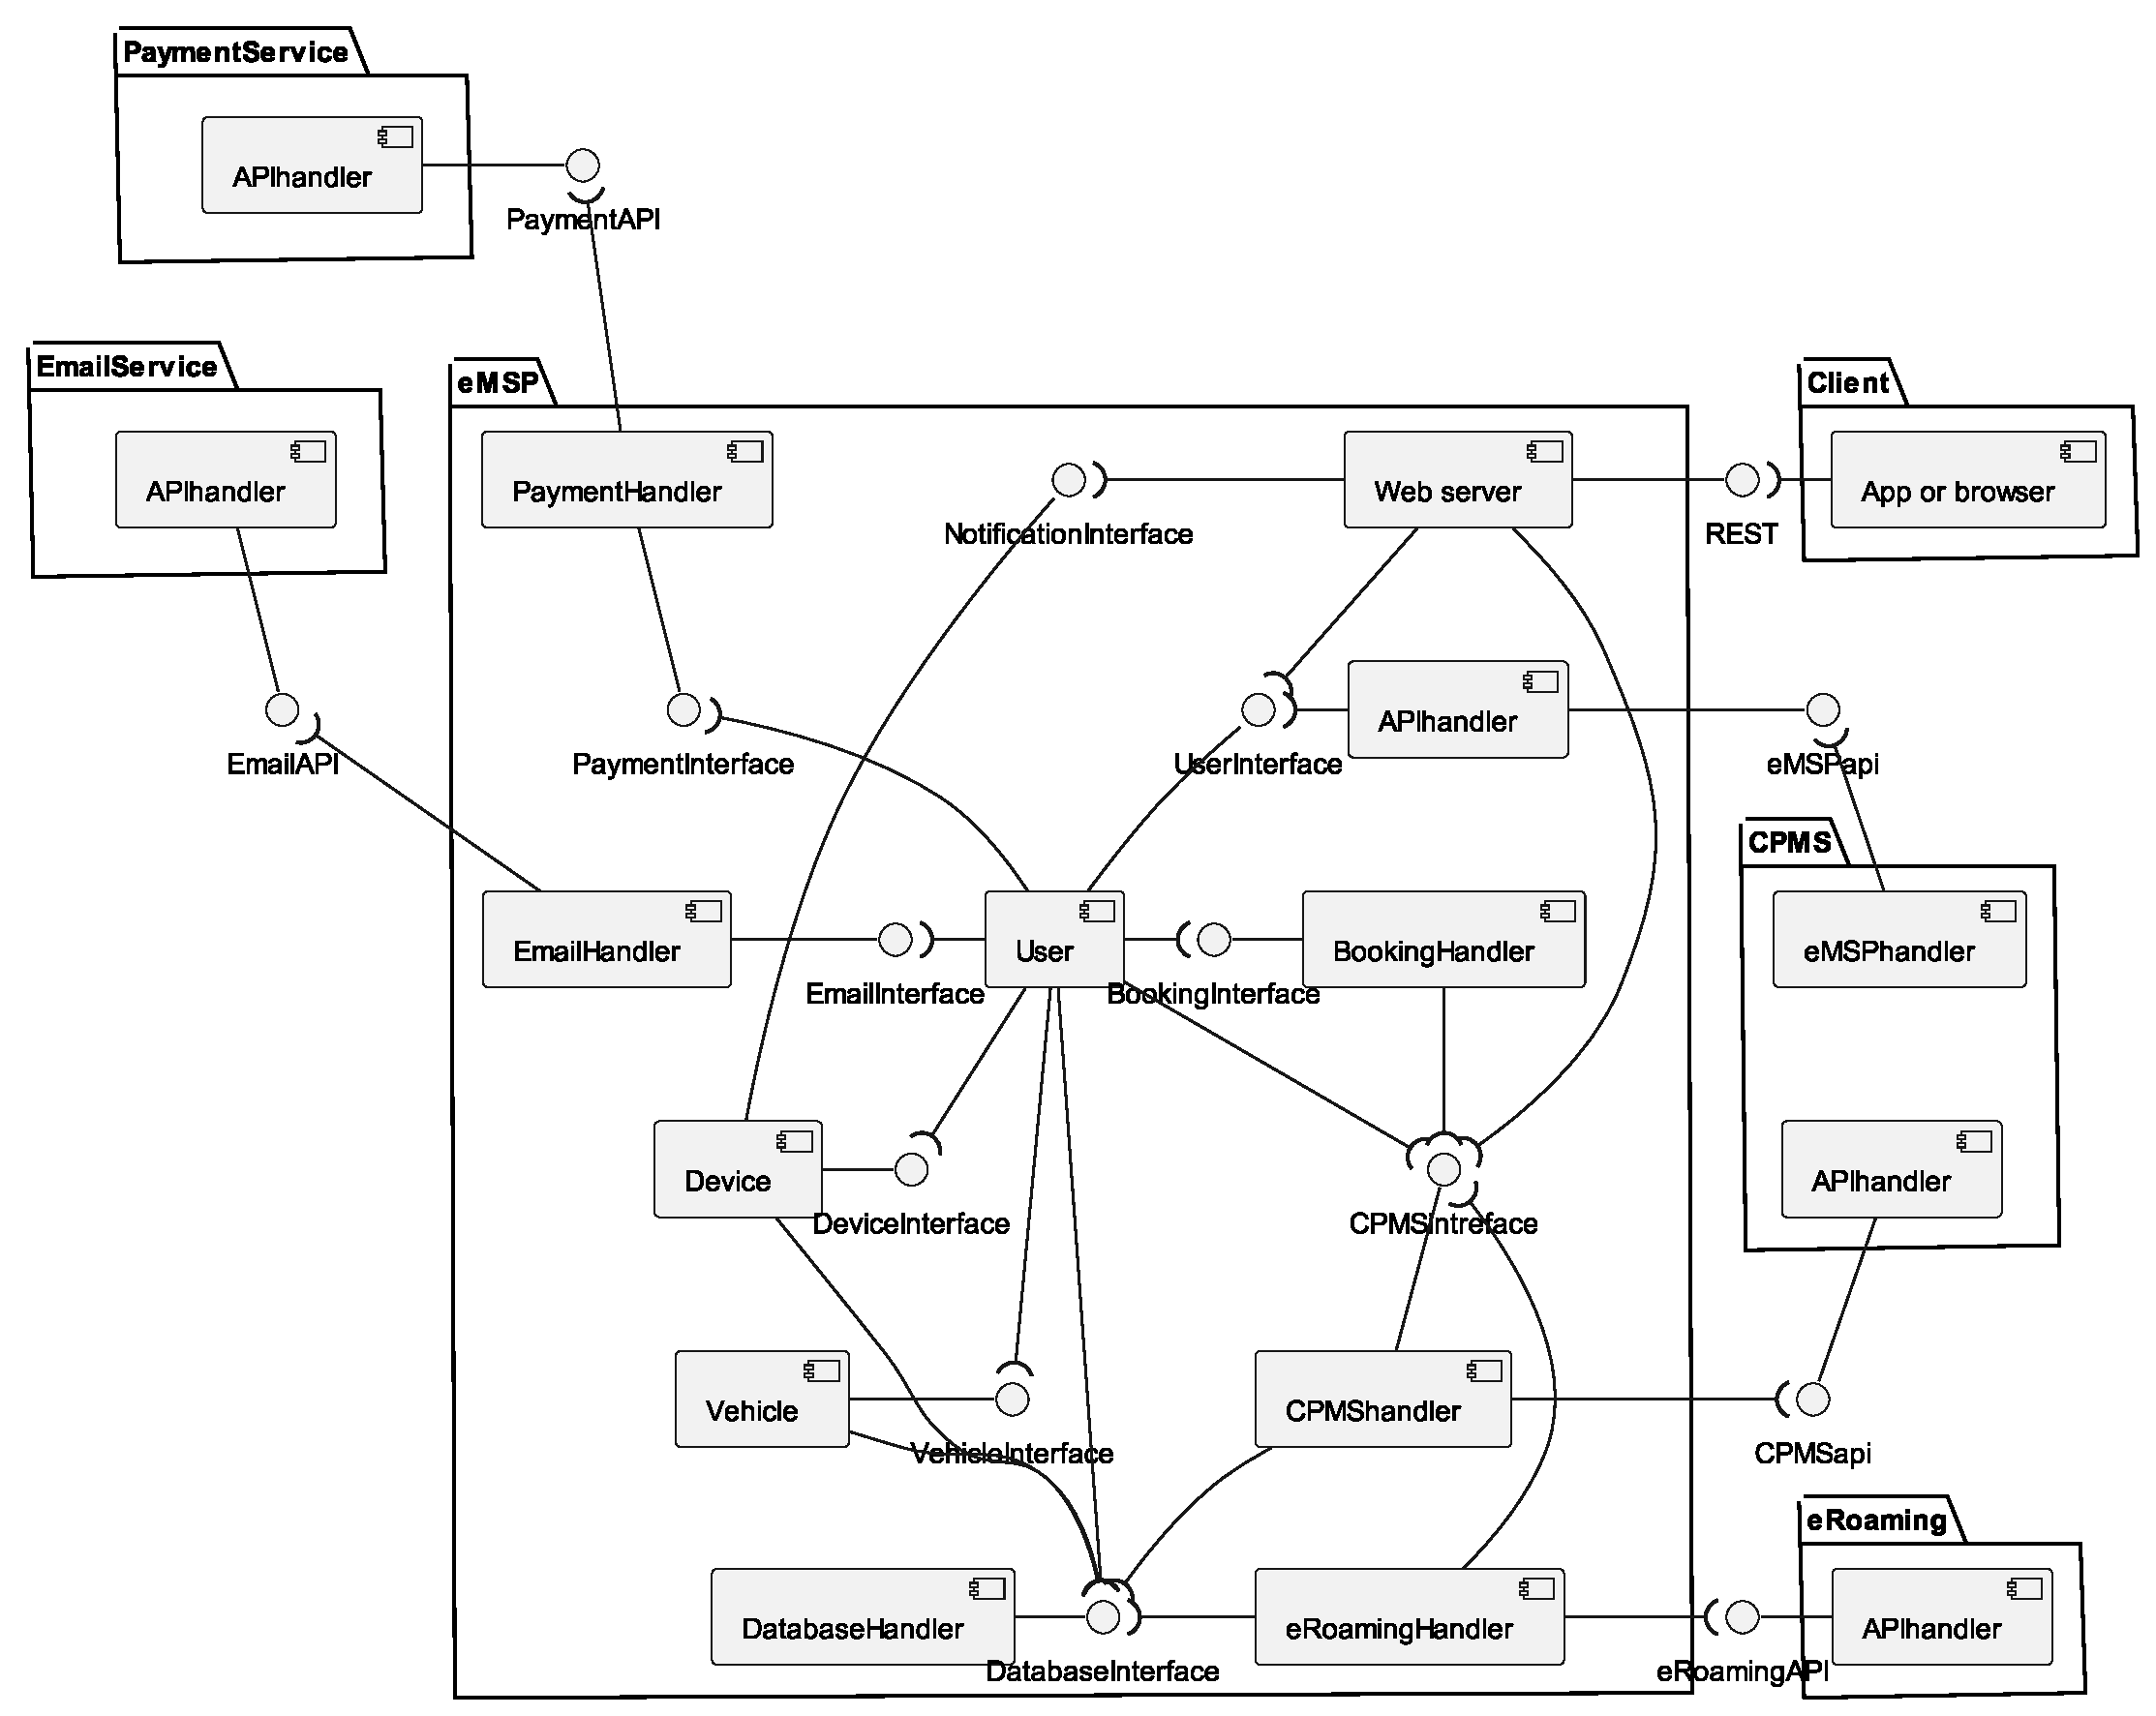
\includegraphics[width=\columnwidth]{./images/components/emsp}
    \caption{connections and interfaces of the eMSP.}
\end{figure}

\paragraph{APIhandler} Manages all the requests coming from any connected CPMS, providing the required data and sending notifications to the user whenever they're needed.

\paragraph{BookingHandler} Manages all the bookings. This is the component that, working together with the \linebreak \texttt{CPMShandler}, allows the user to book a charge, edit and delete it. Please, note that this component is not depicted in the class diagram of the \textit{Requirements Analysis and Specification Document}. This is because here, from an implementation point of view, it's better to separate these functionalities from the \texttt{User} class.

\paragraph{CPMShandler} This is the middleware between the eMPS and the CPMS. It manages all the outgoing requests for the CPMS, like the bookings and any eventual successful payment from the user.

\paragraph{DatabaseHandler} The database contains all the data of the system, and together with its DBMS, it provides all the required data to the above modules. The \texttt{DatabaseInterface} presented here is just a way to represent the various queries that may be done to the database. As a simplification, in the next sections (\reference{view:interfaces} and \reference{view:runtime}) the \texttt{DatabaseInterface} is stated to provide methods for accessing the data. Of course, this is not true in practice since all the queries are written in SQL.

\paragraph{Device} This component manages all the information regarding the users' devices. It is also the one that in case the preferred notification method of the user is the notification one, keeps an open channel with that specific device and sends notifications.

\paragraph{eRoamingHandler} Manages all the processes of connecting with an eRoaming service, inserting all the information about the found CPMSs (directly taken from the found CPOs) in the database.

\paragraph{PaymentHandler} Manages all the financial transactions between the various actors of the system.

\paragraph{User} This is the main component with which the user interacts. It is also the one that provides the devices and vehicle data to the other components.

\paragraph{Vehicle} This component manages all the information regarding the users' vehicles.

\paragraph{Web server} The web server is the frontend of the system for the end user. It statically serves all the page components (it doesn't render anything, it only sends HTML pages, with the required CSS and JavaScript) and replies to the user's HTTP requests through JSON strings.

\subsection{CPMS component view}

\begin{figure}[h!]
    \centering
    \includegraphics[width=\columnwidth]{./images/components/cpms}
    \caption{connections and interfaces of the CPMS.}
\end{figure}

\paragraph {APIhandler} Manages all the requests coming from any connected eMSP, providing the required data and allowing the eMSP users to book charges.

\paragraph {Booking} Handles all the booking of charges, creating and modifying the data stored in the database. It also decides which column to assign to users, communicating the choice by sending a message to the eMSP through the \texttt{eMSPhandler}.

\paragraph {ChargingColumn} Handles the physical charging of the devices. By communicating with the database it's able to establish whether to start or finish the charge based on the bookings present and the certificate of the connected car. Through its interface, it allows observers to be attached. This can be used to send a notification to the owner of the car when the charge ends, as the column itself cannot communicate to the eMSP's API. 

\paragraph {ChargingStation} Handles the choice of DSOs and energy mix in the charging station. If \doublequotes{automatic choice} is selected for either \doublequotes{DSO choice} or \doublequotes{EnergyMix}, it keeps looping querying useful updates, making decisions, and waiting a fixed amount of time, until the mode is deselected. It adds observers to \texttt{EnergySource} and \texttt{ChargingColumn} relative to the station, to have quicker access to important information. In particular, it needs to change the energy mix whenever a station battery reaches 100\% capacity, and it needs to send a message to the car owner whose car's charge ends.

\paragraph {DatabaseHandler} It handles all communication with the database, therefore is used by most components in the CPMS system.

\paragraph {DSOhandler} It handles all communication with the DSO's API. It, therefore, is invoked when the DSO choice changes or when new information from a DSO is queried.

\paragraph {eMSPhandler} It sends messages to the eMSP by communicating with its API.

\paragraph {Energy Source} It represents the various types of sources available in the charging station (batteries, solar panels, and DSO energy). It changes the amount of energy provided by the source. Observers can be attached for various reasons. In batteries, observers can be added to prevent charging over a given threshold or running below a given threshold. 

\paragraph {eRoamingHandler} It handles connections with the eRoaming.

\paragraph {PaymentHandler} It handles connections with the Payment Service, both receiving payments and allowing eMSP users to pay directly at the charging station.

\paragraph {User} It handles all actions that the CPMS user can do through the web interface. It's capable to interact with both \texttt{ChargingStation} and the database to carry out all actions and to query the required information. 

\paragraph {Web Server} It's the frontend of the CPMS website. After login, it holds information like the \texttt{CPMSuserID} and the session token, used in all internal interactions. It communicates with the user via HTTP requests and responses, sending HTML, CSS, and JavaScript files to create the views, then sending JSON strings to send the data.

\pagebreak

\section{Deployment view}

This is the deployment view of the two systems, pointing out the internal architecture of both systems, and the interconnections between themselves and with other external systems (such as the various DSOs and the eRoaming provider).

\begin{figure}[h!]
    \centering
    \includegraphics[width=0.93\columnwidth]{./images/deployment}
    \caption{deployment view of the systems.}
\end{figure}

\paragraph{Client} Depending on the system, the client can connect to it through a desktop/personal computer or through a mobile device (this one is available only for the eMSP consumer since there exists only for it a mobile application and the website is optimized for being viewed from a mobile device). From them, the clients can interact with the system, being able to do all the actions depicted in the \textit{Requirements Analysis and Specification Document}.

\paragraph{Presentation layer} The presentation layer consists of a web server, which acts as a reverse proxy for all the services behind it. In this case, the choice of using NGINX was made because of its event-based nature, and its low memory and CPU footprint. Moreover, it provides a simple configuration for load balancing of the behind components, acting as a reverse proxy (which hides these components from the outside), provides efficient data compression and encryption, which directly provides a higher ranking position in search engines (SEO), and also support live reloads of the configuration in case of updates. NGINX also provides a module for managing JWTs. This is used every time a request is issued from the client in order to verify the authenticity of the incoming requests. If a user doesn't provide a token or the token is invalid, s/he is automatically redirected to the login page.

\paragraph{Business layer} The business layer consist of multiple stateless components which interact with each other through the use of sockets, exchanging JSON messages and querying the underlying database. This choice has been taken to provide better scalability through replication.

\paragraph{Data layer} The data layer consists of a replicated database with Two-Phase Commit which provides a reliable place where to store all the important data of the customers. This data source is shared between all the components of the above business layer, but it's accessed directly by a single type of component which translates all the requests to SQL and the results back in suitable JSONs.

\paragraph{Firewalls} Firewalls are an essential part of the whole design. They provide a way to limit the attack surface of any potential intruder by providing strict access rules. Moreover, there are firewalls between the frontend (presentation layer) and the business layer, and between this last one and the data layer. In order to further enhance security, all those depicted firewalls can be extended with some traffic analyzers which actively or passively react to any potential intrusion.

\pagebreak

\section{Components interfaces} \label{view:interfaces}

Here are presented the internal interfaces of each subsystem (the arrows denote a \doublequotes{use} relationship). They are used in the sequence diagrams of the following section \reference{view:runtime}, but some of their calls may be presented in the other system's diagrams. As an example, the eMSP's function \linebreak \texttt{manageNotification (user, message)} taken from the \texttt{UserInterface} maps the call of the CPMS's \linebreak \texttt{sendNotification (eMSPuserID, message)} presented in the sequence diagrams.

\paragraph{Attention} These diagrams (and also the ones in section \reference{view:runtime}) present the interfaces of the components like functions, but, since they communicate through suitable JSONs, they aren't actual functions. It's just a way of modeling more compactly the types of messages and arguments all the various JSONs are built on.

\subsection{eMSP}

This picture depicts the internal interfaces of the eMSP system together with their functions. These allow the user to interact with the system, like booking a charge, and the CPMS to communicate with him/her, like indirectly sending notifications.\medskip

Note that all the components don't directly interact with the underlying database, but they query the \texttt{DatabaseHandler} through its \texttt{DatabaseInterface}, which is the only one to directly access the database.

\begin{figure}[h!]
    \centering
    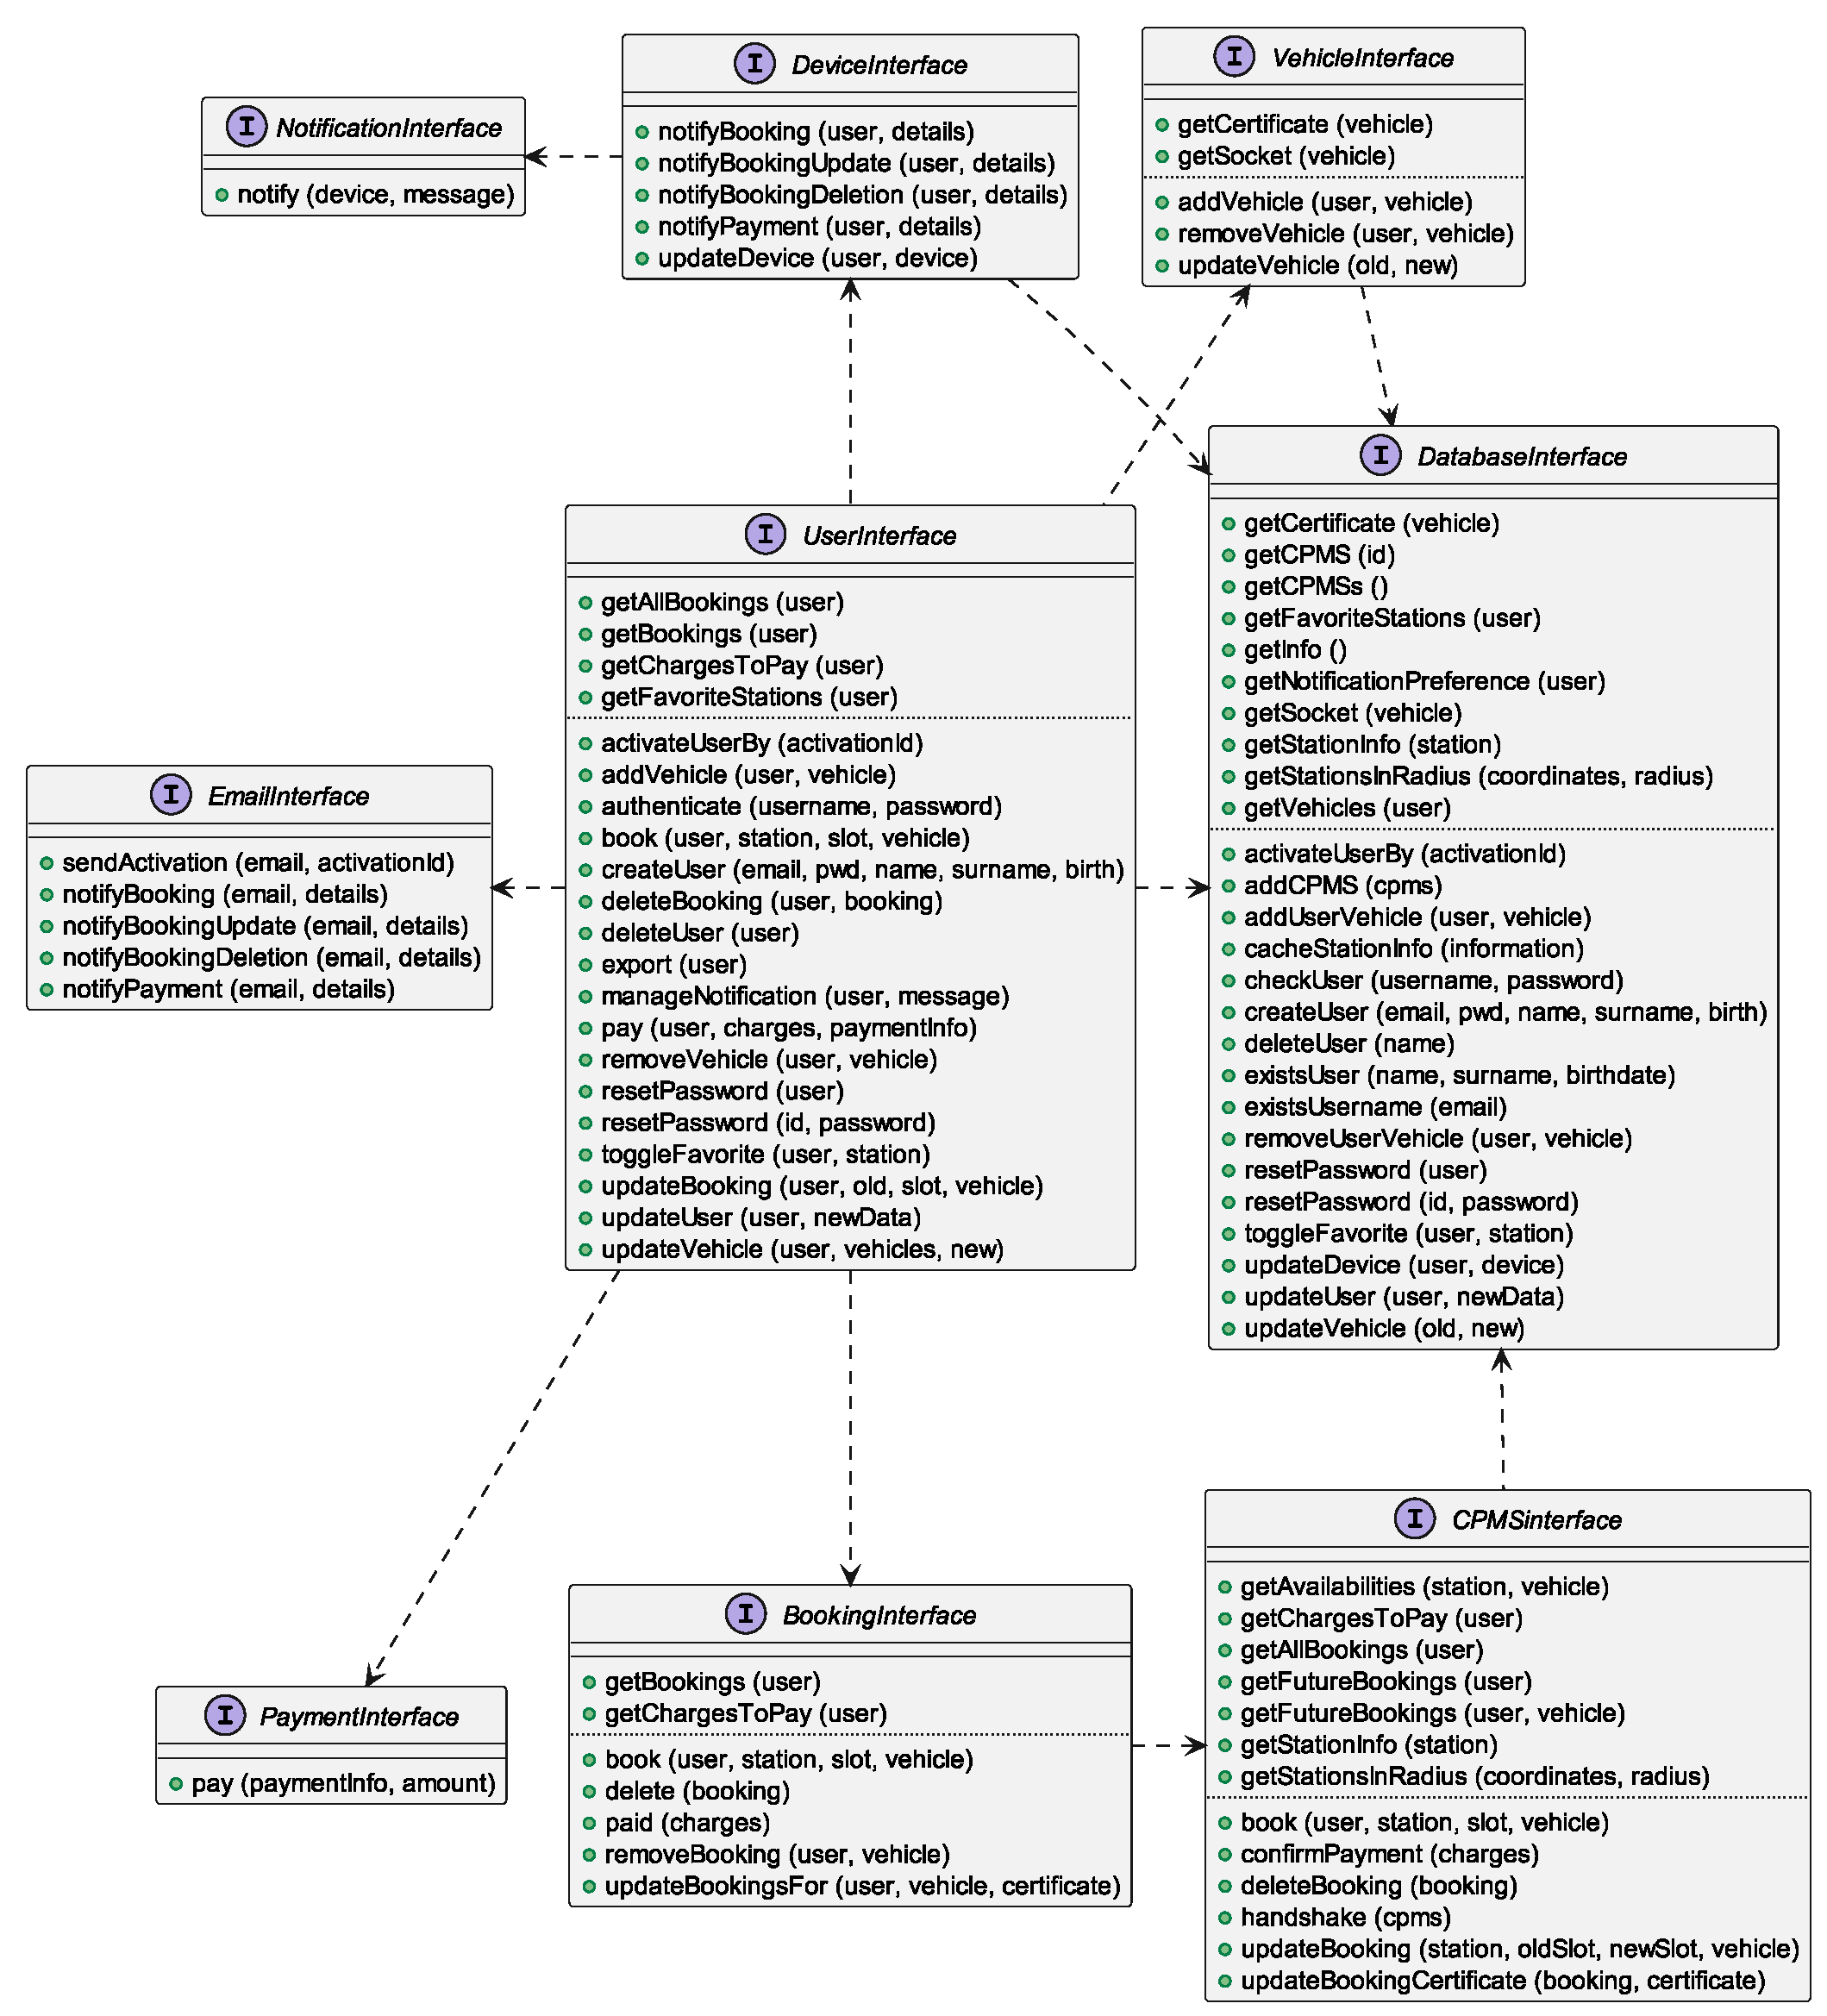
\includegraphics[width=0.84\columnwidth]{./images/interfaces/emsp}
    \caption{internal interfaces of the eMSP system and their functions.}
\end{figure}

\subsection{CPMS}

\figureref{figure:interface:cpms} depicts the internal interfaces of the CPMS system. The functions inside the interfaces cover all functionalities implemented by the CPMS system and/or needed by the eMSP system, and can be improved for future versions of these systems.\medskip

Most interfaces in the CPMS systems make use of the \texttt{DatabaseInterface}, to write to durable storage all changes happening to the system. This is done to be able to recover quickly in case of failures, in order to guarantee the promised availability. Most functions offered in components' interfaces make use of the same function or a similar function offered by the \texttt{DatabaseInterface}, since the \texttt{DatabaseHandler} is the only component that directly communicates with the database.

\begin{figure}[h!]
    \centering
    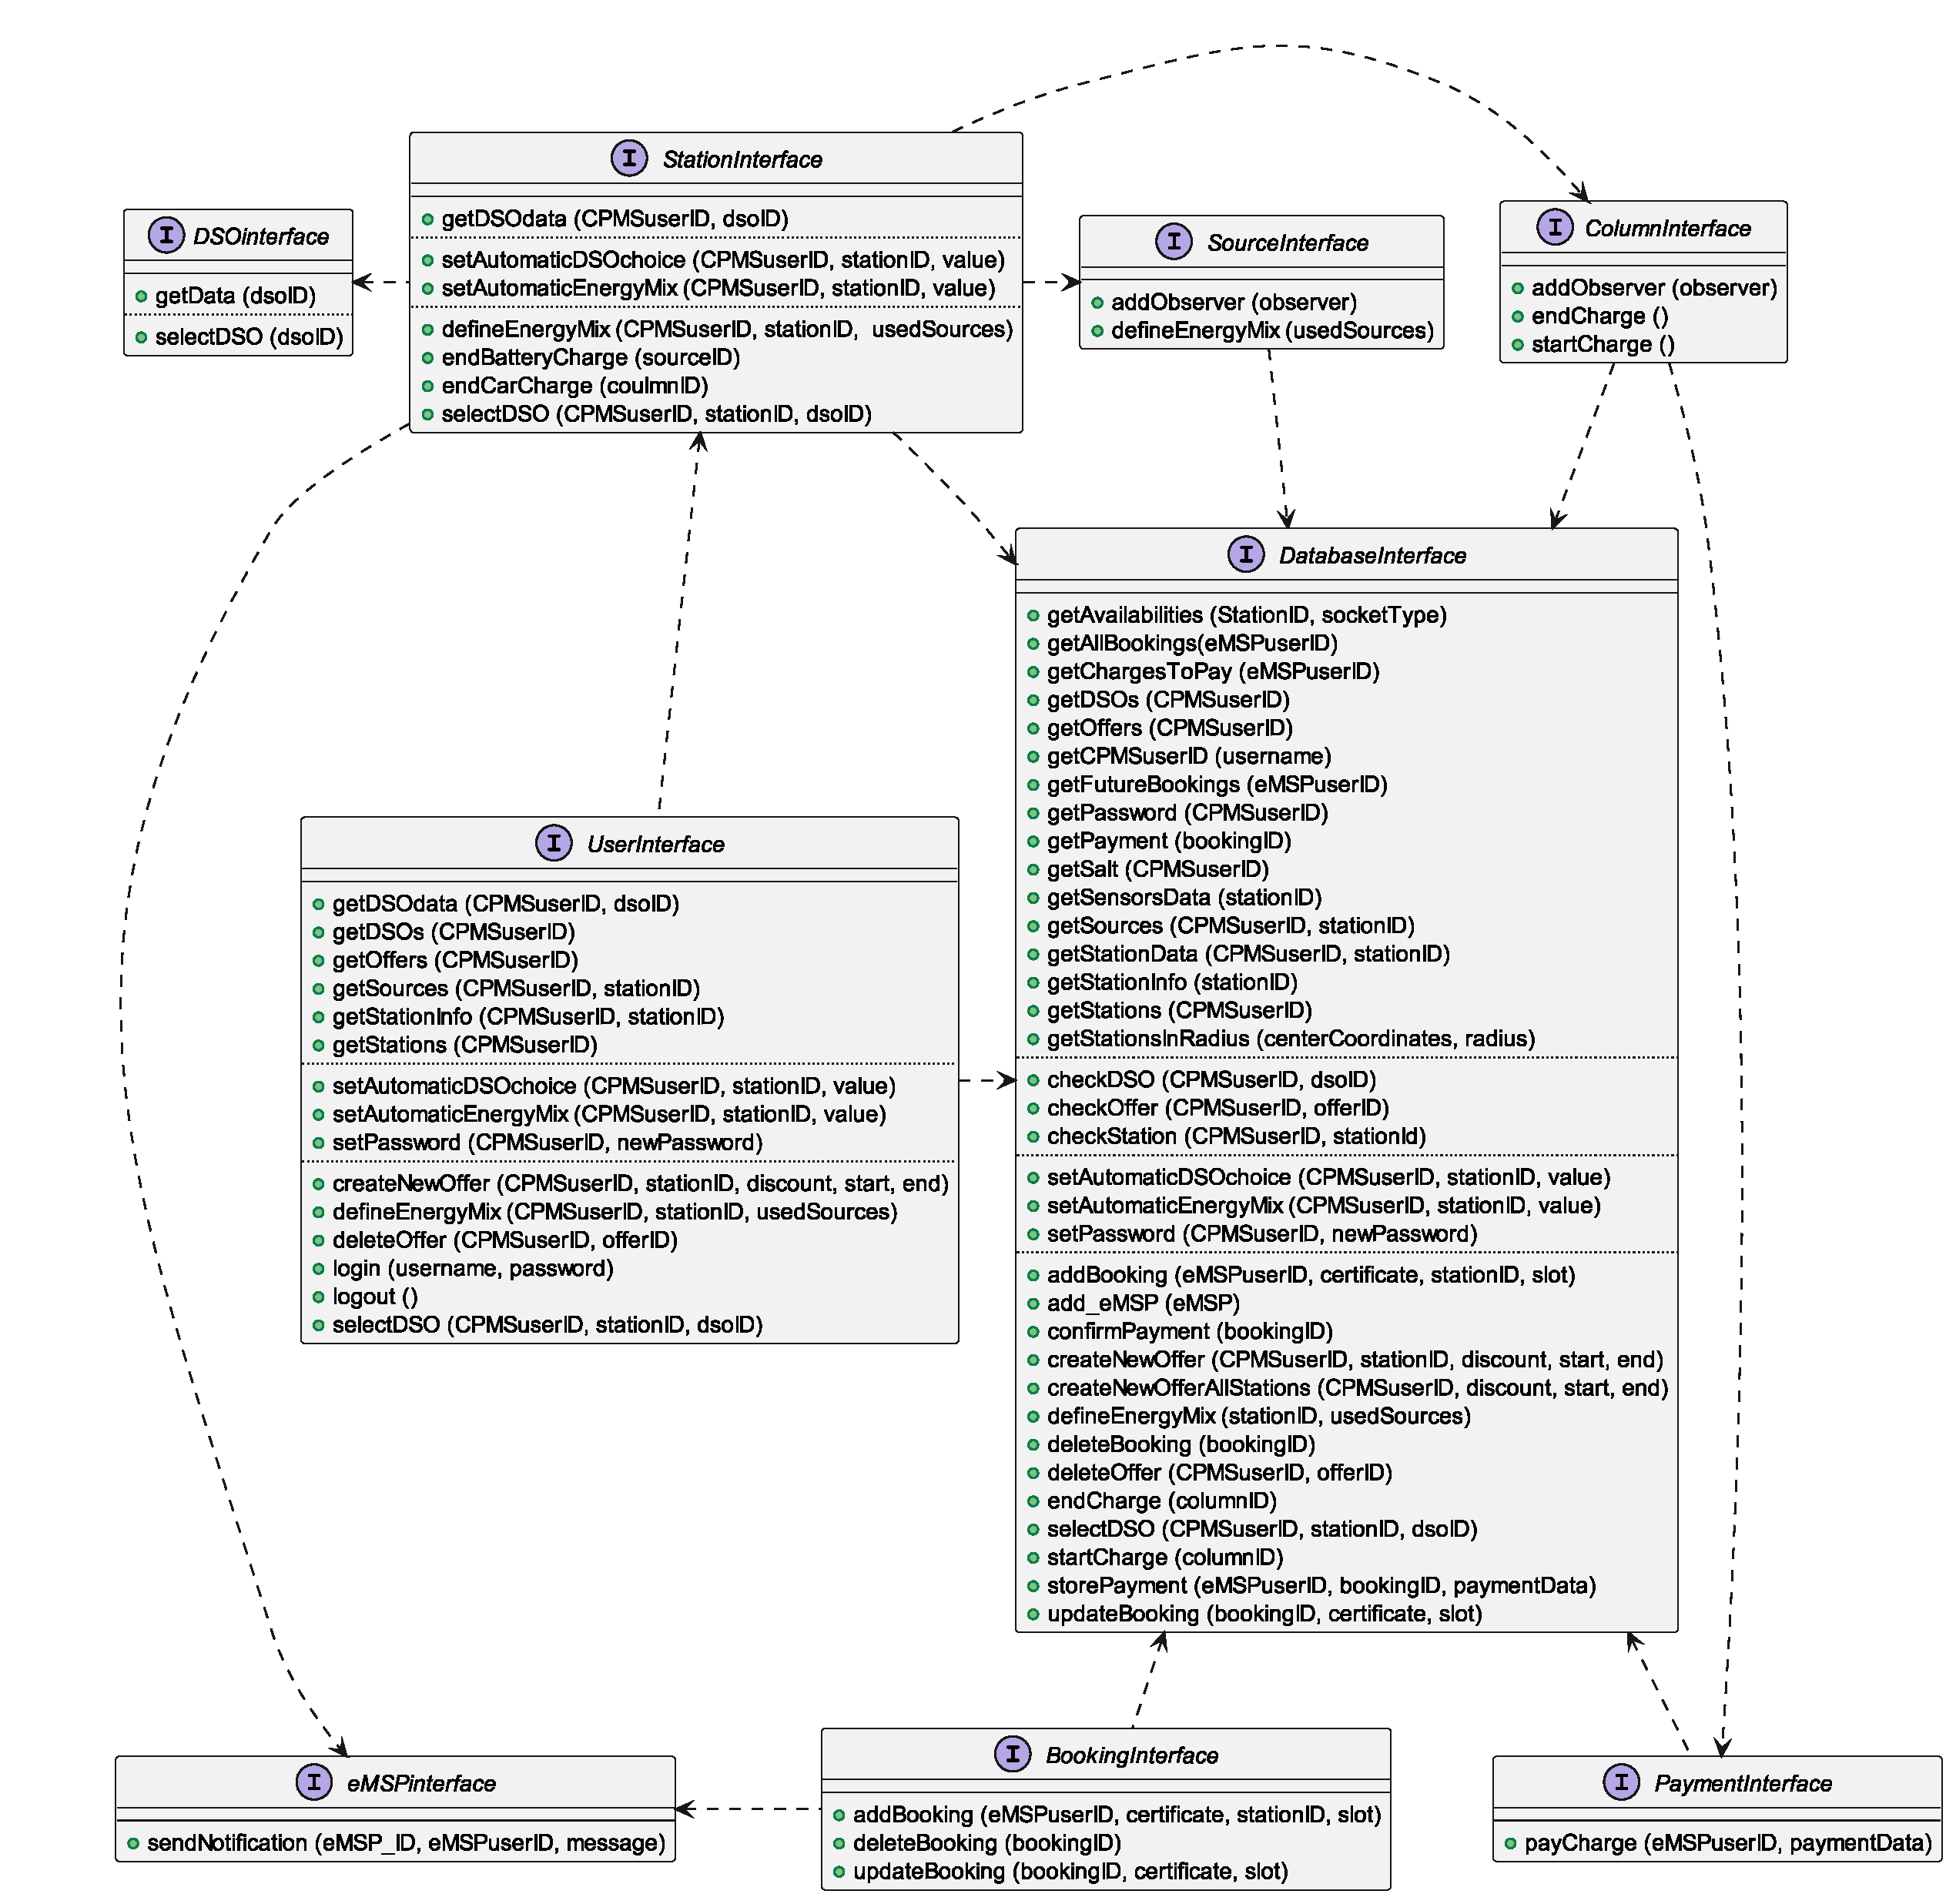
\includegraphics[width=\columnwidth]{./images/interfaces/cpms}
    \caption{internal interfaces of the CPMS system and their functions.}
    \label{figure:interface:cpms}
\end{figure}

\pagebreak

\section{Runtime view} \label{view:runtime}

Here are presented some important actions the user or the system does and how the various components are activated through which function calls in order to perform the required actions.\medskip

Every time \doublequotes{consumer} or \doublequotes{user} appears in a UML diagram, it's intended that s/he is interacting with the application or web page that interacts with the system.\medskip

For the sake of simplicity, many data checks and the opening of the application or web page, according to the use case, are not illustrated, but they are present in the system. Moreover, some cases are not depicted here:
\begin{itemize}
    \item \textit{Notification preference}: the user is asked to choose between in-app notifications or email ones after his first login. Furthermore, the user can change this preference at any time under his/her profile.
    \item \textit{Logout}: simply removes the token from the client.
    \item \textit{Password change}: it works like most of the password changes implemented nowadays. The first option is that the user clicks on the \doublequotes{Forgot password?} link, receives an email with the link for changing it, and changes the password. The second one is that s/he goes to the user's details page and changes the password directly from there. In both cases, s/he has to log back in on all his/her connected devices.
\end{itemize}
Also, even if it's not specified in the diagrams, if any component fails, the user is notified and the action is automatically aborted, reverting its state to the original one. The same happens in case of user's network failures (which are \doublequotes{detected} through a timeout).

\subsection{eMSP}

\paragraph{Registration} The user registers into the system providing the required data through a dedicated form and his/her email address which is then used for sending the activation link and eventual notifications.

\begin{figure}[h!]
    \centering
    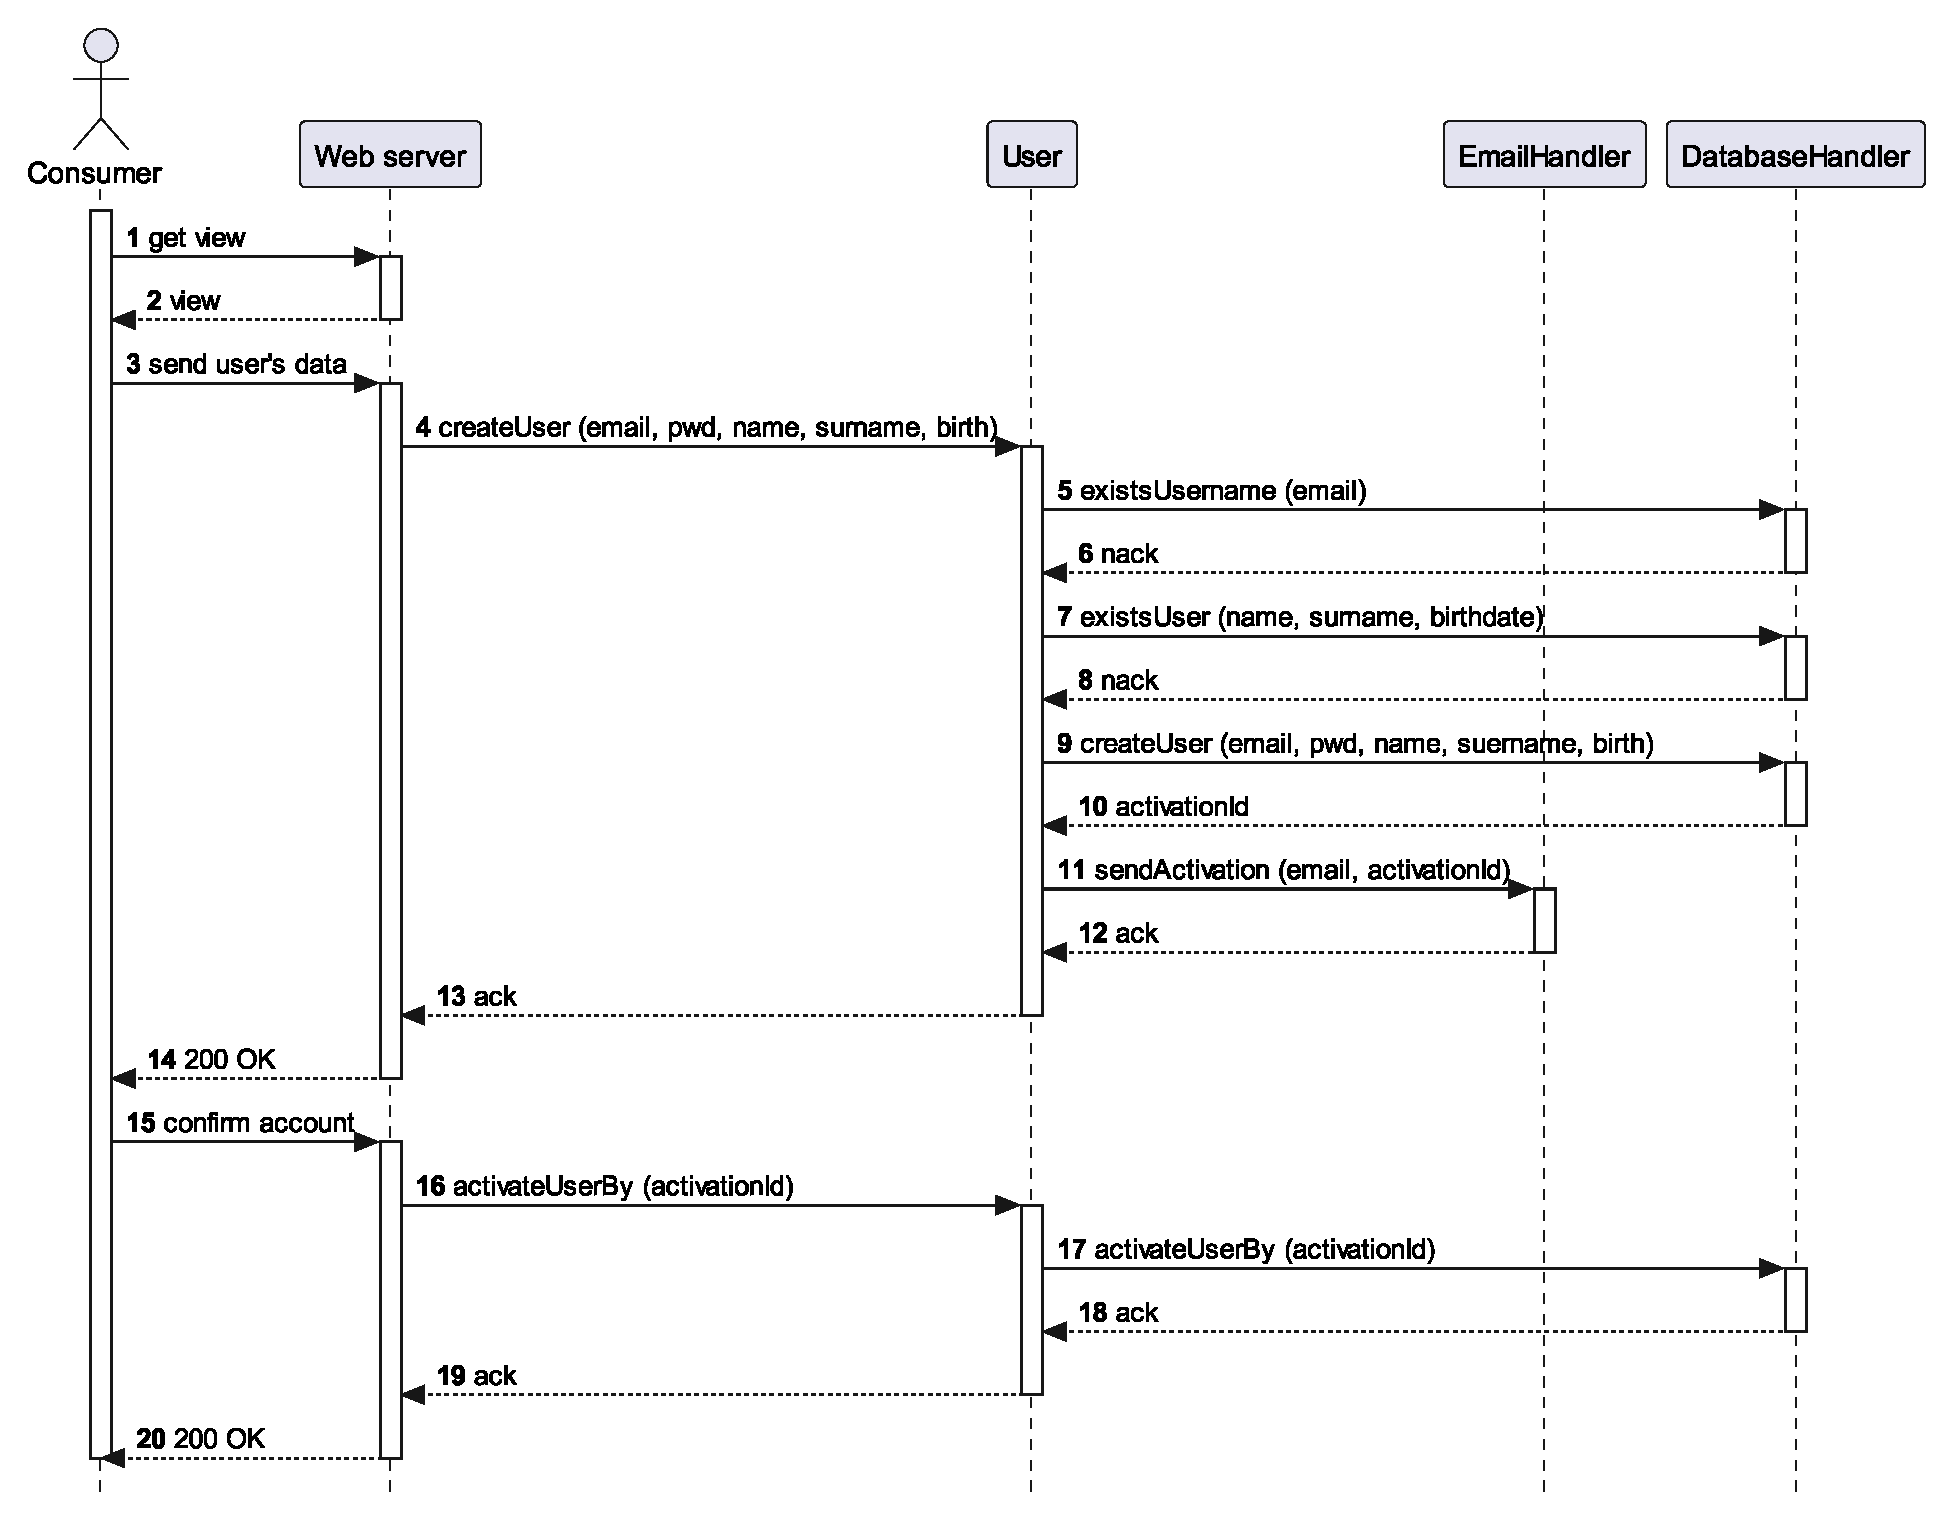
\includegraphics[width=\columnwidth]{./images/sequences/emsp/registration}
    \caption{registration of the eMSP user (consumer).}
\end{figure}

\pagebreak

\paragraph{Login} The user logs into the system, which recognizes him/her and sends back a signed JWT for future actions on the system, like booking charges. This token is properly checked on every request by the web server.

\begin{figure}[h!]
    \centering
    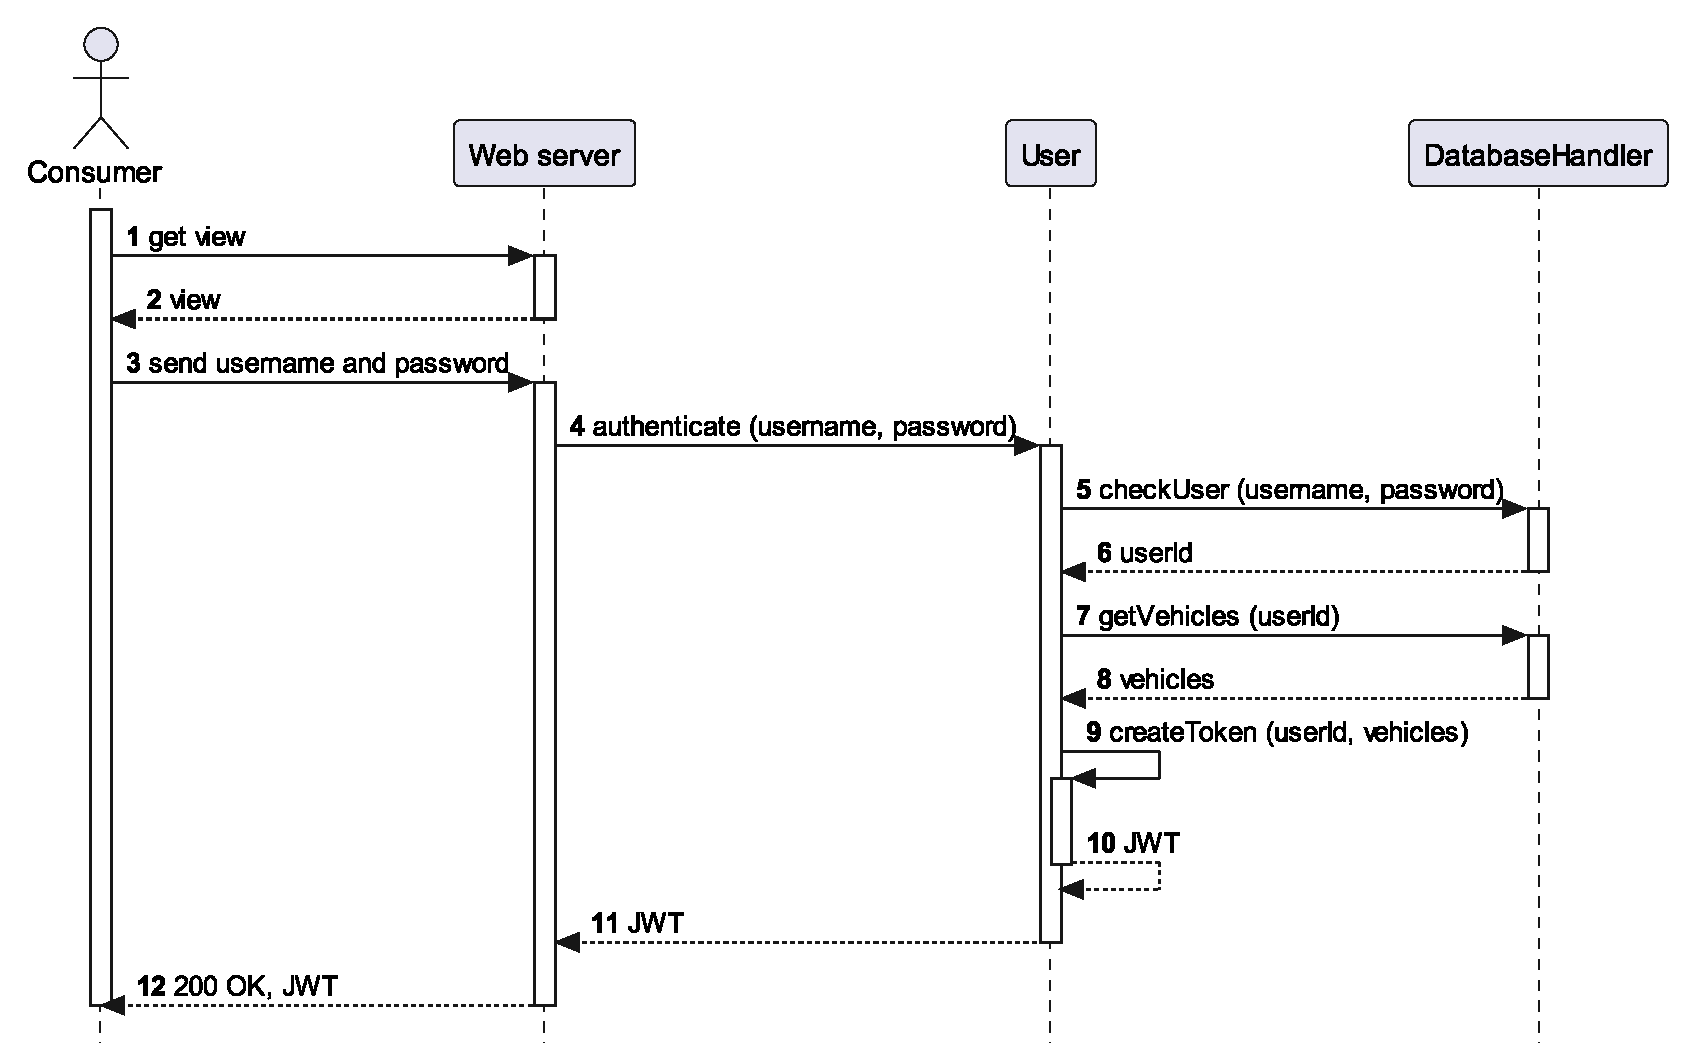
\includegraphics[width=\columnwidth]{./images/sequences/emsp/login}
    \caption{login of the eMSP user (consumer).}
\end{figure}

\paragraph{Mark/unmark a station as favorite} The user marks or unmarks any wanted charging station as favorite. The following diagram shows how the stations can be found thanks to this system.

\begin{figure}[h!]
    \centering
    
\includegraphics[width=0.9\columnwidth]{./images/sequences/emsp/favorite}
    \caption{the user marks/unmarks a station as \doublequotes{favorite}.}
\end{figure}

\pagebreak

\paragraph{Look for nearby stations} The user looks for a charging station, either by searching a location or by using a geolocalization service. In any case it's possible to use the map or the list view.

\begin{figure}[h!]
    \centering
    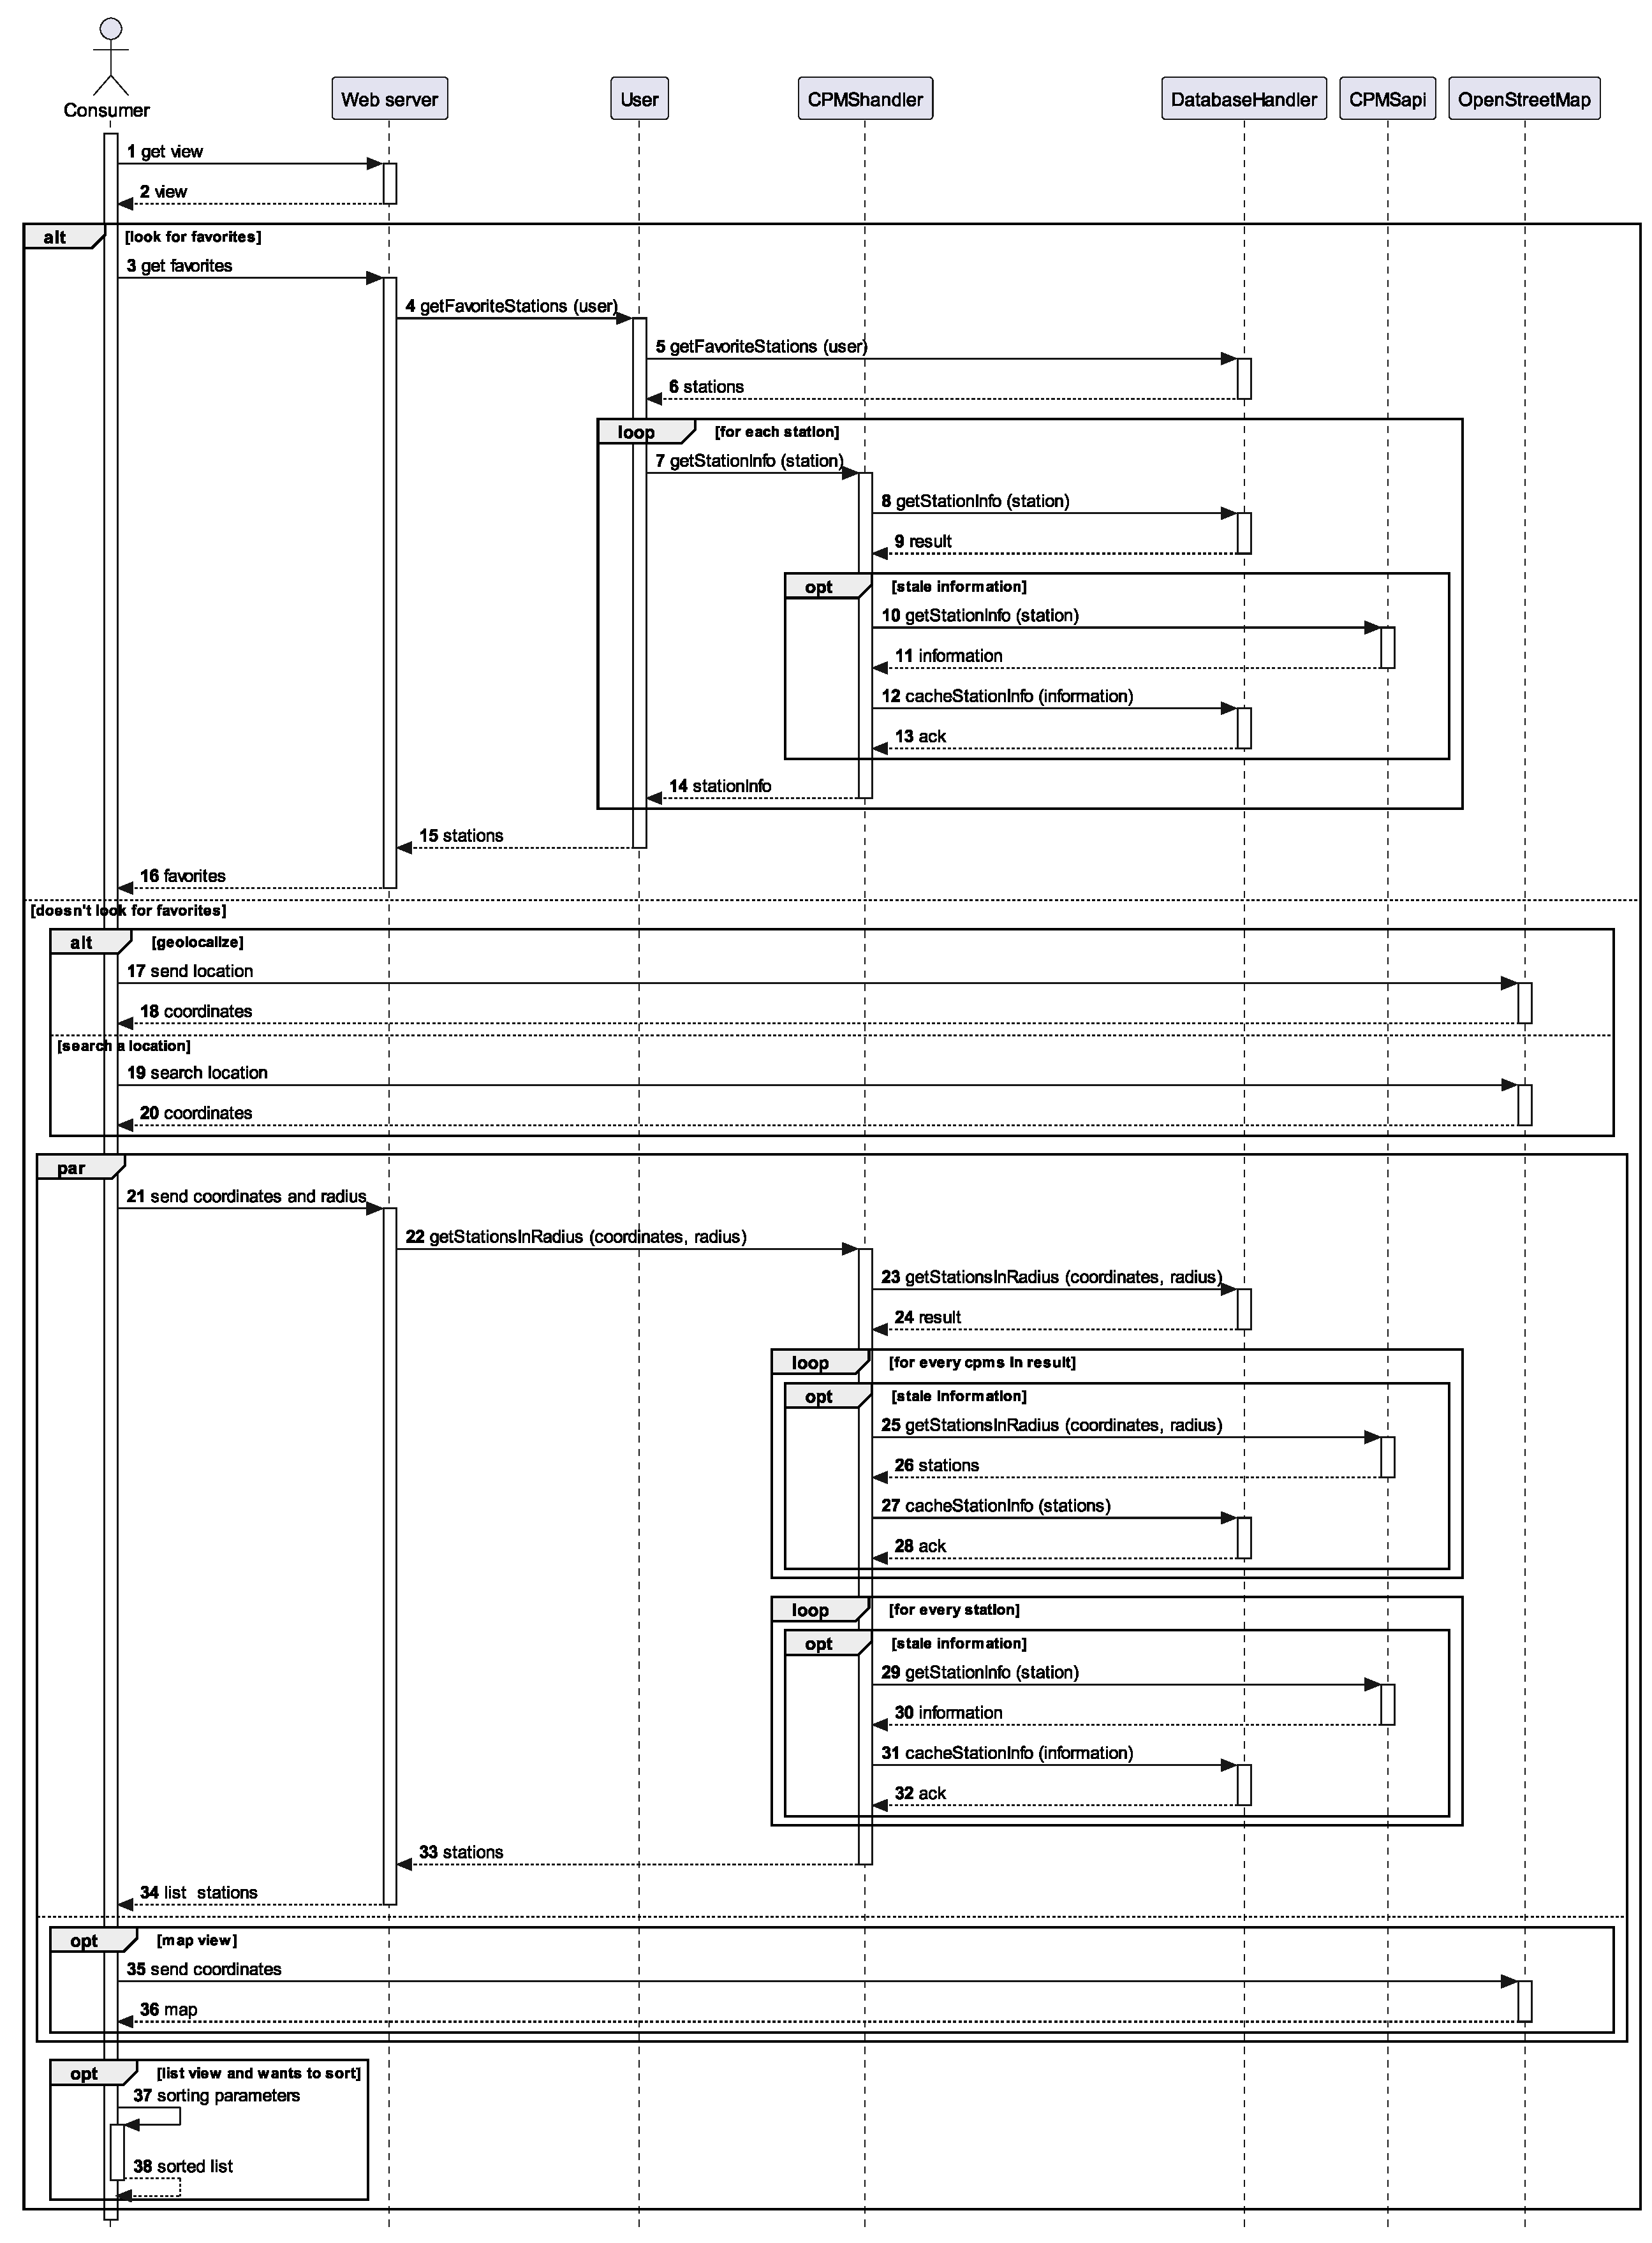
\includegraphics[width=\columnwidth]{./images/sequences/emsp/lookup}
    \caption{the user looks for a charging station.}
\end{figure}

\pagebreak

\paragraph{Book a charge} After finding a suitable station (which is depicted in the previous diagram), the user can book a charge by providing the required data to the system.

\begin{figure}[h!]
    \centering
    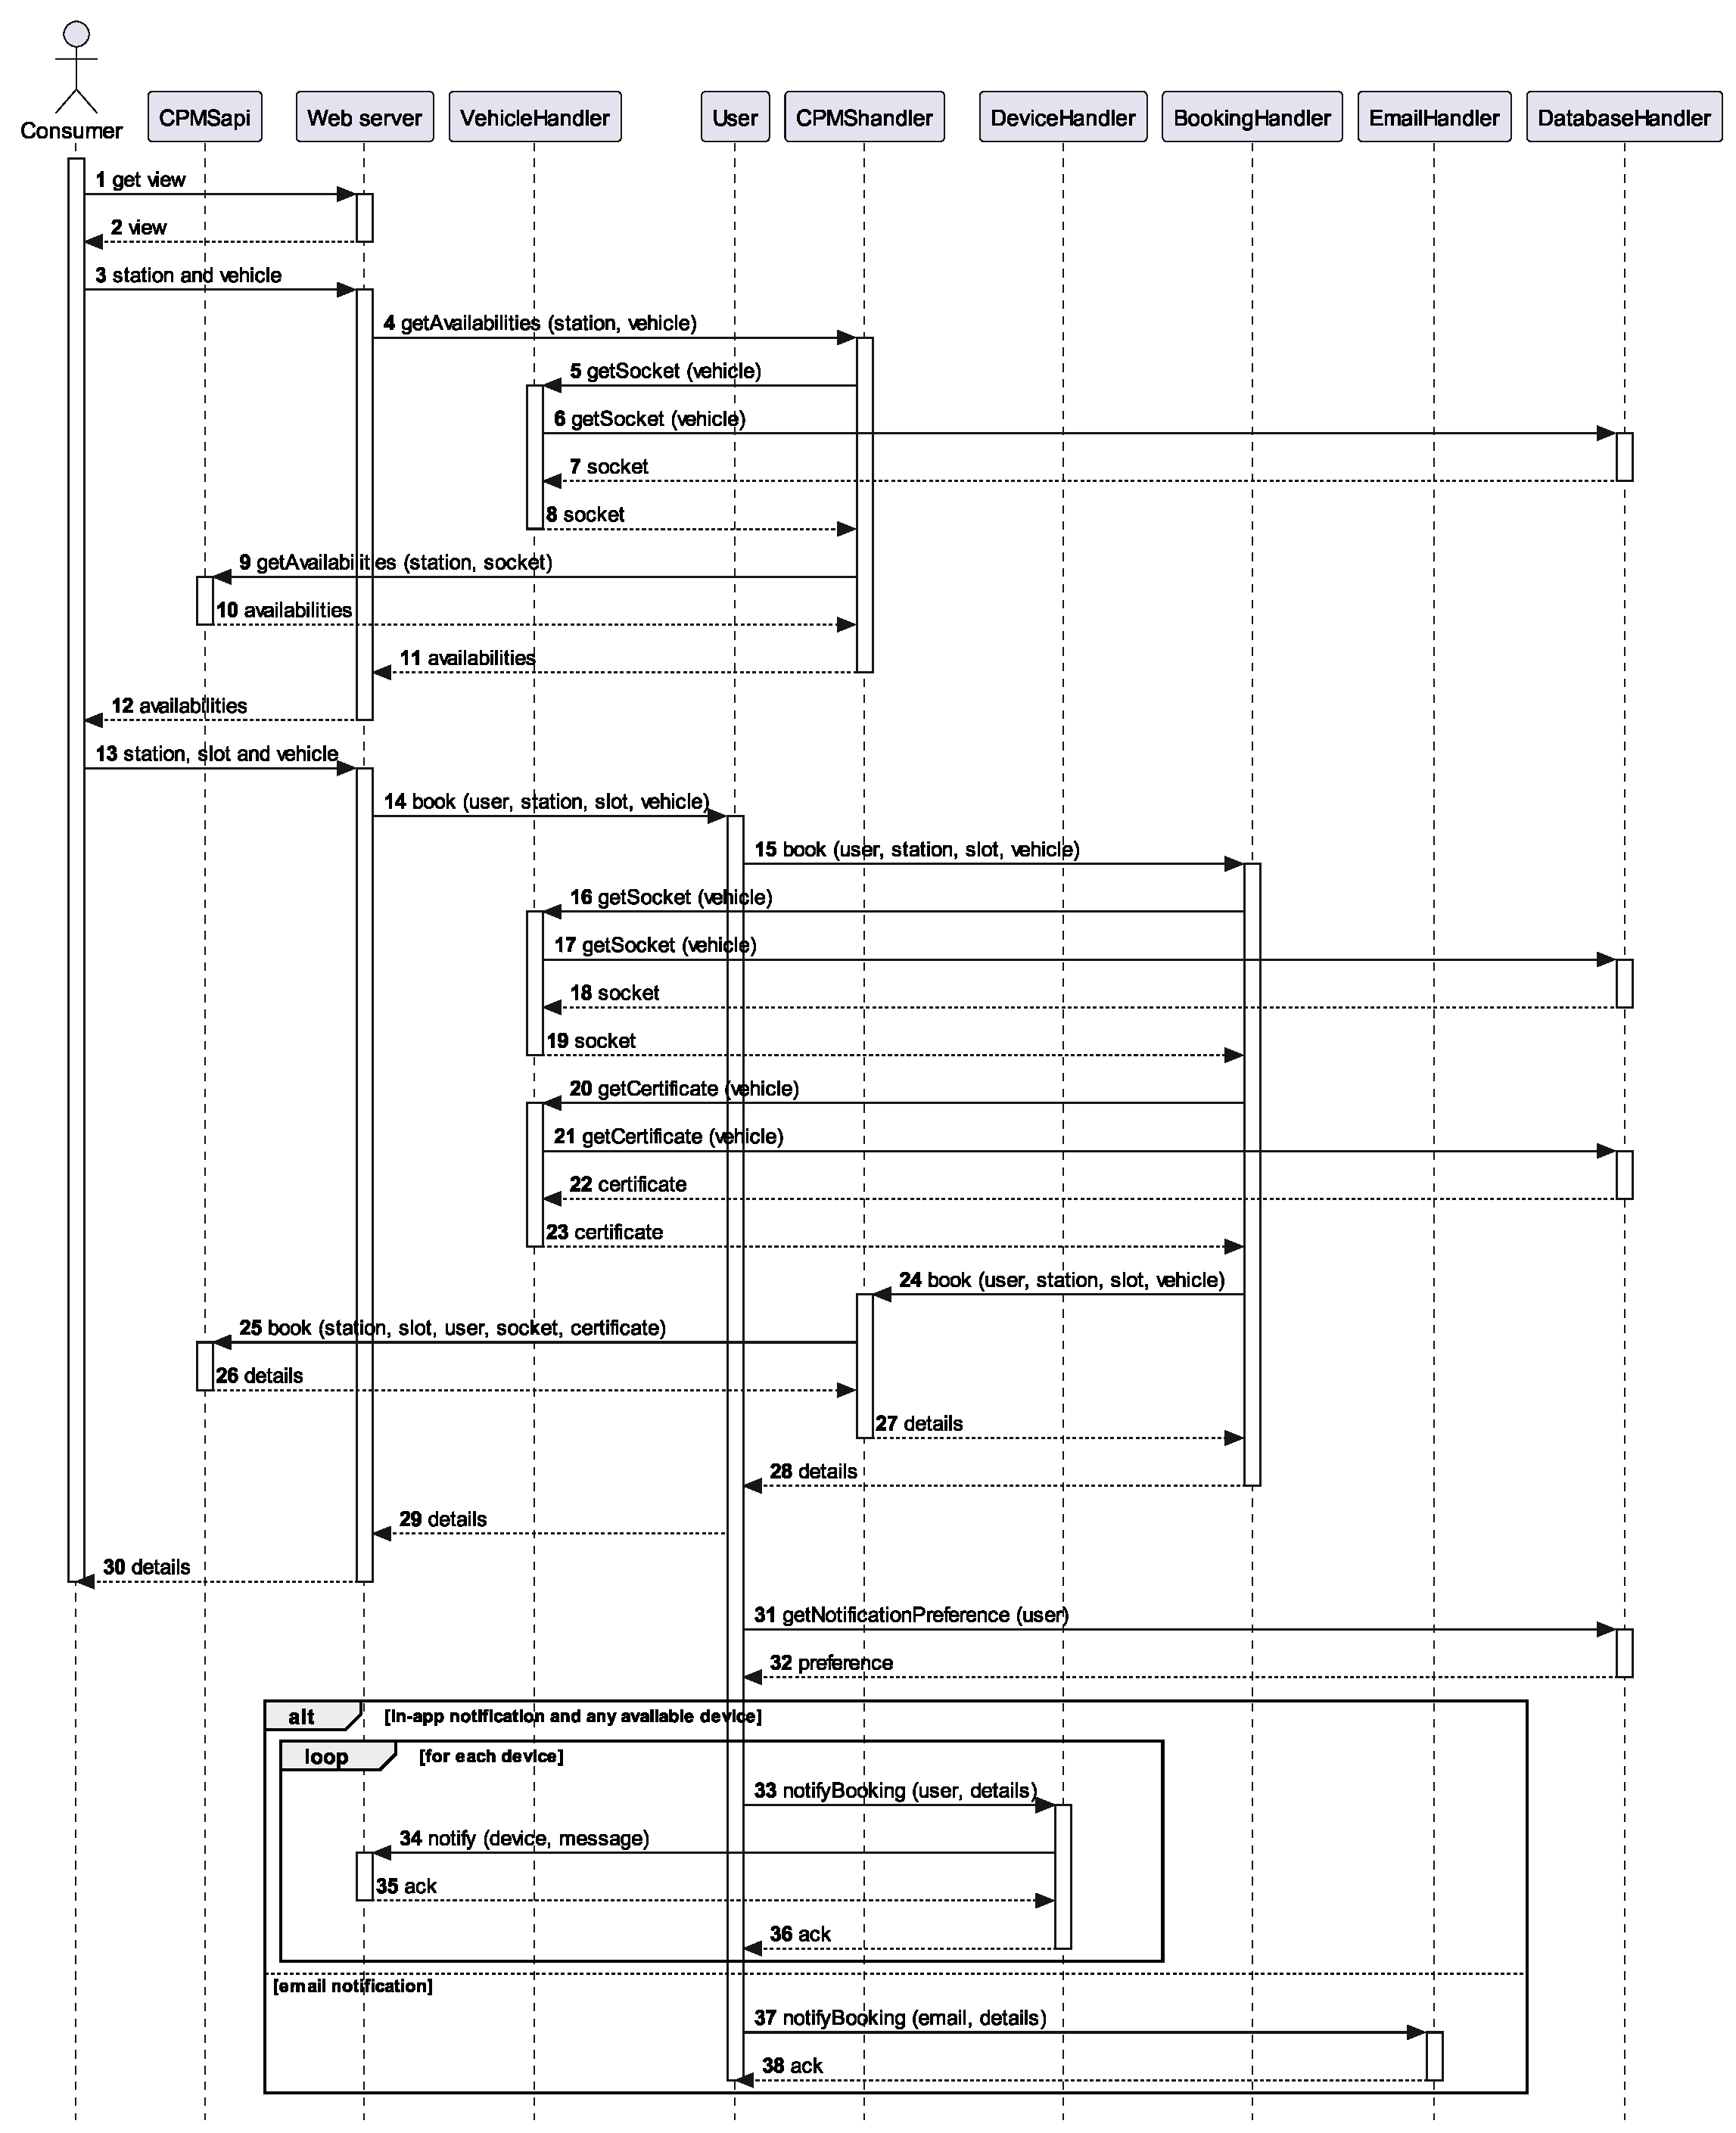
\includegraphics[width=\columnwidth]{./images/sequences/emsp/book_add}
    \caption{the user books a charge.}
\end{figure}

\pagebreak

\paragraph{Edit a reservation} If the user needs to, it's possible to modify an already existing booked charge for the same station, providing the required data.

\begin{figure}[h!]
    \centering
    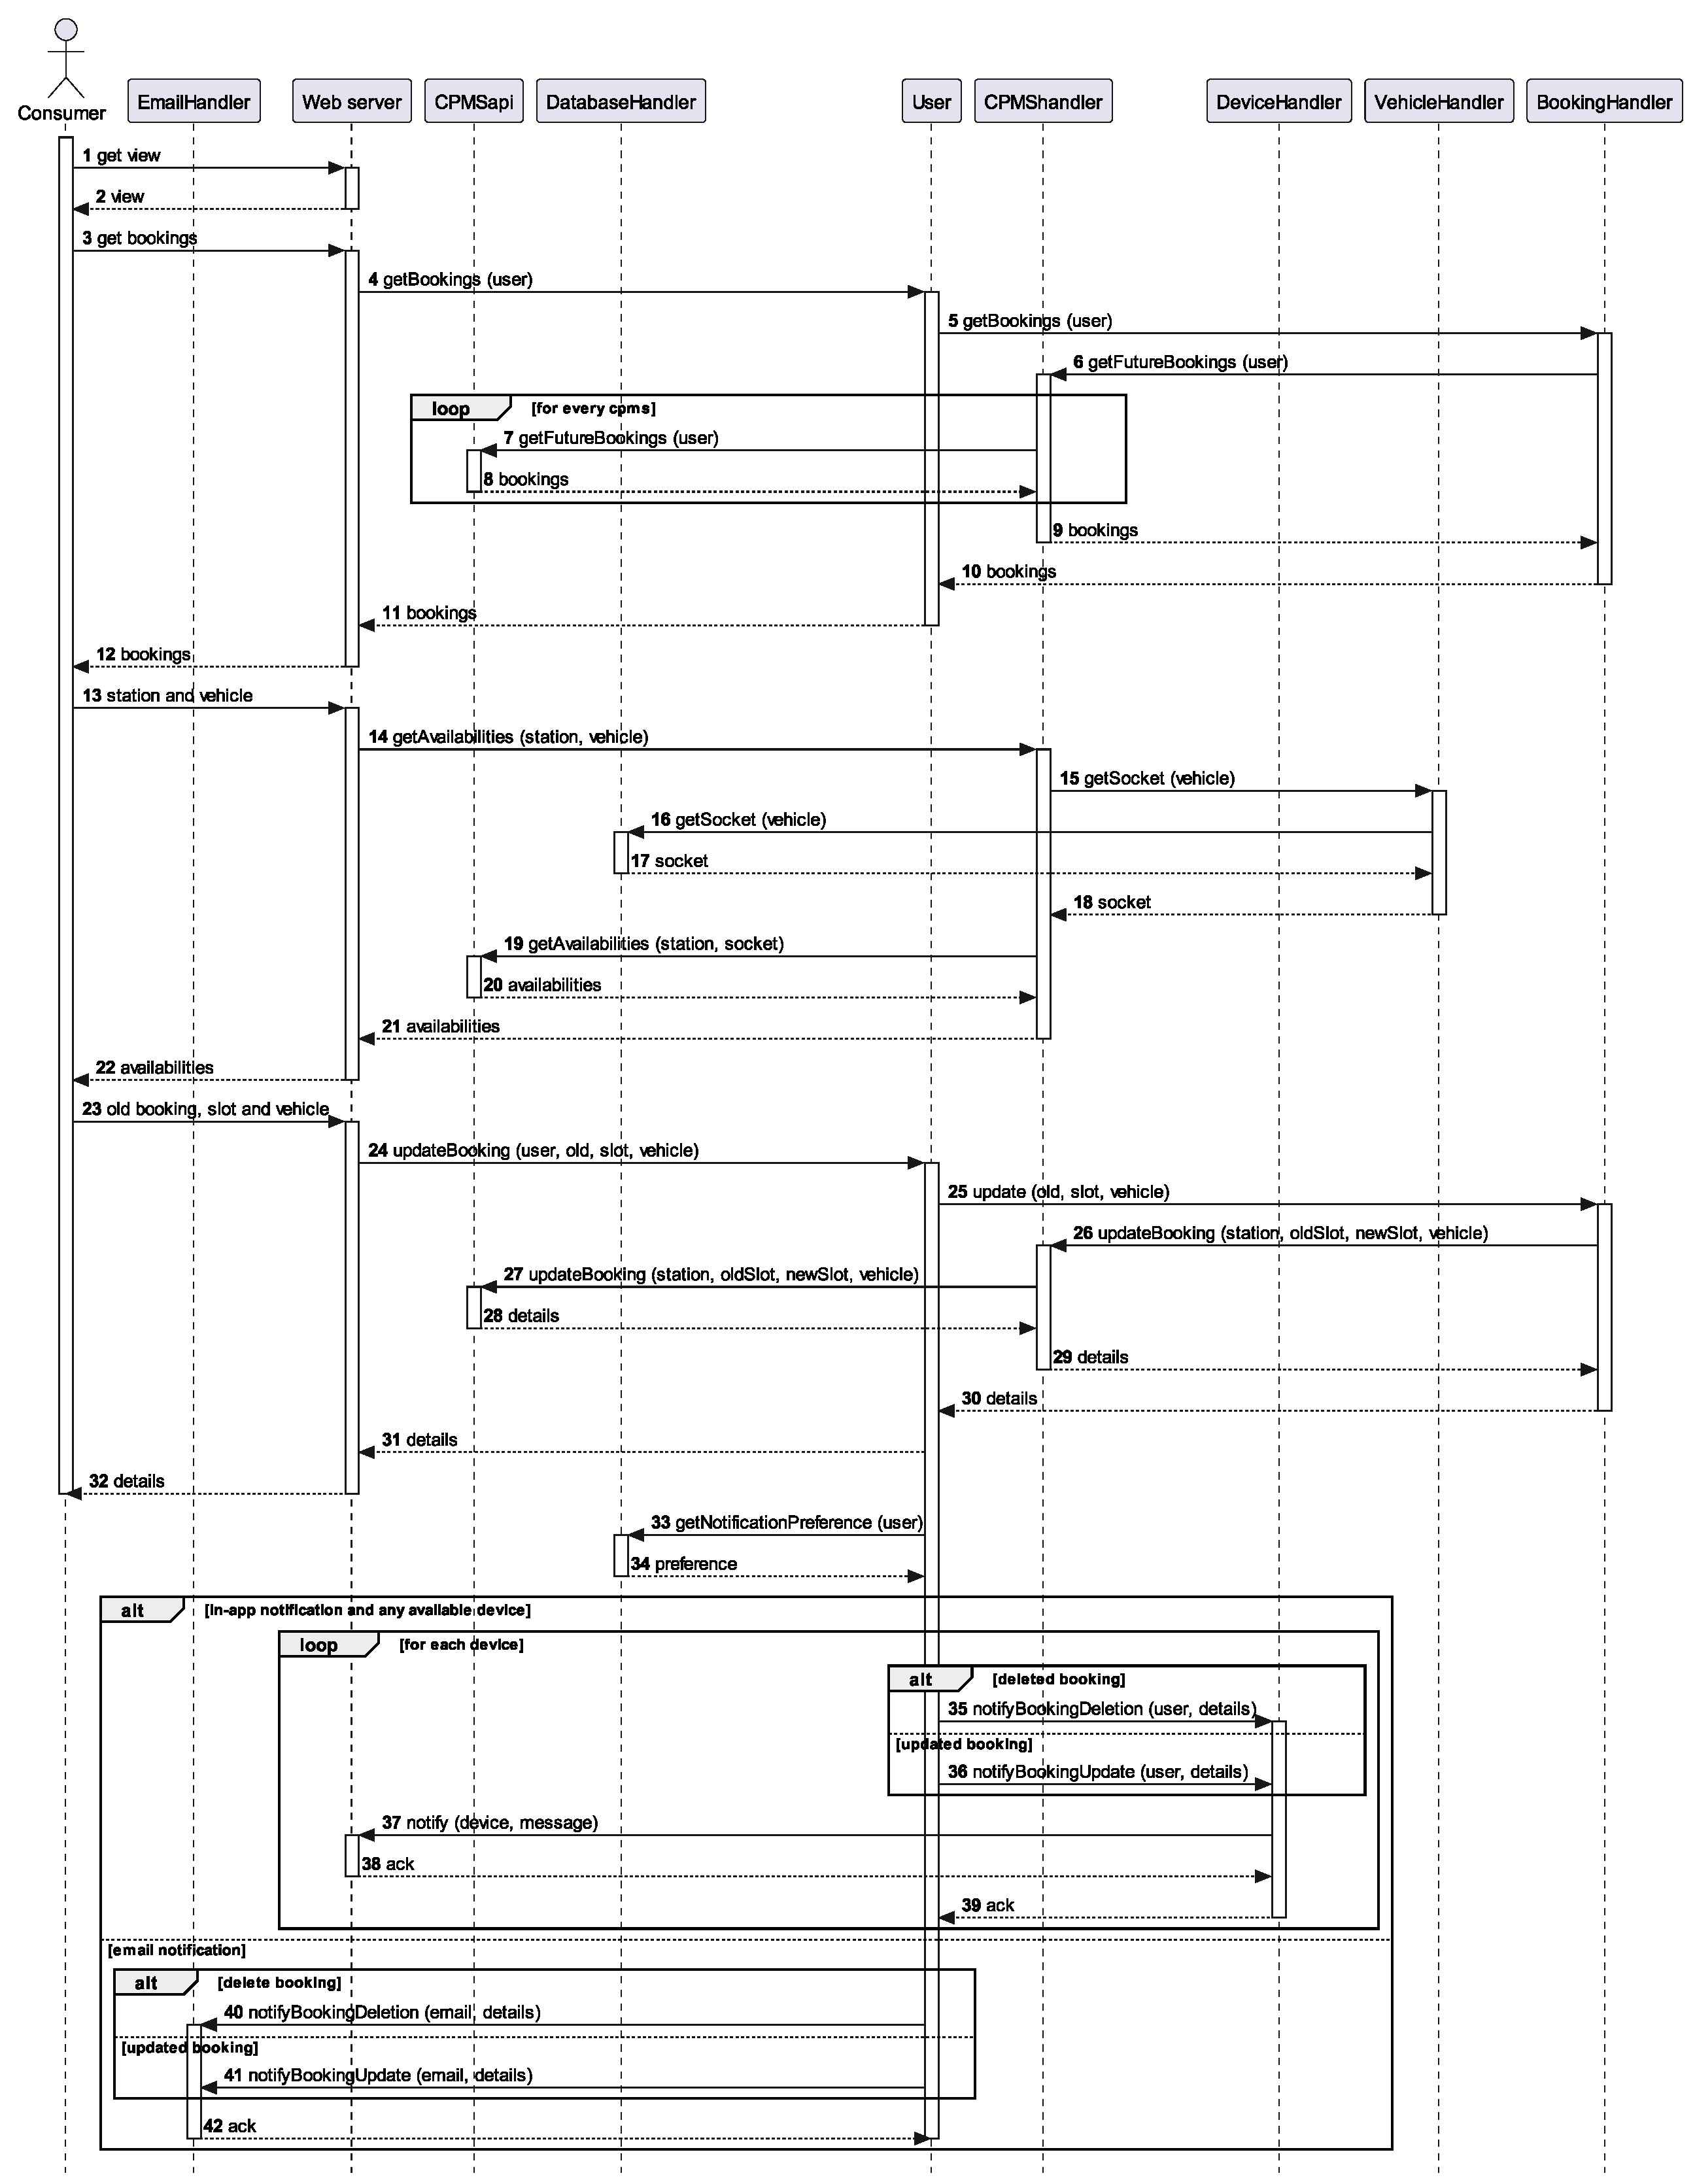
\includegraphics[width=\columnwidth]{./images/sequences/emsp/book_edit}
    \caption{the user edits a booked charge.}
\end{figure}

\pagebreak

\paragraph{Delete a reservation} If the user needs to, it's possible to delete a previously booked charge unless it's in the past.

\begin{figure}[h!]
    \centering
    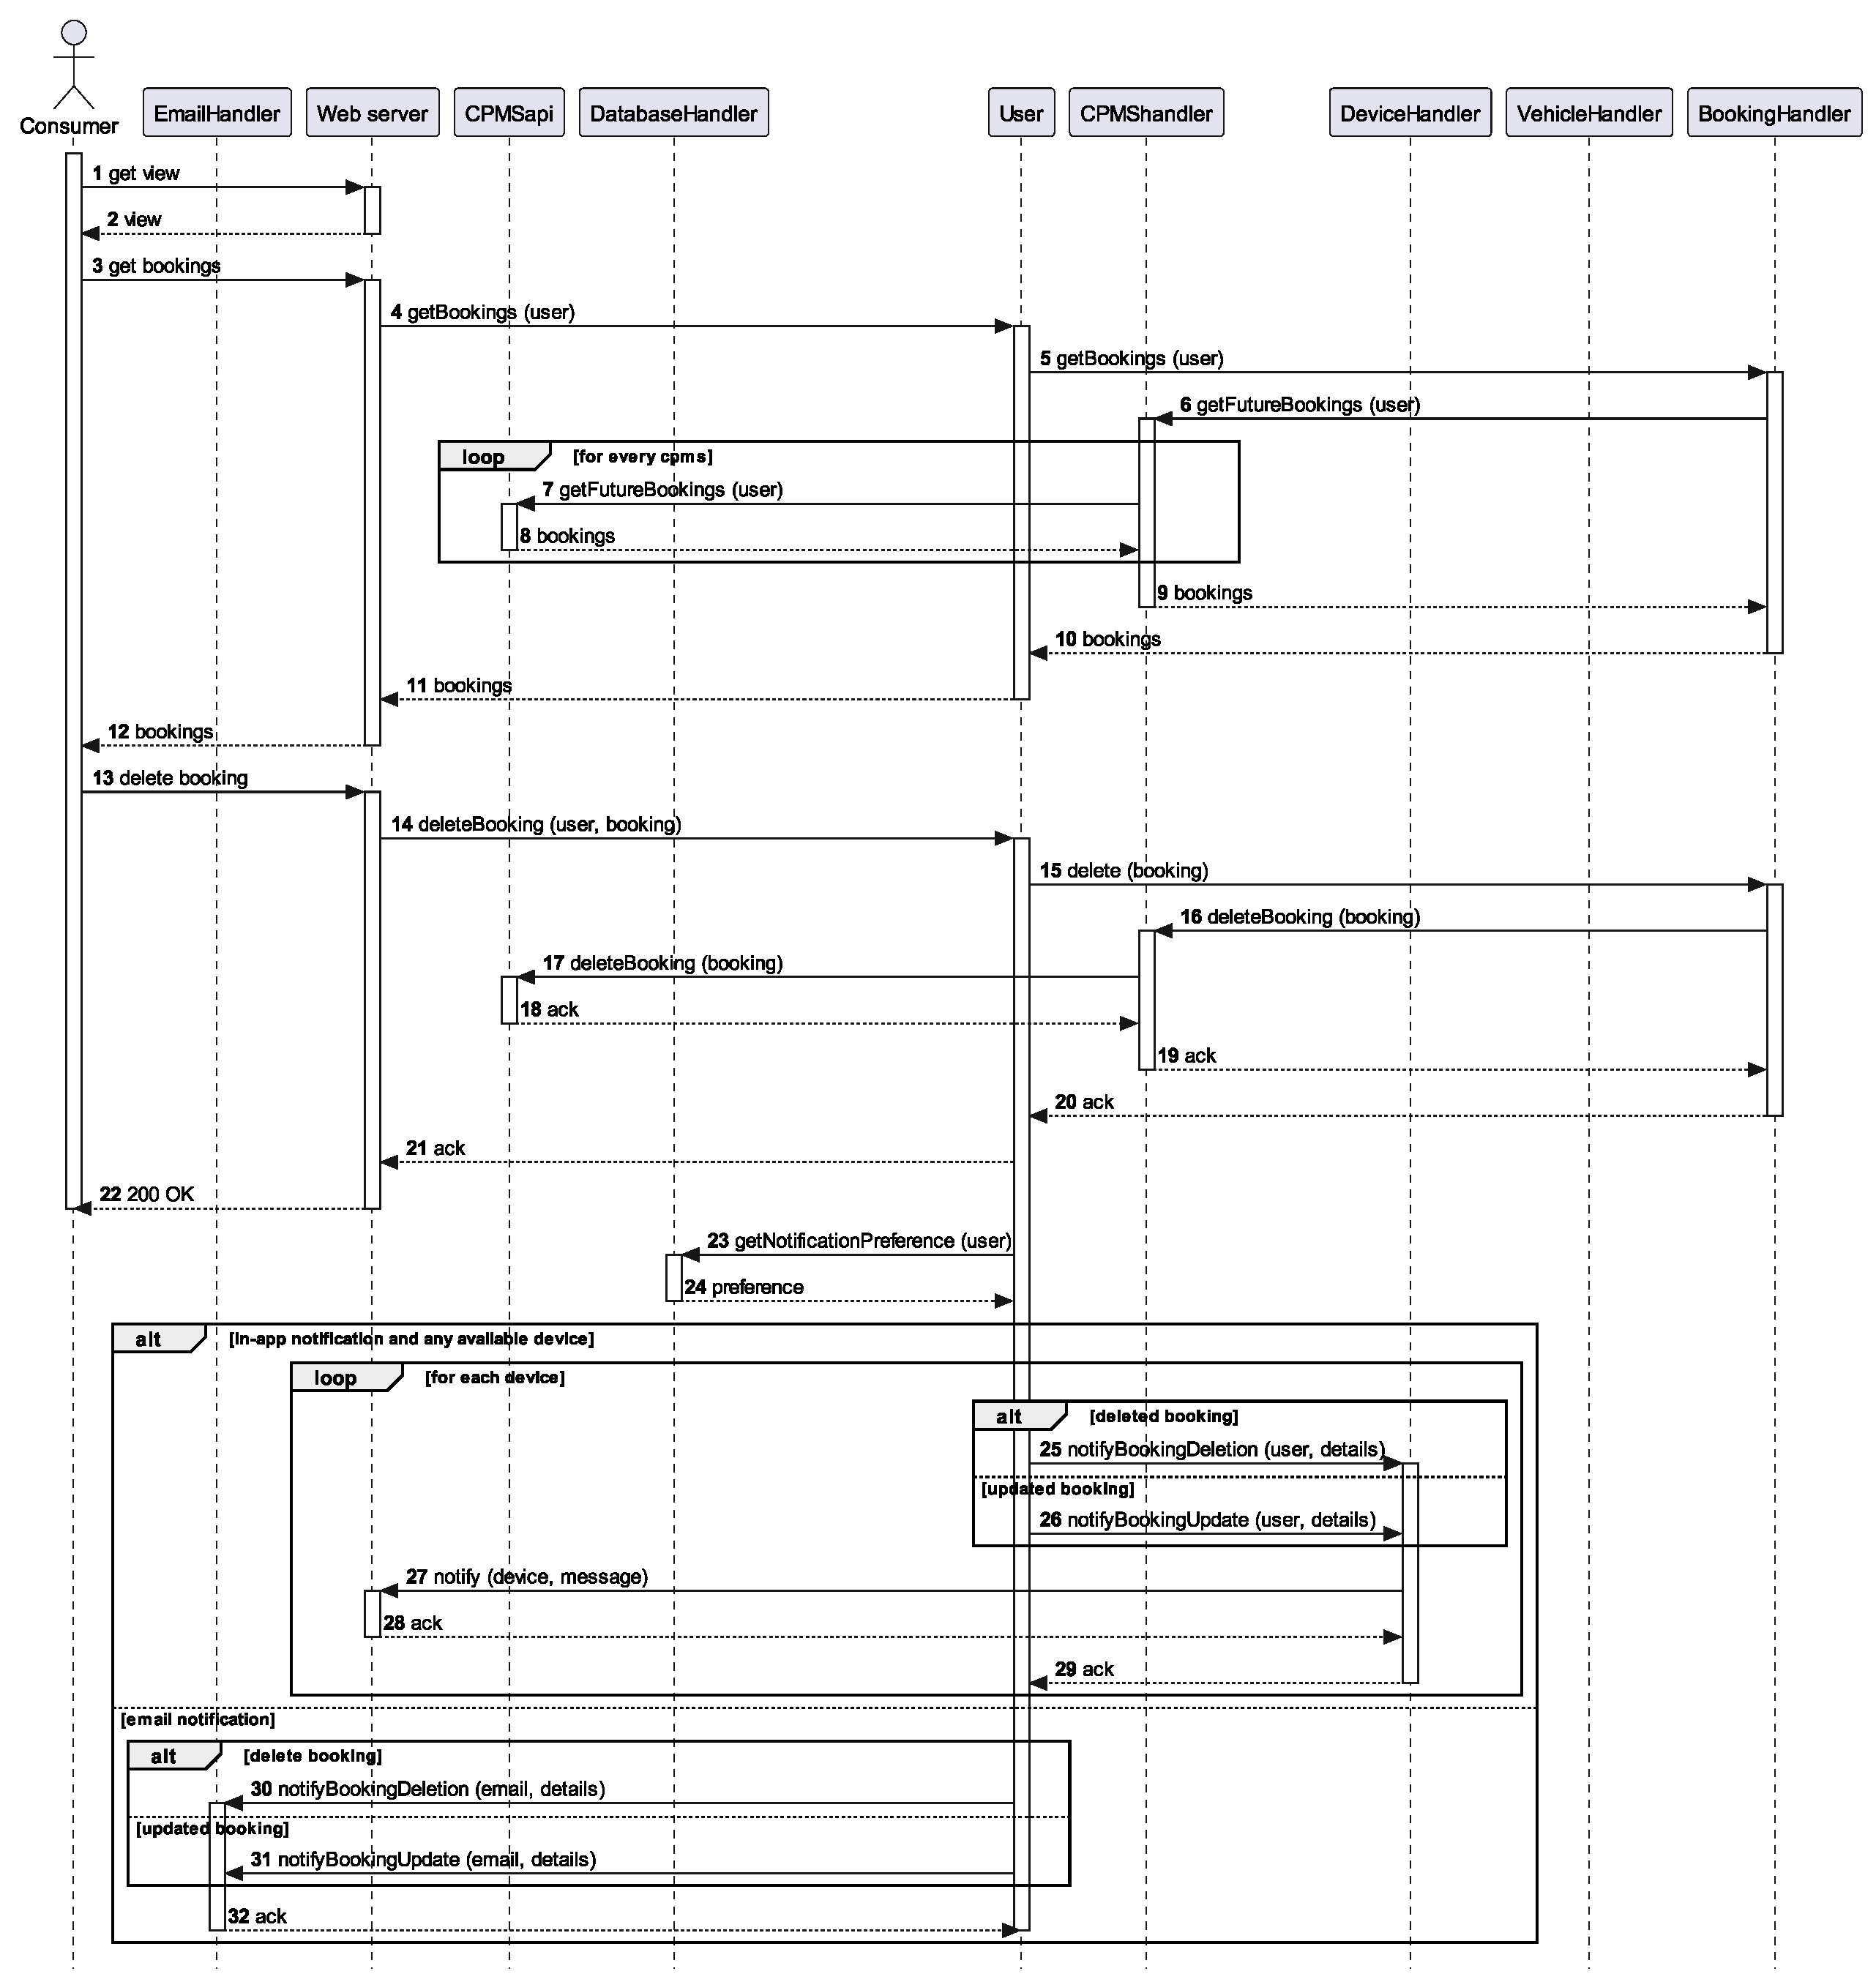
\includegraphics[width=\columnwidth]{./images/sequences/emsp/book_delete}
    \caption{the user removes a booked charge.}
\end{figure}

\pagebreak

\paragraph{Pay for the obtained services} After a charge is completed, the user can pay the charge. If more than one charge needs to be paid, they are aggregated into one single payment.

\begin{figure}[h!]
    \centering
    
\includegraphics[width=\columnwidth]{./images/sequences/emsp/payment}
    \caption{the user pays for the charges.}
\end{figure}

\pagebreak

\paragraph{Editing of a vehicle} The user can edit at any time his/her vehicles. If also the vehicle's certificate is changed, the system automatically updates all future reservations by telling the CPMSs which is the new certificate for the charge.

\begin{figure}[h!]
    \centering
    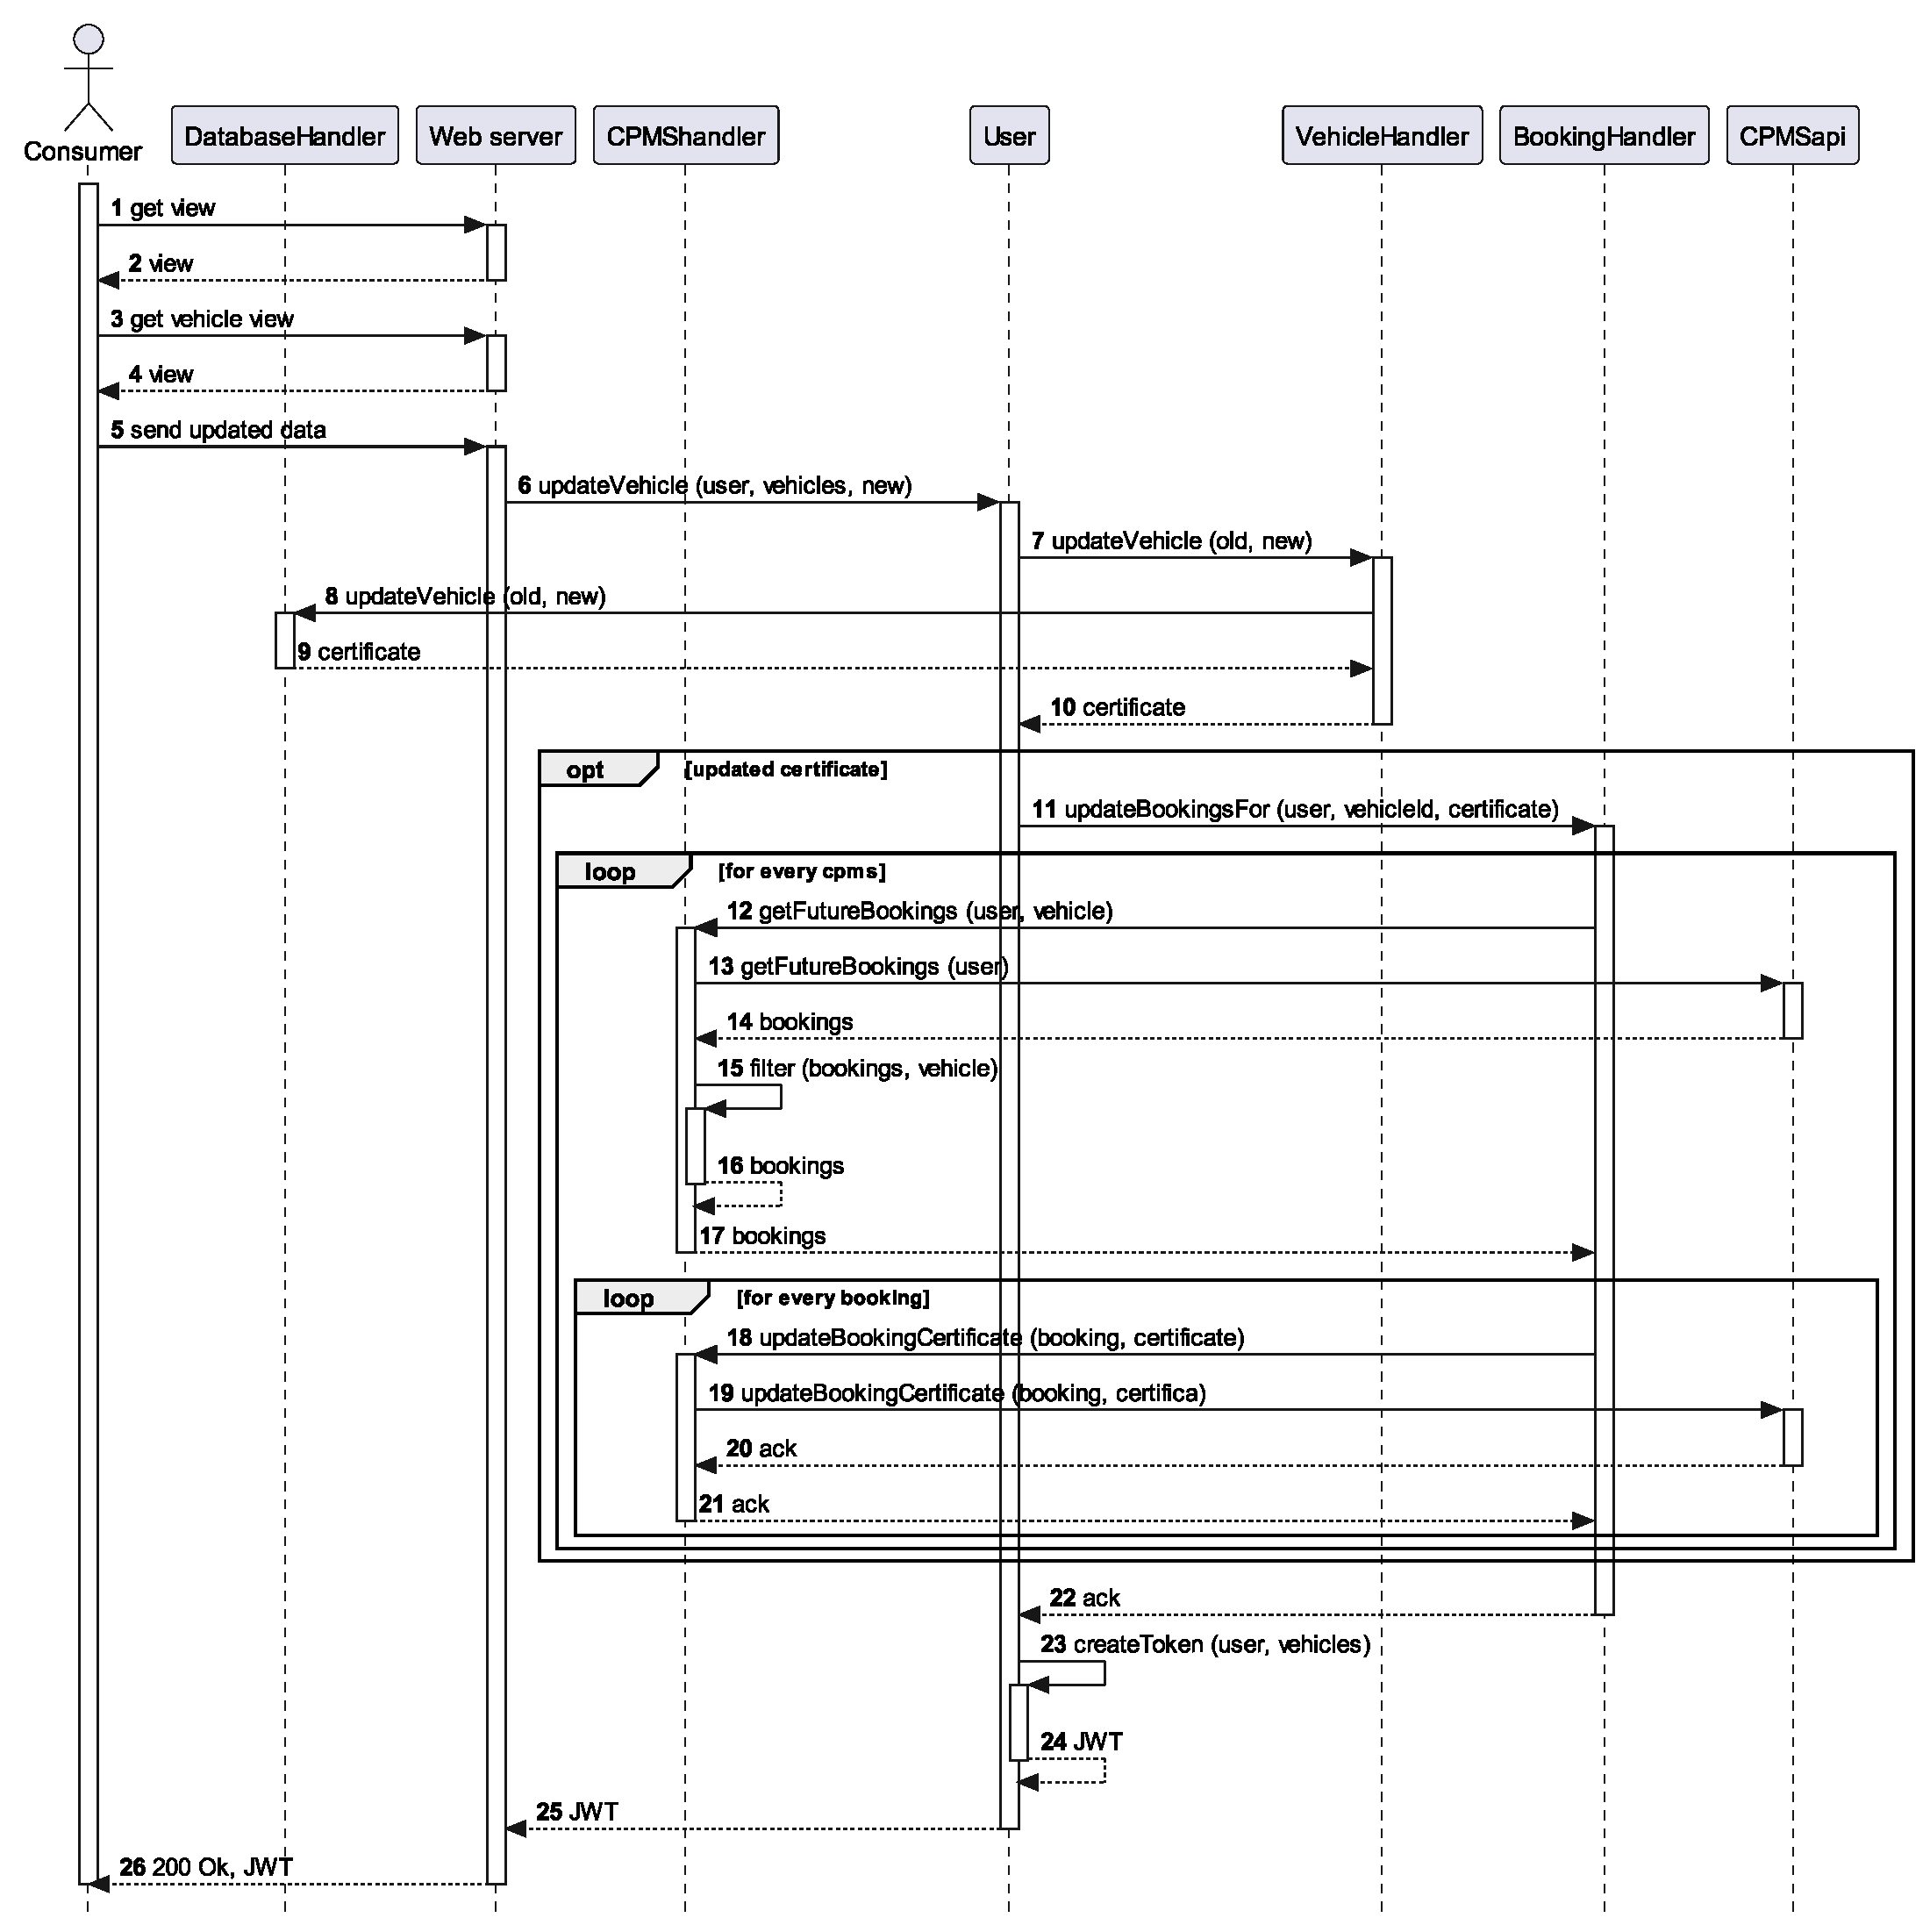
\includegraphics[width=\columnwidth]{./images/sequences/emsp/vehicle_edit}
    \caption{the user edits one of his/her vehicles.}
\end{figure}

\pagebreak

\paragraph{Deletion of a vehicle} The user can delete at any time his/her vehicles. Every time a vehicle is removed, the system automatically deletes all future reservations for that vehicle on every CPMS.

\begin{figure}[h!]
    \centering
    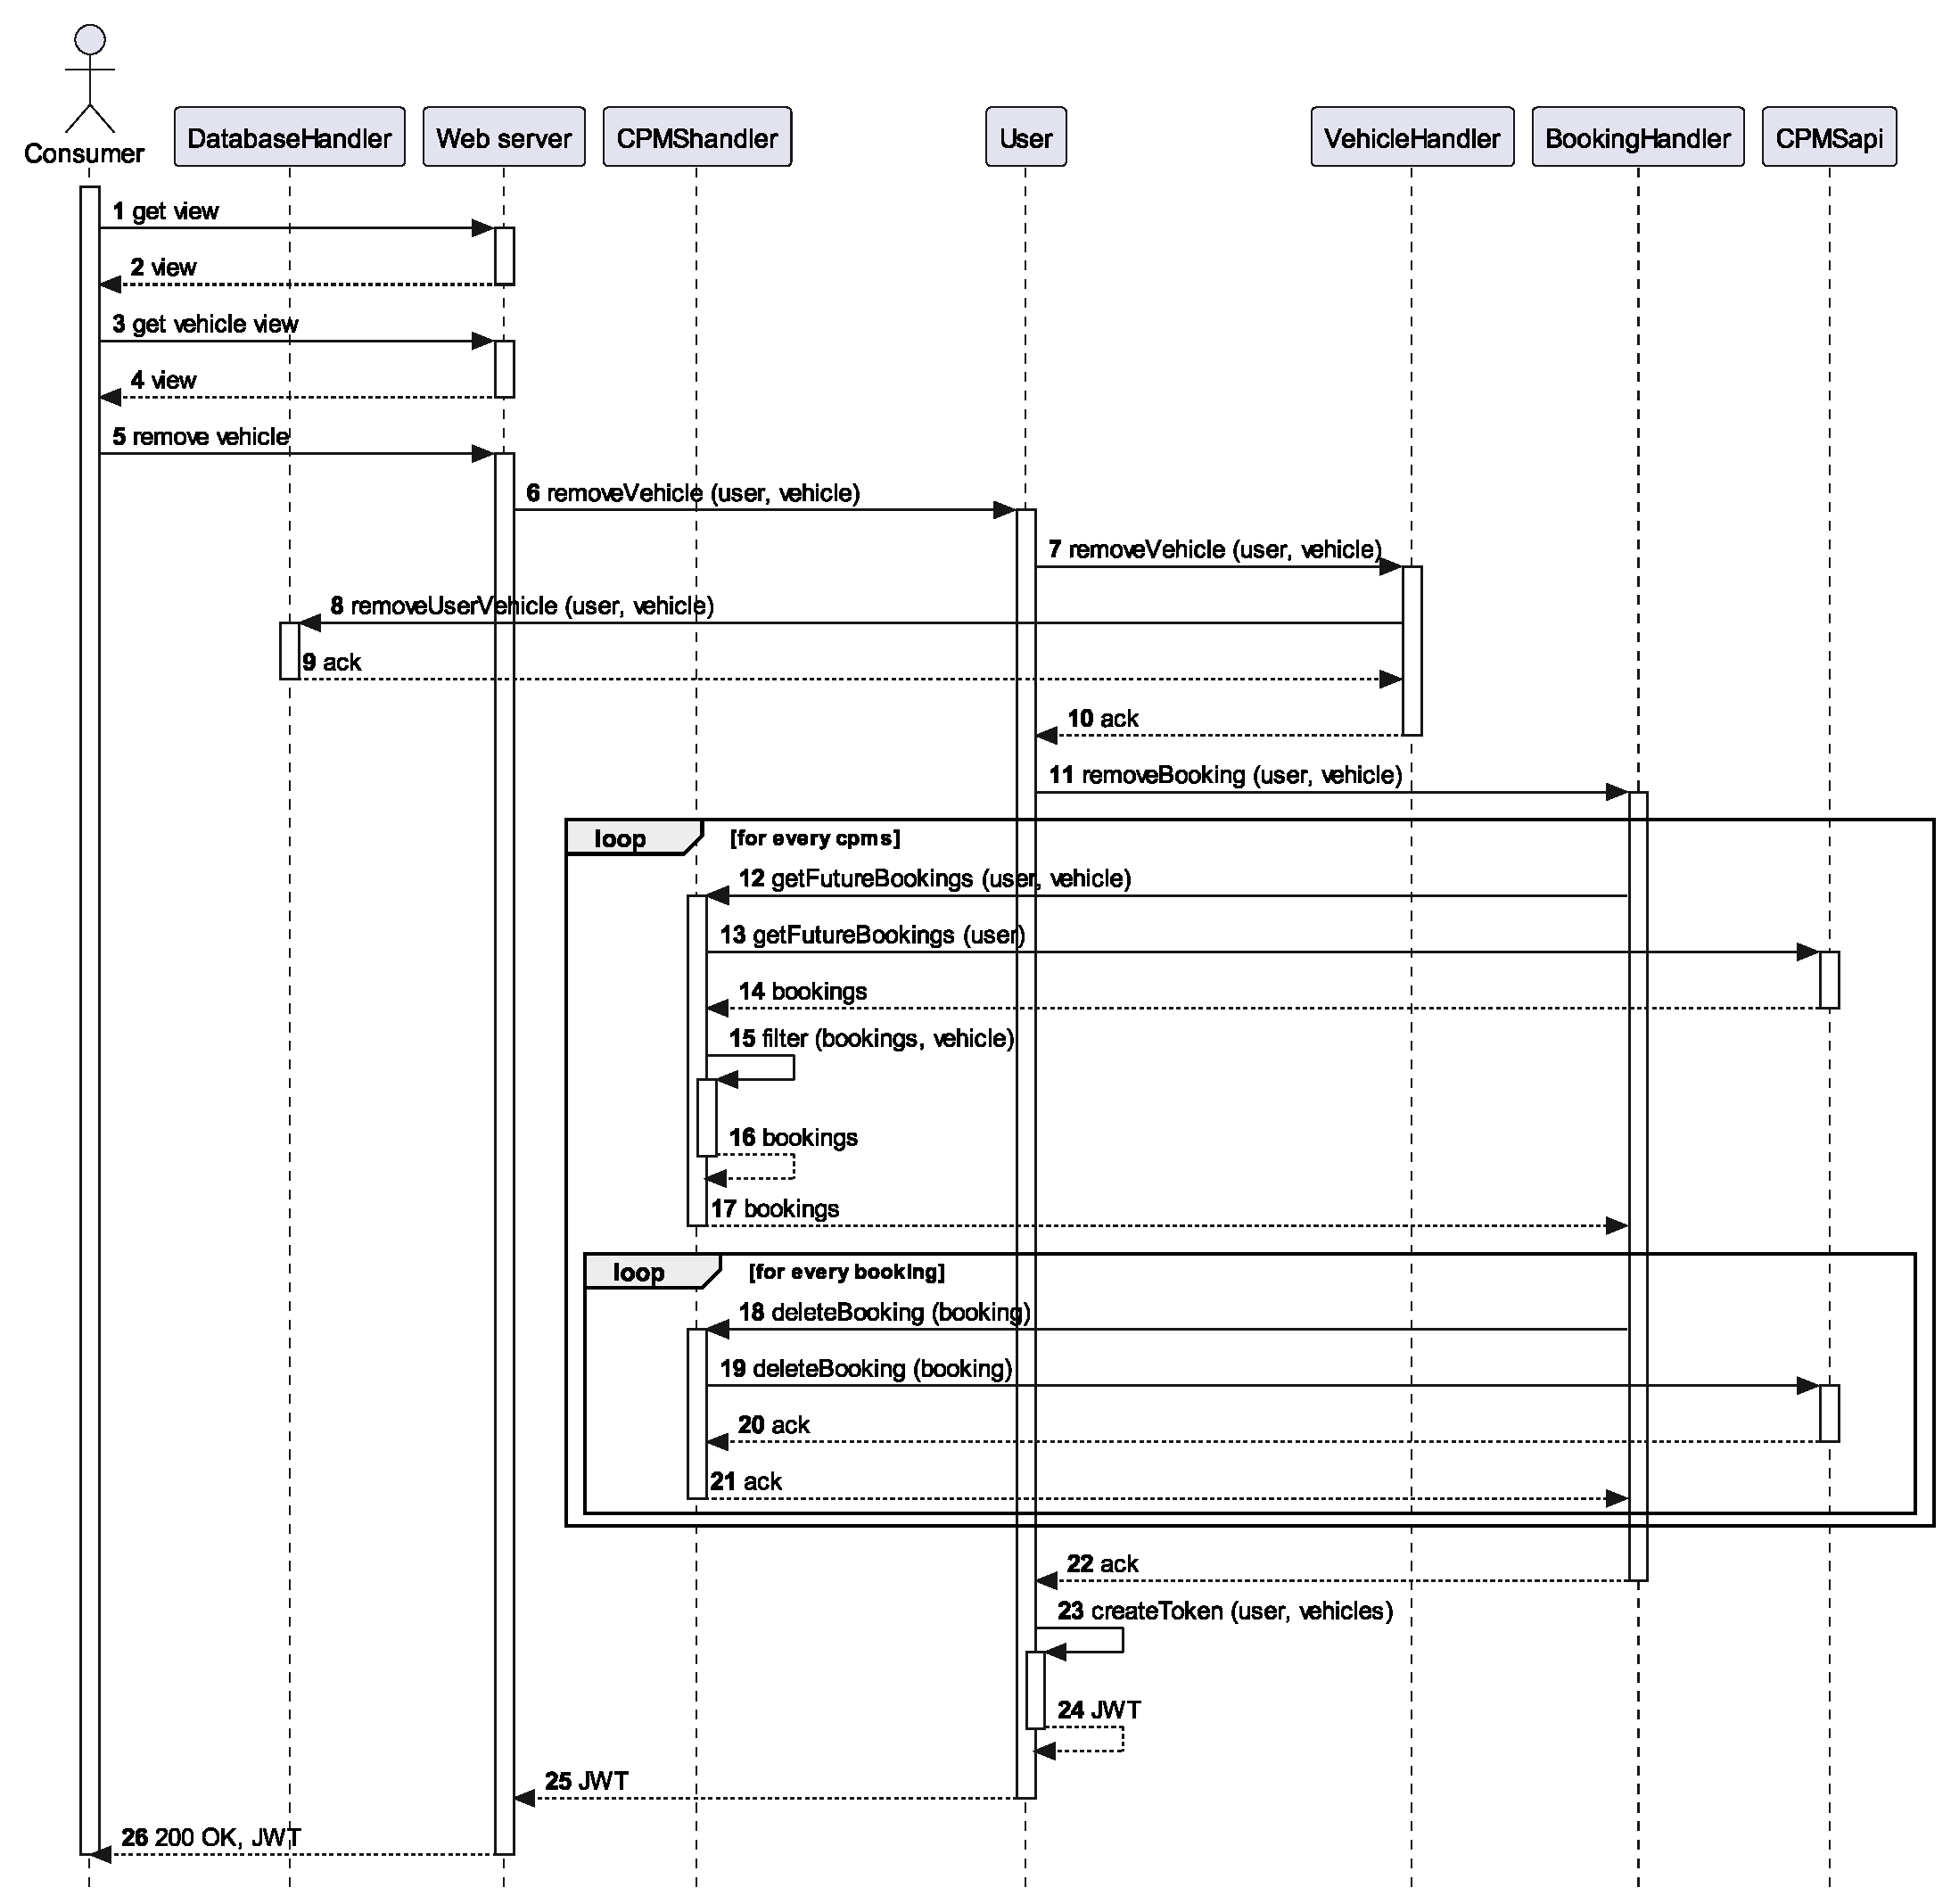
\includegraphics[width=\columnwidth]{./images/sequences/emsp/vehicle_delete}
    \caption{the user removes one of his/her vehicles.}
\end{figure}

\pagebreak

\paragraph{Addition of a new vehicle} The user adds a new vehicle to the system by providing the required data and its certificate.

\begin{figure}[h!]
    \centering
    \includegraphics[width=\columnwidth]{./images/sequences/emsp/vehicle_add}
    \caption{the user adds a new vehicle.}
\end{figure}

\paragraph{Other functions} In the \reference{view:interfaces} section there are some eMSP functions that are not used in these sequence diagrams, in particular:
\begin{itemize}
    \item \texttt{deleteUser (user)} \textit{from} \texttt{UserInterface} \textit{and} \texttt{DatabaseInterface}: if the user doesn't have any pending payment, the system removes all his/her data from the system and all the future bookings.
    \item \texttt{export (user)} \textit{from} \texttt{UserInterface}: allows the user to export all his/her data collected by the eMSP and the CPMS, according to the GDPR.
    \item \texttt{getAllBookings (user)} \textit{from} \texttt{CPMSinterface} \textit{and} \texttt{UserInterface}: retrieves all the booking for that user on every connected CPMS.
    \item \texttt{resetPassword (user)} \textit{and} \texttt{resetPassword (id, link)} \textit{from} \texttt{UserInterface} \textit{and} \linebreak \texttt{DatabaseInterface}: these two methods allow the user to reset his/her access password by proving the email address used for logging in. The system sends the user an email with the link for changing it.
    \item \texttt{updateUser (user, newData)} \textit{from} \texttt{UserInterface}: allows the user to update all his/her data, including the password.
    \item \texttt{updateDevice (user, device)} \textit{from} \texttt{DeviceInterface} \textit{and} \texttt{DatabaseInterface}: even if it's not presented in the diagrams, it's called on every request for keeping updated the list of devices of the user, which are automatically cleaned up after a while if unused.
    \item \texttt{handshake (cpms)} \textit{from} \texttt{CPMSinterface} \textit{and} \texttt{addCPMS (cpms)} \textit{and} \texttt{getInfo ()}\footnote{This function (\texttt{getInfo ()}) allows to retrieve all the eMSP's information that need to be sent to the newly connected CPMS.} \textit{from} \linebreak \texttt{DatabaseInterface}: these functions allow the system to conncet to a newly discovered CPMS and to store it's information into the database.
    \item \texttt{getCPMS (id)} \textit{and} \texttt{getCPMSs ()} \textit{from} \texttt{DatabaseInterface}: allow retrieving data about a specific CPMS or about every connected one.
\end{itemize}

\vfill

\pagebreak

\subsection{CPMS}

\paragraph{Login} The user logs into the system, which recognizes him/her and sends back a signed JWT for future actions on the system, like monitor stations. This token is properly checked on every request by the web server. 

After authentication, the home page view is sent, then asynchronous sub-processes are run to fetch and send information about stations and DSOs. This information is sent in the form of JSON files.

From login until logout (or until a certain inactivity time has elapsed) the \texttt{Web Server} process will not end. 

\begin{figure}[h!]
    \centering
    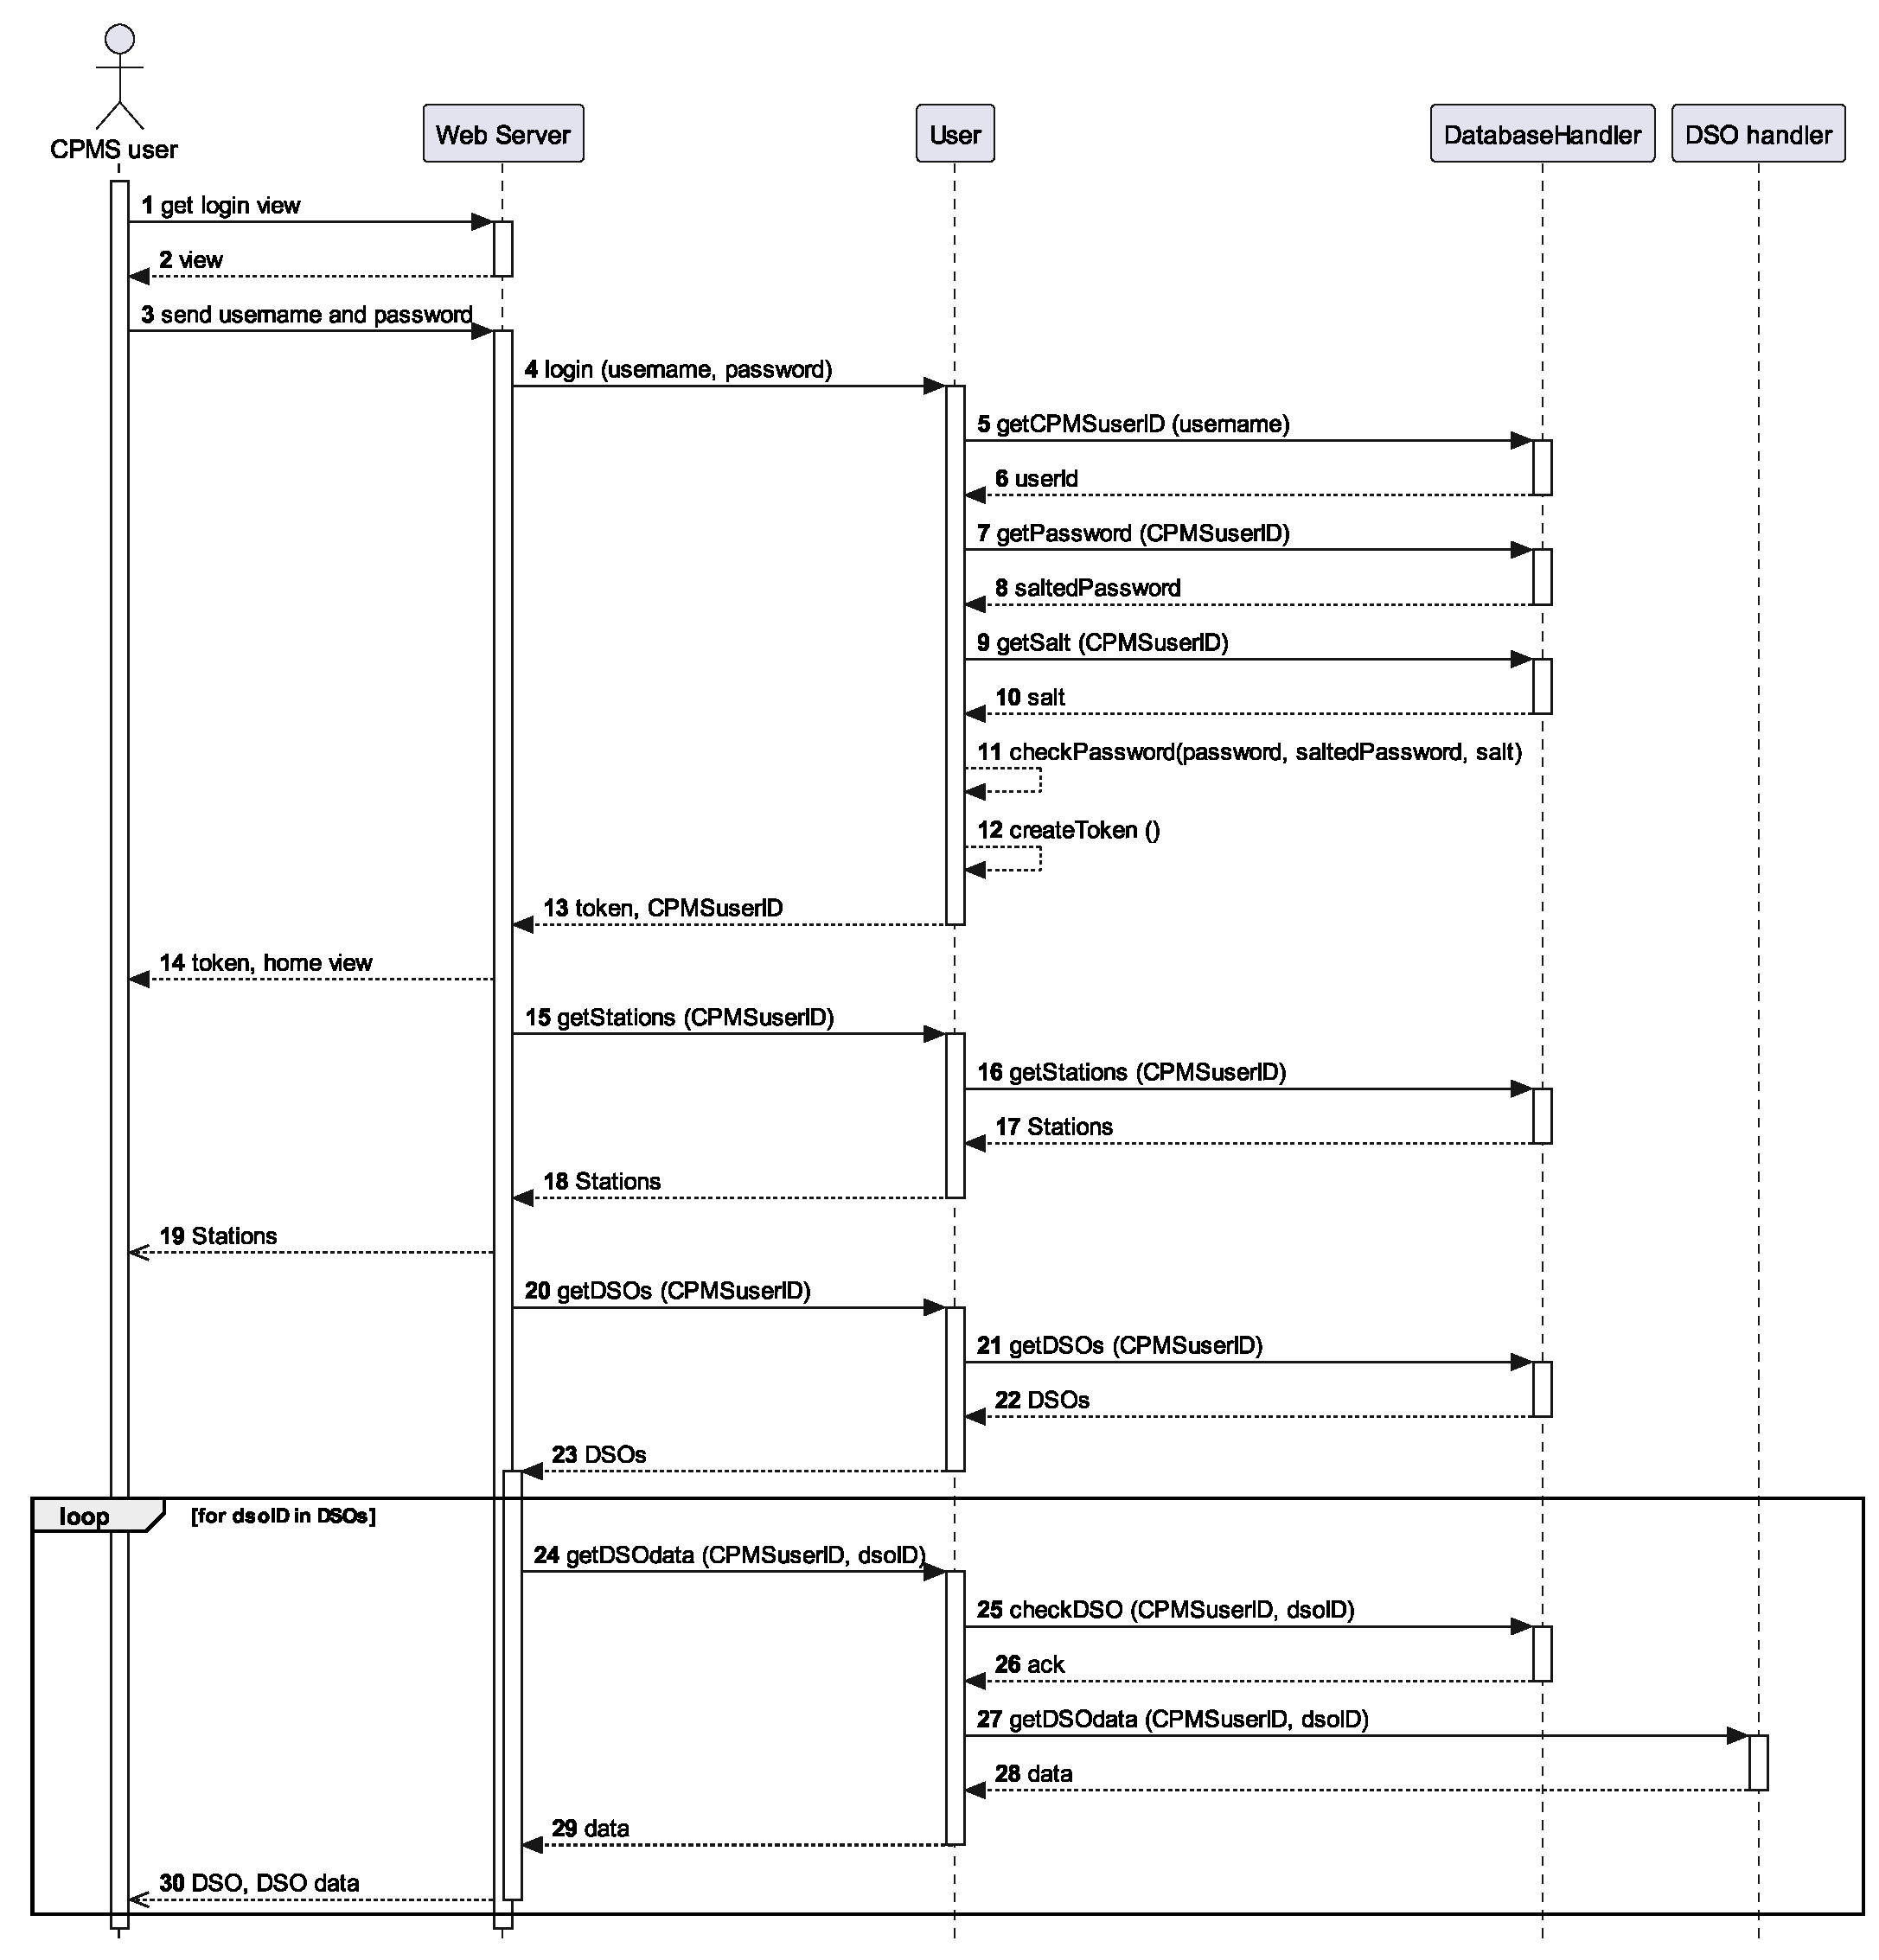
\includegraphics[width=\columnwidth]{./images/sequences/cpms/login}
    \caption{the user logs into the CPMS website.}
\end{figure}

\pagebreak

\paragraph{Monitoring a station} In the \doublequotes{Station} view users can monitor the situation inside stations. Until they leave the page, the \texttt{Web Server} will run an asynchronous periodical loop to fetch new information to send in JSON files. 

\begin{figure}[h!]
    \centering
    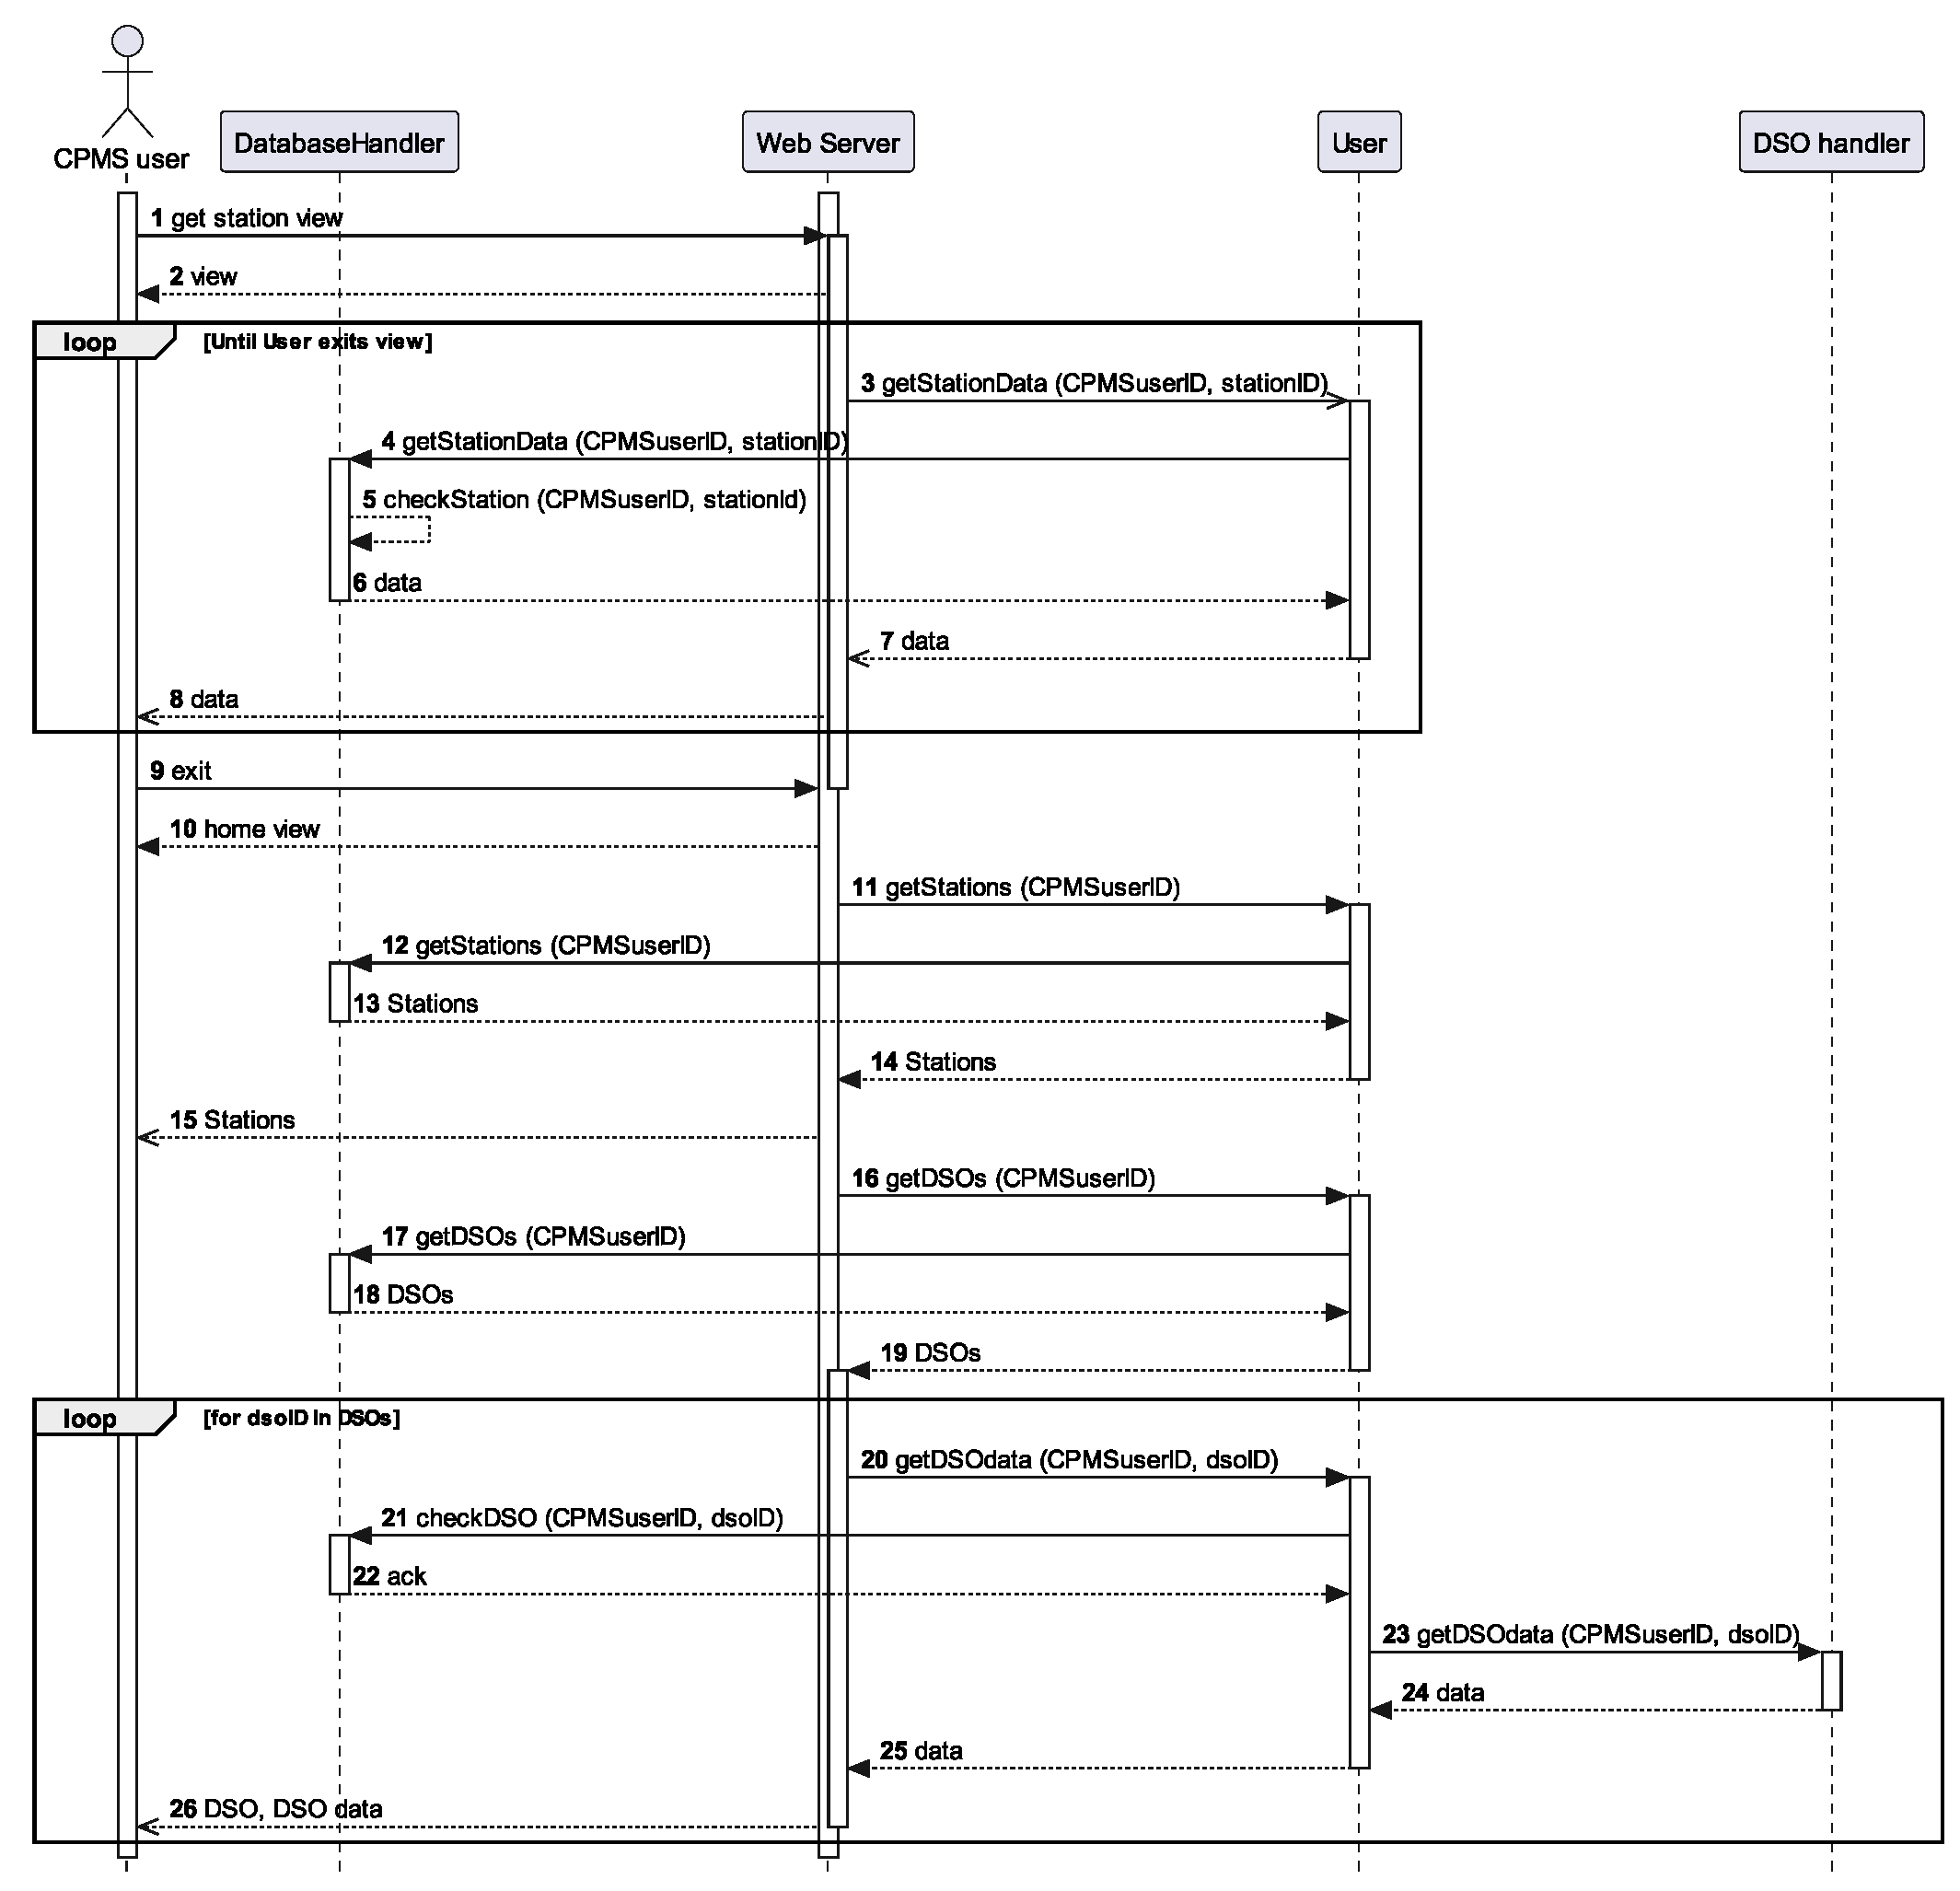
\includegraphics[width=\columnwidth]{./images/sequences/cpms/monitor}
    \caption{the user selects a station to view, then goes back to the home page.}
\end{figure}

\pagebreak

\paragraph{Activating automatic energy mix} From a \doublequotes{Station} view, the user selects \doublequotes{Automatic Mix choice}, then decides to log out. Since \doublequotes{automatic mix} is activated, the \texttt{ChargingStation} process enters a loop until this option is deactivated. In this loop, it periodically fetches information from sensors, decides what the best energy mix is, then waits some time.

\begin{figure}[h!]
    \centering
    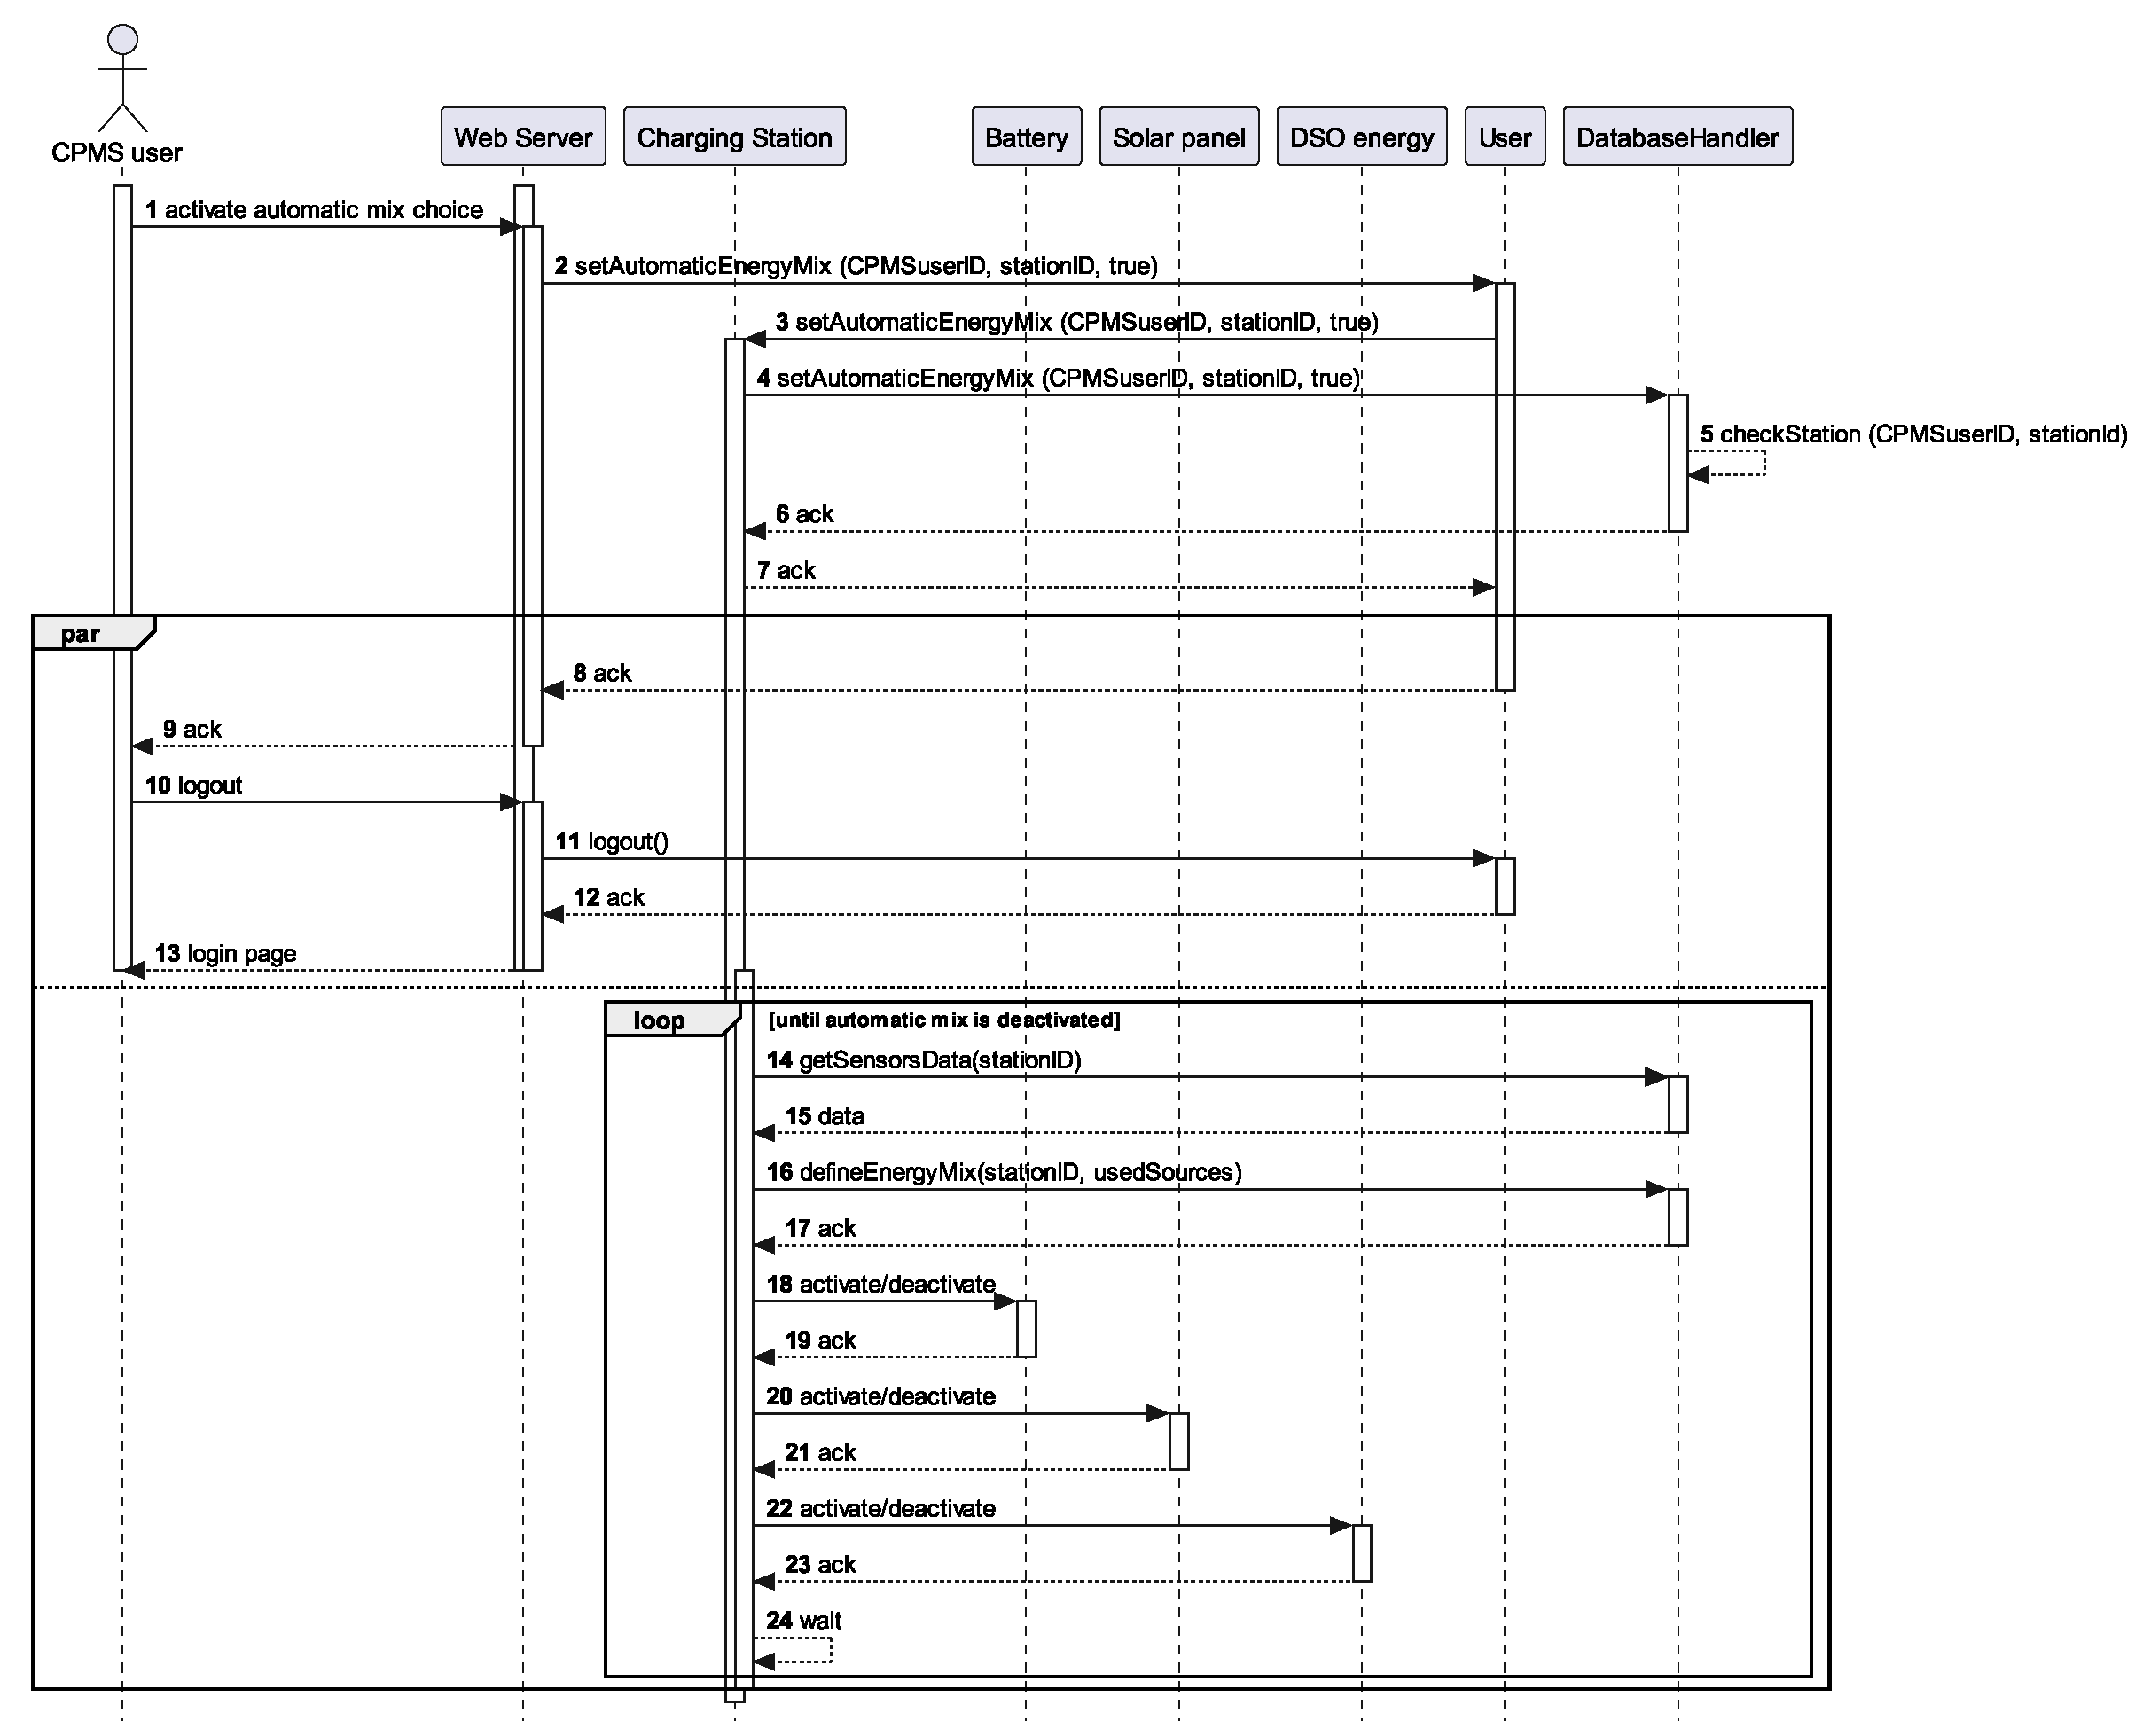
\includegraphics[width=\columnwidth]{./images/sequences/cpms/energyMix}
    \caption{the user activates automatic mix choice, then logs out of the website.}
\end{figure}

\pagebreak

\paragraph{DSO choice} From a \doublequotes{Station} view, the user selects \doublequotes{Automatic DSO choice}, then selects another DSO, ending the automatic choice. Since \doublequotes{automatic DSO choice} is activated, the \texttt{ChargingStation} process enters a loop until this option is deactivated. In this loop, it periodically fetches information from DSOs, decides what the best price is, selects that DSO, then waits some time.

\begin{figure}[h!]
    \centering
    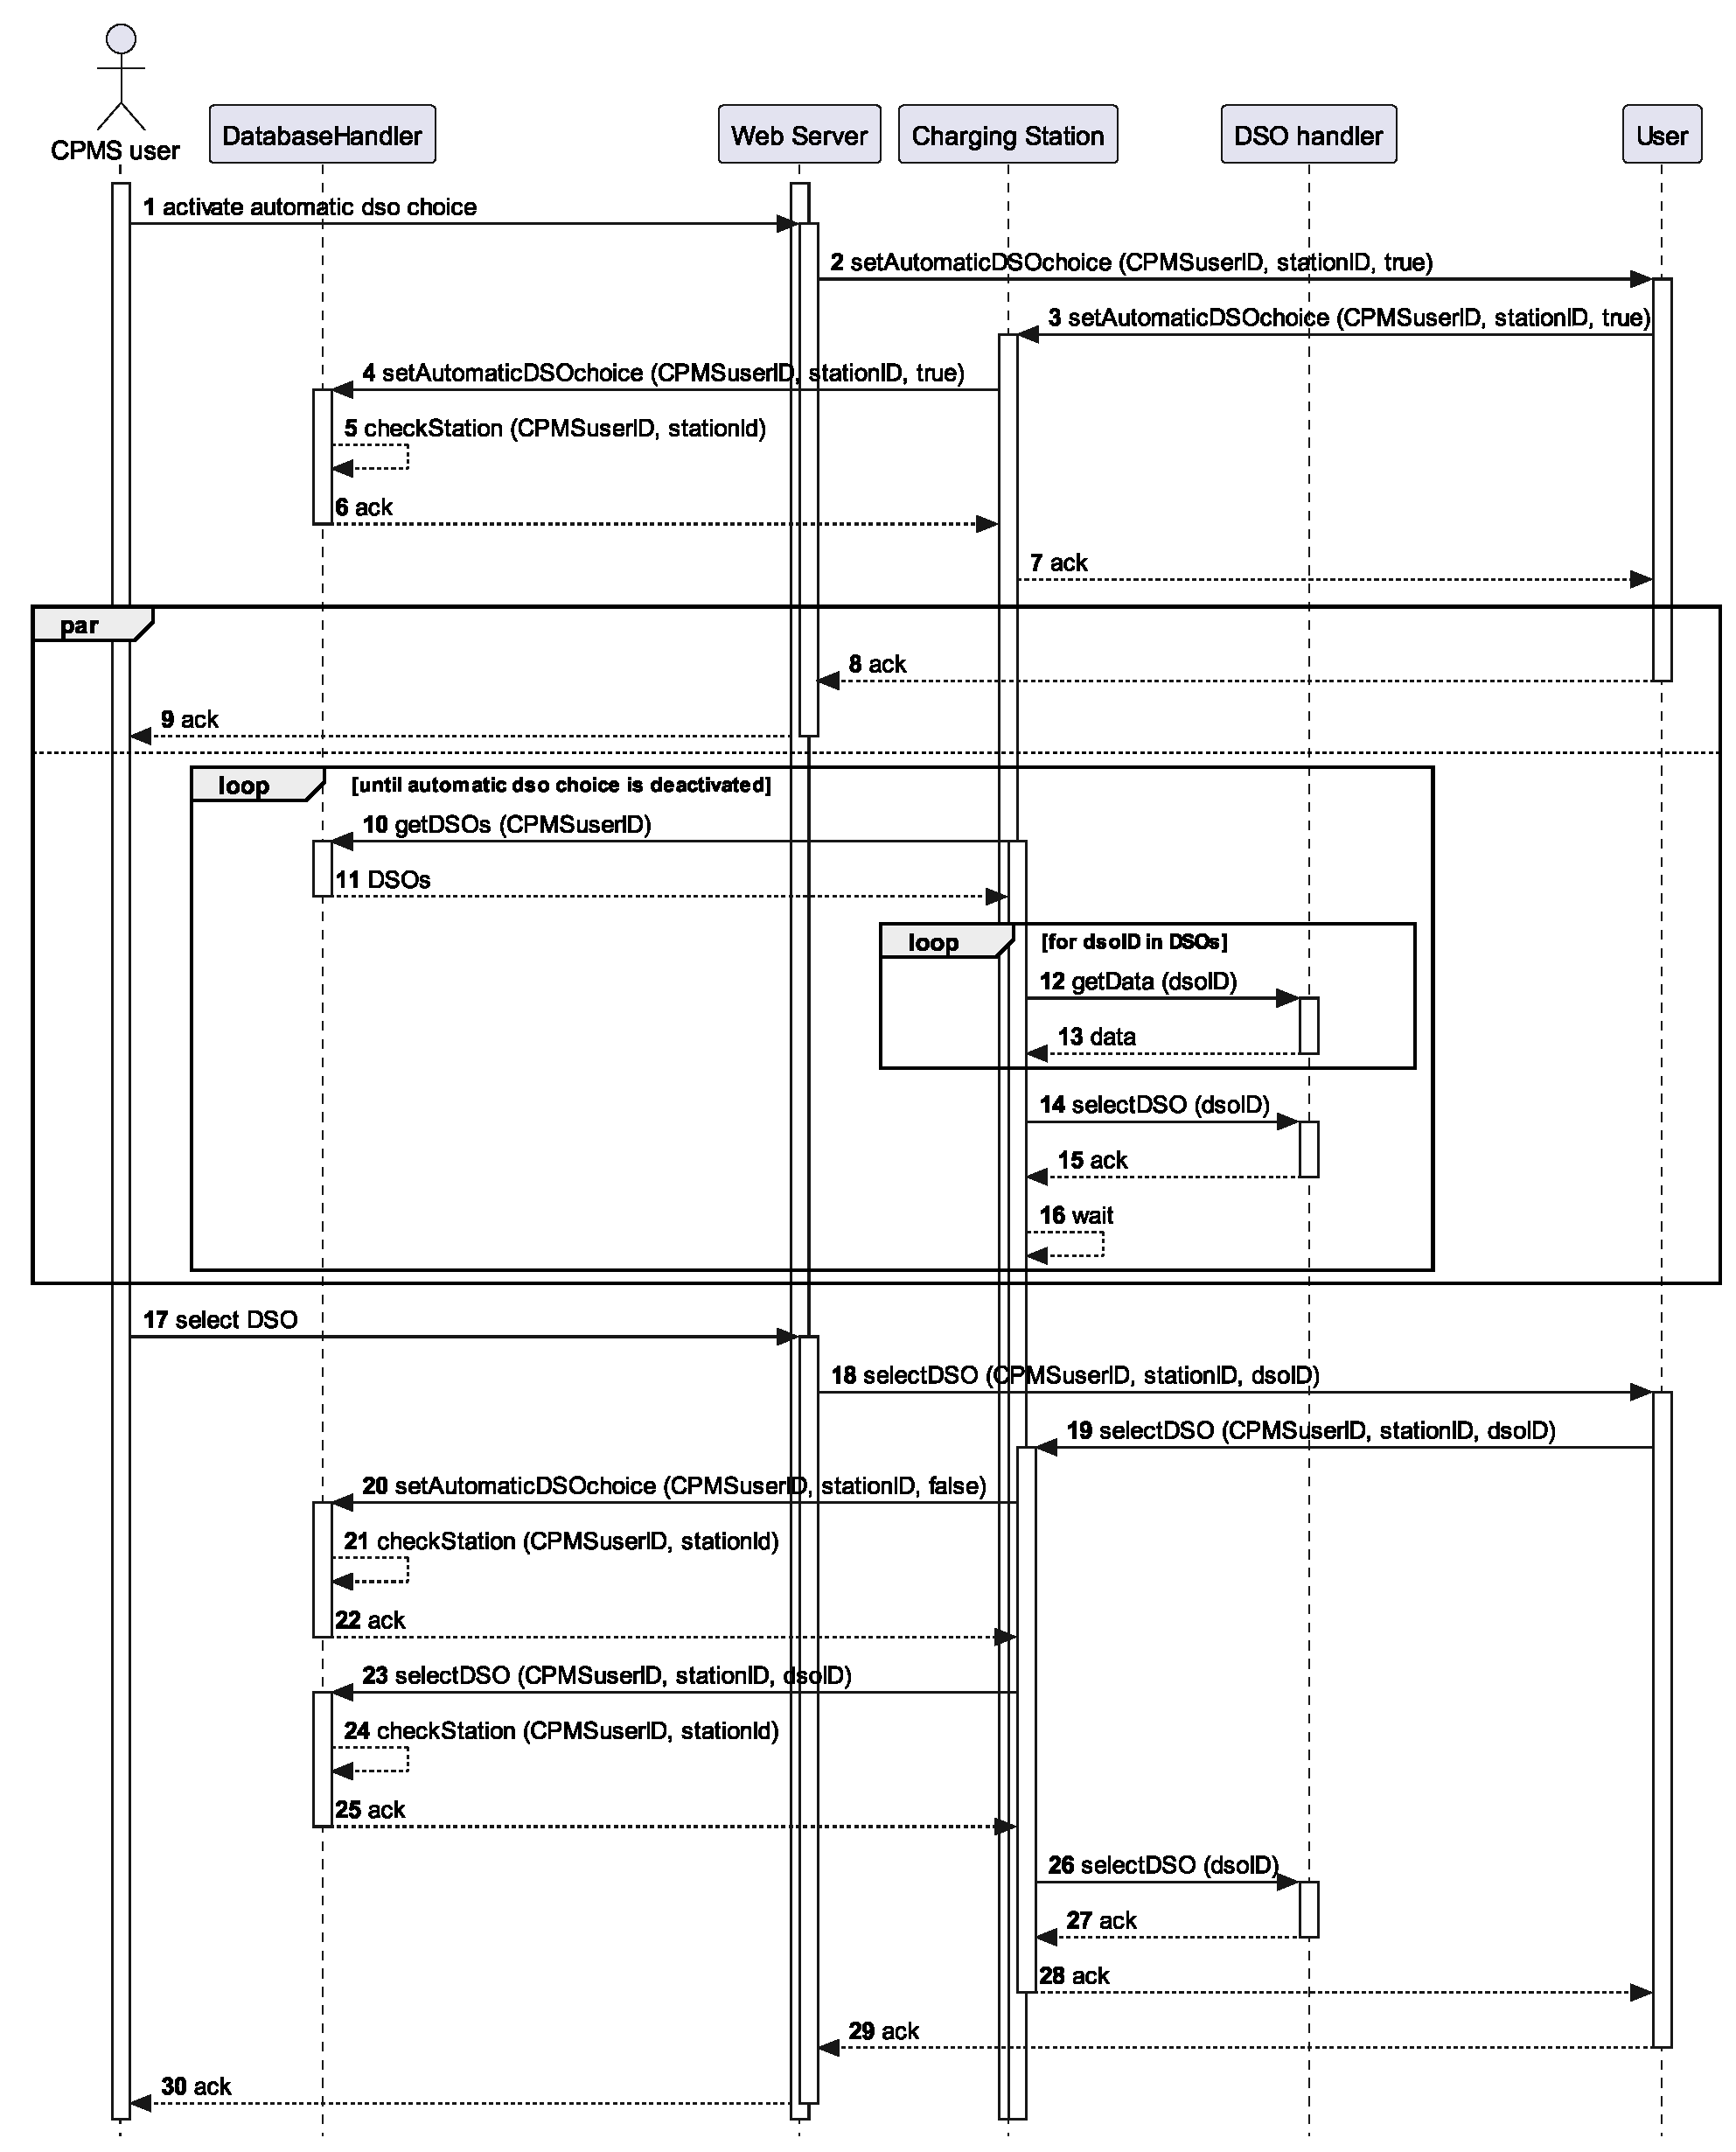
\includegraphics[width=\columnwidth]{./images/sequences/cpms/dso}
    \caption{the user activates automatic DSO choice, then deactivates it by selecting a specific DSO.}
\end{figure}

\pagebreak

\paragraph{Create a new special offer} The user enters the \doublequotes{Offer} view and creates a new special offer.

\begin{figure}[h!]
    \centering
    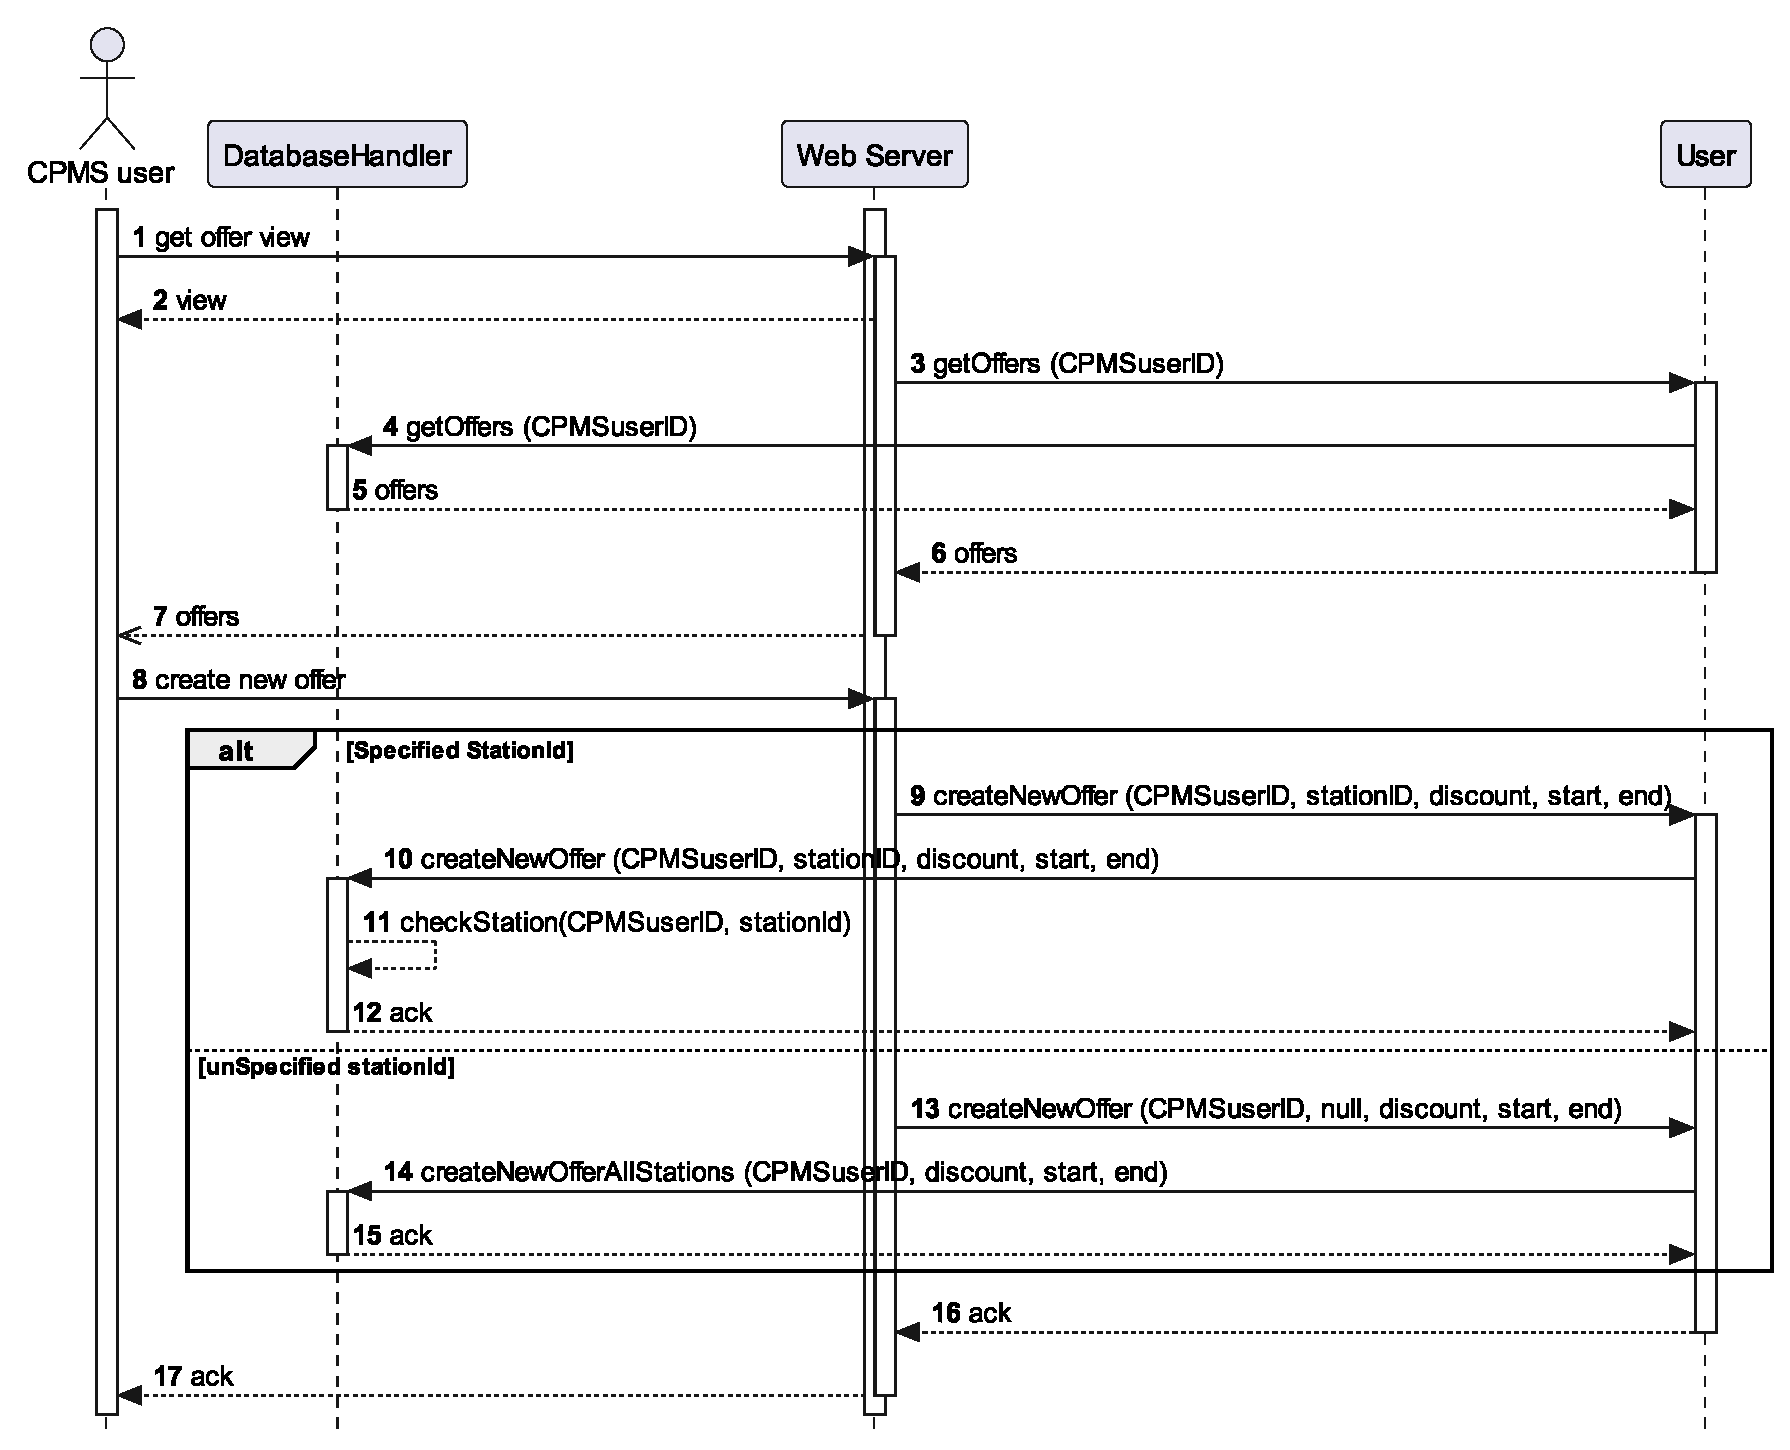
\includegraphics[width=\columnwidth]{./images/sequences/cpms/offers}
    \caption{the user creates a new special offer.}
\end{figure}

\paragraph{Other functions} The CPMS system allows for other actions to occur, but they are not depicted here because they are fairly basic, and their diagram can be better described with words. Every notification to the eMSP is sent through the \texttt{sendNotification (eMSP\_ID, eMSPuserID, message)} function of the \texttt{eMSPinterface}. eMSP users are allowed to pay the charge at the charging station, therefore \texttt{ChargingColumn} can access the \texttt{PaymentInterface} in order to use the function \texttt{payCharge (eMSPuserID, paymentData)}. eMSP add, delete, update and query bookings through the use of the various \doublequotes{Booking} functions of the \texttt{BookingInterface} and the \texttt{DatabaseInterface}. eMSPs are added to the database though the function \texttt{add\_eMSP (eMSP)} called by the eRoamingHandler.

\pagebreak

\section{Selected architectural styles and patterns}

Here are presented all the design patterns that have been chosen for building up the two systems, which are very similar in this aspect.

\subsection{Three-tier architecture}

Both the eMSP and the CPMS present a three-tier architecture. This is because it helps to divide the local functions of every component into three different \doublequotes{classes} (presentation, business and data) which have different duties. The presentation layer is in charge of directly answering the user's requests, activating the required components in the backend, and collecting the final answer. The data layer is in charge of keeping organized all the data of the system. Finally, the business is the logical core of the system, indeed it provides the needed answers to the frontend by indirectly analyzing the requests from the client and picking and processing the required data from the data layer.

\subsection{Microservice architecture}

Both the eMSP and the CPMS present a microservice architecture. This design decision has been taken because it allows the system to be more resilient, to be able to scale better (e.g. duplicating the bottleneck components) and it can also be developed, updated, and tested by different teams, allowing a faster startup.

\subsection{Containerized architecture}

Both the eMSP and the CPMS present a containerized business layer. For providing even stronger security and resilience to failures, all those components are containerized, which means that all run on a different \doublequotes{virtual} environment, without the knowledge of the whole system on which they are running. Thanks to the use of a Kubernetes service, it's possible to orchestrate multiple machines in order to proactively react to the traffic to the service and easily update components. This can be done thanks to the volatile nature of the containers, which can be brought up and down and updated in a really easy way.

\subsection{Database-centric architecture}

Both the eMSP and the CPMS present a database-centric architecture. This implies that every component relies on the database for obtaining data and processing information. In case of failures of components, they can be restarted without any loss since all the information is stored in the database, which, itself, is a replicated piece of software.

\subsection{RESTful architecture}

Both the eMSP and the CPMS present a RESTful architecture. This is especially true in the client-server relation since the client only asks the server for HTML, CSS and JavaScript files for correctly visualizing pages (which is not required in the case of the eMSP's mobile application) and then queries the server through standard HTTP requests for the required data, providing a JWT at every request for being recognized.

\subsection{Observer design pattern}

Components in the CPMS system can implement the observer pattern: \texttt{ChargingColumn} and \texttt{EnergySource} offer through their interfaces the \texttt{addObserver (observer)} function, \texttt{ChargingStation} can then add observers to them. These observers are used to prevent in-station batteries from passing a certain charge level or to send a notification when the user's car's charge ends.

    \chapter{User Interface Design} \label{ui}

This third chapter is about the frontend interfaces the users will use for accessing and interacting with the two systems. For every system, there is a brief  presentation of all the main interfaces they are composed of, and then, thanks to the use of flow diagrams, the navigation flow is presented.\medskip

These represent only the interfaces used by the end users of the two systems, the pages for the system administrators are not presented here, since their views are similar to these or consist only of a list of employees with the possibility to add or remove them (which is especially true in the CPMS).\medskip

Moreover, these interfaces are presented only in day/light mode for better readability, but in real-case scenarios, they adapt to the user's (or browser's) preferred theme, so they come also with a night/dark mode.

\section{eMSP}

The eMSP is the system that interacts with the end user of the whole system: the consumer. In this section, the only presented mockups are the ones of the mobile application. The ones available from the browser are the same, with the only difference being that in the case of a landscape design (which is more common on desktop/personal computers), the elements of the interfaces are organized in a slightly different way to better adapt to the display.

\subsection{Interfaces design}

Here are presented all the mockups of the pages of the mobile application of the eMSP. The mobile application is available on all the main application stores for mobile phones available nowadays, like \textit{App Store} (Apple), \textit{Google Play Store} (Google), and \textit{AppGallery} (Huawei). The browser version is slightly different since it's usually used on a landscape device.

\pagebreak

\paragraph{Login and signup} When the user first opens the application or the personal area of the eMSP website, he is prompted to log into the application, but if the user doesn't still have an account, there is the possibility to go to the signup page (or registration page) where he is asked to insert all of his data. The interface also offers the possibility to display (or to hide) the password and to display a date picker to easily insert the birthdate.

\begin{figure}[h!]
    \centering
    \begin{minipage}{0.49\textwidth}
        \centering
        \fbox{\includegraphics[width=\textwidth]{images/mockups/emsp/signup_login/login}}
        \caption{login page.}
    \end{minipage}
    \hfill
    \begin{minipage}{0.49\textwidth}
        \centering
        \fbox{\includegraphics[width=\textwidth]{images/mockups/emsp/signup_login/signup}}
        \caption{signup (registration) page.}
    \end{minipage}
\end{figure}

\pagebreak

\paragraph{Post registration actions} After the uses registers to the application, the system sends him/her an email with a link for activating the account. Once the user clicks on it, s/he is sent to the login page where a popup tells the user that his/her registration ended up successfully. After closing the banner, the user can log into the application, and since it's the first login, the home page is displayed and s/he is asked whether to use any logged-in device for sending notifications or the associated email address.

\begin{figure}[h!]
    \begin{minipage}{0.49\textwidth}
        \centering
        \fbox{\includegraphics[width=\textwidth]{images/mockups/emsp/signup_login/confirmed}}
        \caption{successful registration message.}
    \end{minipage}
    \hfill
    \begin{minipage}{0.49\textwidth}
        \centering
        \fbox{\includegraphics[width=\textwidth]{images/mockups/emsp/signup_login/notification}}
        \caption{first choice of the notification method.}
    \end{minipage}
\end{figure}

\pagebreak

\paragraph{Home page} The home page is the center of the application. From here the user can reach his profile with all the details, the map for booking charges, the history of his charges, and the future ones (which also appear on the home page, as shown in \figureref{figure:ui:emsp:home}), and, if any, a button for paying all the unpaid charges.

\begin{figure}[h!]
    \begin{minipage}{0.49\textwidth}
        \centering
        \fbox{\includegraphics[width=\textwidth]{images/mockups/emsp/homepage_profile/home}}
        \caption{home page with no bookings.}
    \end{minipage}
    \hfill
    \begin{minipage}{0.49\textwidth}
        \centering
        \fbox{\includegraphics[width=\textwidth]{images/mockups/emsp/homepage_profile/charges}}
        \caption{home page with bookings.}
        \label{figure:ui:emsp:home}
    \end{minipage}
\end{figure}

\pagebreak

\paragraph{User's profile} From this page, the user can see all the data s/he uploaded to the system and can update, download, and delete it. Moreover, from this point, the user can log out from the system, change the preferred notification method and reach his/her vehicles page.

\begin{figure}[h!]
    \begin{minipage}{0.49\textwidth}
        \centering
        \fbox{\includegraphics[width=0.71\textwidth]{images/mockups/emsp/homepage_profile/profile}}
        \caption{profile page with all the details.}
    \end{minipage}
    \hfill
    \begin{minipage}{0.49\textwidth}
        \centering
        \fbox{\includegraphics[width=0.71\textwidth]{images/mockups/emsp/homepage_profile/update}}
        \caption{page for profile update.}
    \end{minipage}
\end{figure}
\begin{figure}[h!]
    \centering
    \begin{minipage}{0.49\textwidth}
        \centering
        \fbox{\includegraphics[width=0.71\textwidth]{images/mockups/emsp/homepage_profile/notification}}
    \end{minipage}
    \caption{notification preference change on user's profile.}
\end{figure}

\pagebreak

\paragraph{Stations lookup: map view} The map view allows the user to see all the charging stations around thanks to the use of OpenStreetMap. The user can activate and deactivate the localization functionality, search for a specific location, look at his/her list of favorite stations or move to the list view.

\begin{figure}[h!]
    \begin{minipage}{0.49\textwidth}
        \centering
        \fbox{
\includegraphics[width=\textwidth]{images/mockups/emsp/lookup/map}}
        \caption{map view.}
    \end{minipage}
    \hfill
    \begin{minipage}{0.49\textwidth}
        \centering
        \fbox{\includegraphics[width=\textwidth]{images/mockups/emsp/lookup/station}}
        \caption{map view when a station is selected.}
    \end{minipage}
\end{figure}

\pagebreak

\paragraph{Stations lookup: list view and favorites} The list view acts like the map view, but instead of presenting the charging stations in the map, it shows them in a list form which allows the user to sort them according to various parameters\footnote{The popup used for selecting the sorting parameters is the classical one of each system, so it's not represented here, but it includes the distance from the selected point, the price (with the presence of any eventual discount) and the availability, both in ascending and descending order.}, to go back to the map view or to see the list of favorite stations. Moreover, it allows the user to mark or unmark any station as favorite.

\begin{figure}[h!]
    \begin{minipage}{0.49\textwidth}
        \centering
        \fbox{\includegraphics[width=\textwidth]{images/mockups/emsp/lookup/list}}
        \caption{list view.}
    \end{minipage}
    \hfill
    \begin{minipage}{0.49\textwidth}
        \centering
        \fbox{\includegraphics[width=\textwidth]{images/mockups/emsp/lookup/favorites}}
        \caption{favorites view.}
    \end{minipage}
\end{figure}

\vfill

\pagebreak

\paragraph{Book a charge} Once the user has selected from the map or list view a station, s/he can open its page from which he can see all the data of that station and can book a charge (and also can toggle the \doublequotes{favorite} state). Once the user clicks on the booking button, a popup appears giving the possibility to book a slot for a specific date and time for one of his/her vehicles.

\begin{figure}[h!]
    \begin{minipage}{0.49\textwidth}
        \centering
        \fbox{\includegraphics[width=\textwidth]{images/mockups/emsp/booking/station}}
        \caption{charging station's page.}
    \end{minipage}
    \hfill
    \begin{minipage}{0.49\textwidth}
        \centering
        \fbox{\includegraphics[width=\textwidth]{images/mockups/emsp/booking/booking}}
        \caption{station's page with booking popup.}
    \end{minipage}
\end{figure}

\pagebreak

\paragraph{Bookings views} This view can be reached from the home page and lists all the future and past bookings of the user. Any future (or current) charge can be opened on a dedicated page in order to show all the details (including the assigned slot if present) and can be edited or deleted. Moreover, the red past bookings are the ones that still have to be paid, and for doing that there is an apposite button on the end of the page.

\begin{figure}[h!]
    \begin{minipage}{0.49\textwidth}
        \centering
        \fbox{\includegraphics[width=0.71\textwidth]{images/mockups/emsp/bookings/bookings}}
        \caption{the page with all the bookings.}
    \end{minipage}
    \hfill
    \begin{minipage}{0.49\textwidth}
        \centering
        \fbox{\includegraphics[width=0.71\textwidth]{images/mockups/emsp/bookings/details}}
        \caption{a booking page with all the details.}
    \end{minipage}
\end{figure}
\begin{figure}[h!]
    \centering
    \begin{minipage}{0.49\textwidth}
        \centering
        \fbox{\includegraphics[width=0.71\textwidth]{images/mockups/emsp/bookings/edit}}
    \end{minipage}
    \caption{the editing popup of the booking.}
\end{figure}

\pagebreak

\paragraph{Vehicles} The user can add a new vehicle, update it or delete it at any time. If the change interests some future charge (in general, any non-started charge), the system acts as a consequence as stated in chapter \reference{architecture}, for example deleting the booking or updating the certificate for the charge.

\begin{figure}[h!]
    \begin{minipage}{0.49\textwidth}
        \centering
        \fbox{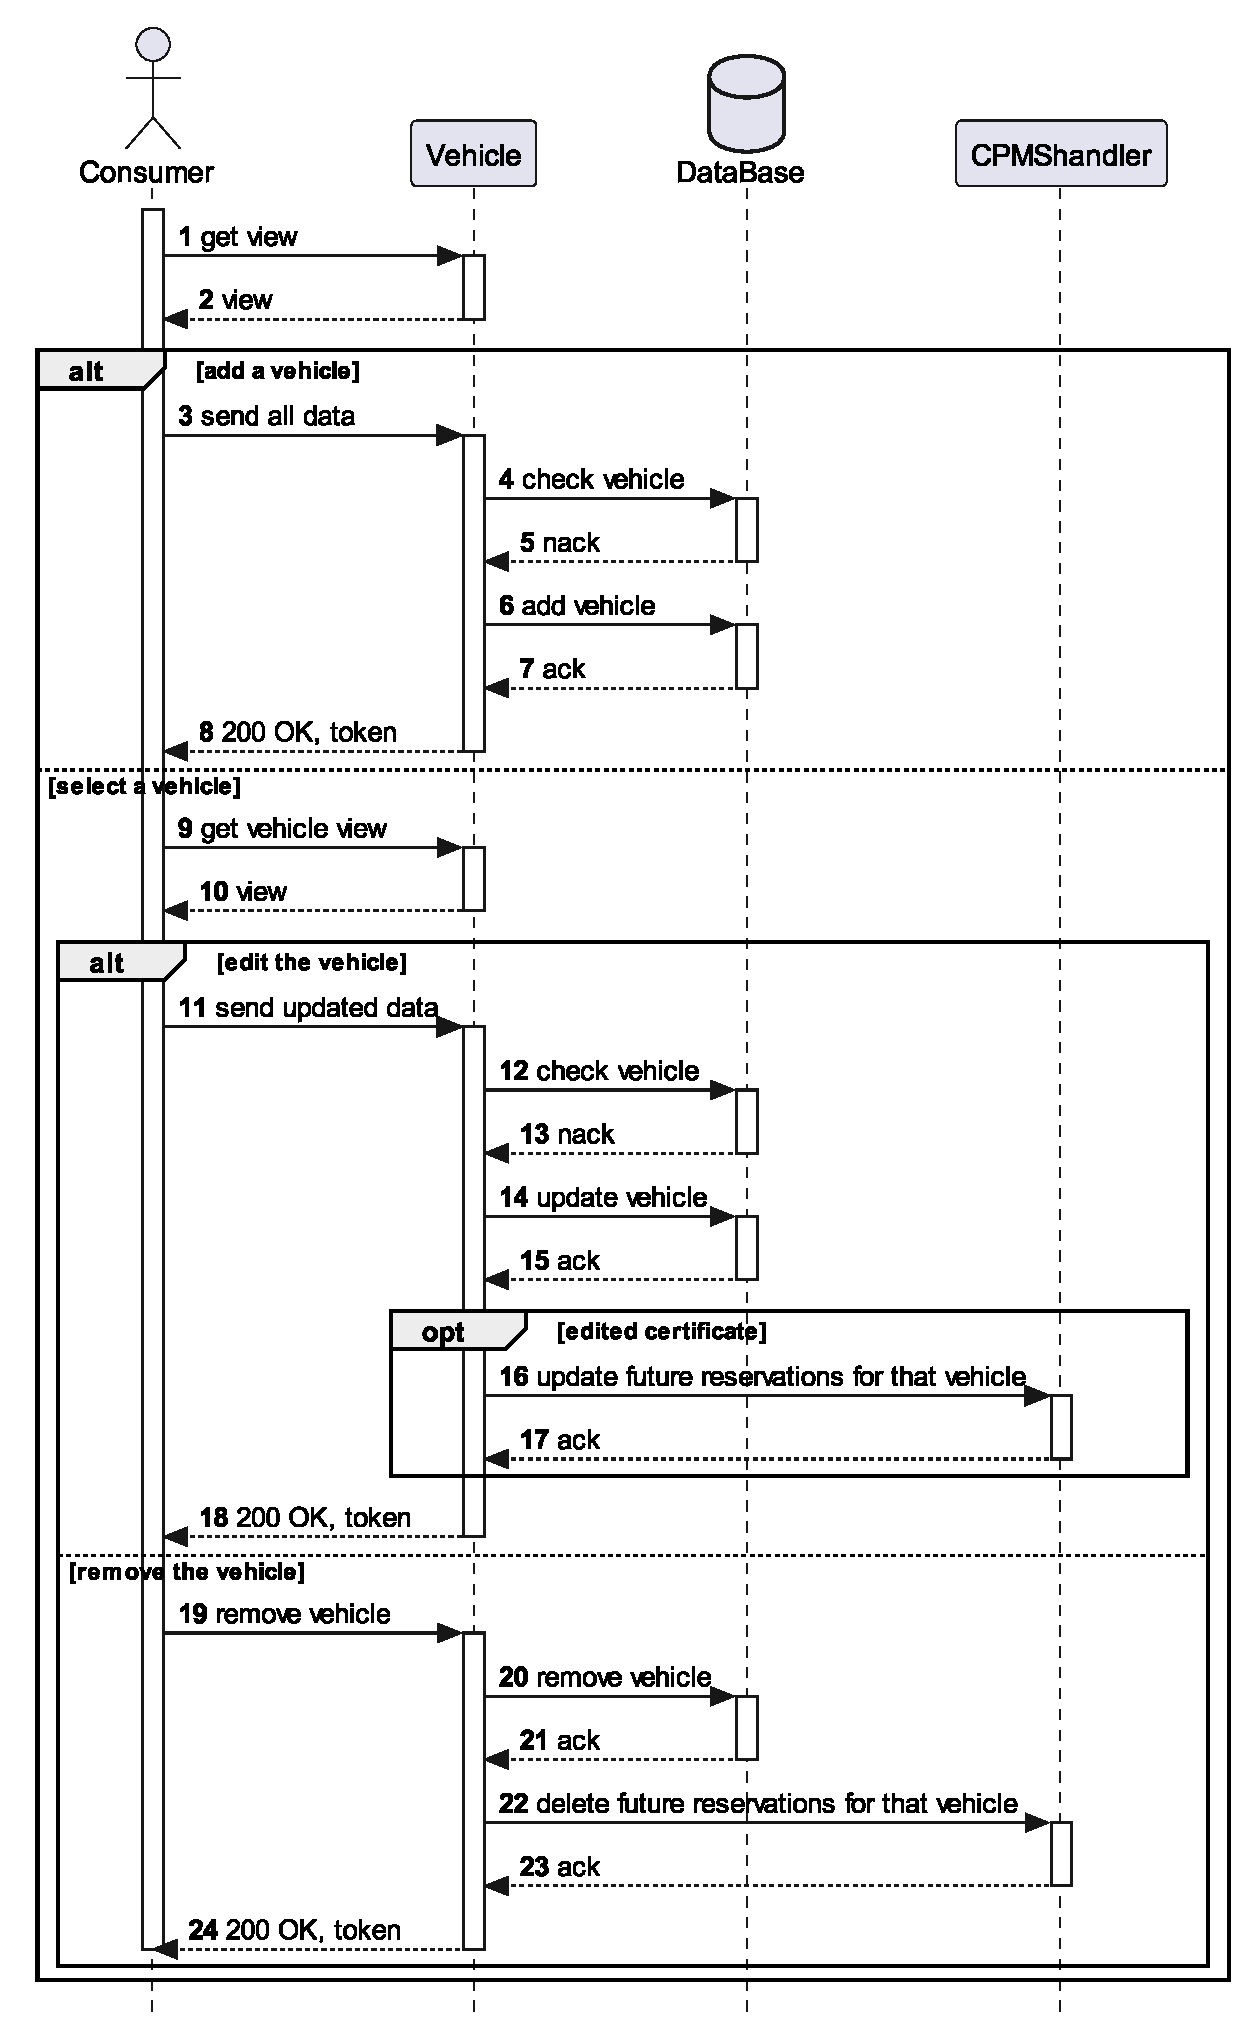
\includegraphics[width=0.71\textwidth]{images/mockups/emsp/vehicles/vehicles}}
        \caption{the page with all the vehicles.}
    \end{minipage}
    \hfill
    \begin{minipage}{0.49\textwidth}
        \centering
        \fbox{\includegraphics[width=0.71\textwidth]{images/mockups/emsp/vehicles/add}}
        \caption{the popup for adding a new vehicle.}
    \end{minipage}
\end{figure}
\begin{figure}[h!]
    \begin{minipage}{0.49\textwidth}
        \centering
        \fbox{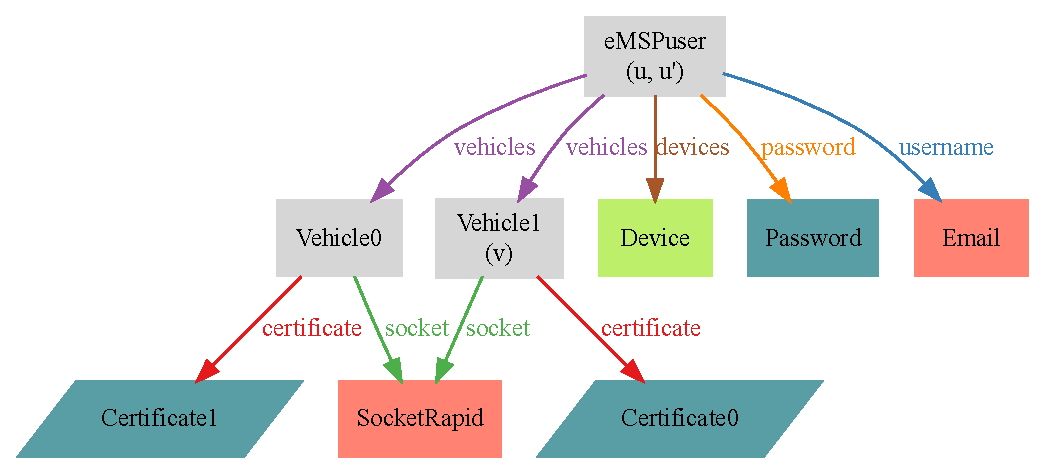
\includegraphics[width=0.71\textwidth]{images/mockups/emsp/vehicles/vehicle}}
        \caption{the details of a vehicle.}
    \end{minipage}
    \hfill
    \begin{minipage}{0.49\textwidth}
        \centering
        \fbox{\includegraphics[width=0.71\textwidth]{images/mockups/emsp/vehicles/edit}}
        \caption{the popup for editing a vehicle.}
    \end{minipage}
\end{figure}

\pagebreak

\paragraph{Payment} Before the user pays from the application the charges, the system shows this page allowing him/her to choose the method s/he prefers for paying. The system supports multiple transaction managers like the ones shown in this interface, but it can be expanded in the future to support more.

\begin{figure}[h!]
    \centering
    \fbox{
\includegraphics[width=0.49\textwidth]{images/mockups/emsp/payment}}
    \caption{the choice of the payment method.}
\end{figure}

\pagebreak

\subsection{Pages connections}

This diagram shows how all the presented interfaces are connected. The white circle at the top left of the diagram presents the starting point, which can be either the opening of the application or the opening of the private area on the eMSP's website.

\begin{figure}[h!]
    \centering
    \includegraphics[width=\columnwidth]{./images/connections/emsp}
    \caption{the connections between the various interfaces.}
\end{figure}

\section{CPMS}

Interactions with the CPMS system are conducted by authorized CPMS users. These users are expected to interact with the CPMS to carry out occasional tasks, as the main system is thought to be automatized. Nonetheless, the CPMS system offers a website capable of allowing all reasonable actions to the users, with an immediate and fairly easy-to-use interface. In this section, mockups of the website are presented to resemble what the actual site could look like. 

\subsection{Interfaces design}

To represent the website for the CPMS system, instances of a \textit{Firefox} browser from a \textit{macOS}-looking operating system are shown, but any browser on any operating system would work, as long as it's running on a working computer. Viewing the website from a mobile phone would be strongly discouraged. 

\paragraph{Login} In order to access the website, users must first login through the login page. The standard username and password are the only requirements, but the system can be expanded to include the need for a second factor for authentication.

\bigskip
\bigskip
\bigskip
\bigskip

\begin{figure}[h!]
    \centering
    \includegraphics[width=\columnwidth]{./images/mockups/cpms/login}
    \caption{CPMS login page.}
\end{figure}

\pagebreak

\paragraph{Home} After login, the web server sends the user the home page, then sends JSON files containing data on DSOs and stations managed by the user. The home page comprehends a brief statistic tab on a selected station for a selected metric, the central tab needed to access the station page of a selected station, and a brief statistic tab on all DSOs available to any of the stations. A button to go to the special offer page sits underneath the station tab. In the top left corner, a menu tab can be clicked to navigate the site, mainly to return to the home page or to go to the offers page. In the top right corner, the user tab can be clicked to see the user information, to change the password, or to log out of the website. In the bottom left corner, buttons are present to help navigate the website, for general information, and to send emails or to call for support. All the tabs and buttons in the corners are also present on the other pages of the website. 

\bigskip
\bigskip
\bigskip
\bigskip

\begin{figure}[h!]
    \centering
    \includegraphics[width=\columnwidth]{./images/mockups/cpms/home}
    \caption{CPMS home page.}
\end{figure}

\pagebreak

\paragraph{Station} By searching (and then clicking on) a charging station, the web server sends the station page, then send data on the sources and DSO available, along with data on the state of the charging columns. On the station page, there are three main tabs. These are periodically updated with new data by the web server. \medskip

The tab in the middle informs the user of the various charging columns present in the charging station, along with information on their socket types and if they are free or occupied at the time of viewing.

\medskip
The left tab is the DSO tab: if the automatic choice is selected (by pressing the button on top), this tab only informs of the DSO available to the station and the prices they offer, along with the currently selected DSO. Otherwise, the user is able to manually and statically select the preferred DSO by clicking on the button on the side of it.
\medskip

The right tab is dedicated to the energy mix. By clicking on the bottom on top the user activates or deactivated the automatic mix choice. If the mix choice is set to manual, users can select if a source can be used or not, and if batteries are present, if these are to be charged or not (batteries cannot be charged while they are in use). The system will still check if illegal states are being reached by the manual choice of an energy mix, and take countermeasures consequently. For example, if not enough power can be obtained by the current setup, and the DSO energy is not being used, the system will automatically set the DSO energy to be used, and will communicate this choice to the user with the next periodic update of the page. Information on the charge level of the batteries and the power obtained from each source is also displayed in this tab.

\bigskip
\bigskip
\bigskip
\bigskip

\begin{figure}[h!]
    \centering
    \includegraphics[width=\columnwidth]{./images/mockups/cpms/Station}
    \caption{Charging station page.}
\end{figure}

\pagebreak

\paragraph{Special offer} In the special offer page, users can see all special offers present, and decide if they want to delete them or create a new special offer. A new special offer is created by clicking on the blue button with the plus sign. A pop-up appears where information on the new special offer is asked: the user has to select a start date (from the current day forward), an end date (that comes after the start date), one charging station affected (or all stations if that's the case) and the percentage amount of the discount. By clicking on \doublequotes{Create} the new special offer is created, by clicking on the \doublequotes{x} mark the whole creation is aborted.

\bigskip
\bigskip
\bigskip
\bigskip

\begin{figure}[h!]
    \centering
    \includegraphics[width=\columnwidth]{./images/mockups/cpms/Offer}
    \caption{Charging station page.}
\end{figure}

\pagebreak

\subsection{Pages connections}

This diagram shows how all the presented interfaces are connected. The white circle at the top left of the diagram presents the user opening the web page.

\begin{figure}[h!]
    \centering
    \includegraphics[width=\columnwidth]{./images/connections/cpms}
    \caption{the connections between the various interfaces.}
\end{figure}

    \chapter{Requirements Traceability} \label{traceability}

It's important to check that all the requirements pointed out into the \textit{Requirements Analysis and Specification Document} of the \textsc{eMall} project are actually satisfied into the design of the system. That's why in this section every requirement is mapped into one or more components of the system.

\section{Requirements}

For reference purposes, here are reported all the requirements for the systems, divided into \textit{eMSP requirements} and \textit{CPMS requirements}.

\subsection{eMSP requirements}

\begin{center}
    \begin{tabular}{ | >{\centering\arraybackslash}m{0.1\columnwidth} | >{\arraybackslash}m{0.84\columnwidth} | }
        \hline
        \textbf{Identifier} & \multicolumn{1}{c|}{\textbf{Description}} \\
        \hline
        \hline
        \showR{r:e:signup} & The system must allow the user to sign-up. \\
        \hline
        \showR{r:e:signup_check} & The system must check the sign-up data. \\
        \hline
        \showR{r:e:signup_mail} & The system must send the user an email for activating the account after a successful sign-up. \\
        \hline
        \showR{r:e:signup_activation} & The system must discard any account activation request that arrives after 24 hours from the sign-up procedure. \\
        \hline
        \showR{r:e:signup_not_activated} & The system must consider any signed-up user who hasn't already activated the account as an unregistered user. \\
        \hline
        \showR{r:e:signup_success} & The system must notify the user of the sign-up result, sending an email if it's successful. \\
        \hline
        \showR{r:e:login} & The system must allow the user to log in. \\
        \hline
        \showR{r:e:login_check} & The system must check the login data. \\
        \hline
        \showR{r:e:pwchange} & The system must allow the user to change his/her password after logging in. \\
        \hline
        \showR{r:e:pwreset} & The system must allow any registered user to reset his/her password by sending an email to the specified address. \\
        \hline
        \showR{r:e:pwreset_timeout} & The system must discard any password change 24 hours after the request. \\
        \hline
        \showR{r:e:pwreset_duplicate} & The system must discard any duplicated usage of the same link for password change after a successful one. \\
        \hline
        \showR{r:e:logout} & The system must allow the user to logout. \\
        \hline
        \showR{r:e:notification} & The system must allow the user to set the preferred notification method. \\
        \hline
        \showR{r:e:car_add} & The system must allow the user to add a new vehicle. \\
        \hline
        \showR{r:e:car_remove} & The system must allow the user to remove an associated vehicle, only if there is at least one. \\
        \hline
        \showR{r:e:car_edit} & The system must allow the user to edit any associated vehicle's details. \\
        \hline
        \showR{r:e:stations_lookup} & The system must allow the user to look for nearby stations. \\
        \hline
        \showR{r:e:stations_sort} & The system must allow the user to sort the nearby stations according to distance, price, and availability. \\
        \hline
        \showR{r:e:stations_favorite_mark} & The system must allow the user to mark and unmark stations as \doublequotes{favorite}. \\
        \hline
        \showR{r:e:book} & The system must allow the user to book a charge in a charging station if any slot is available. \\
        \hline
        \showR{r:e:book_car} & The system must ask the user the vehicle s/he wants to charge every time s/he books a charge. \\
        \hline
    \end{tabular}
\end{center}
\begin{center}
    \begin{tabular}{ | >{\centering\arraybackslash}m{0.1\columnwidth} | >{\arraybackslash}m{0.84\columnwidth} | }
        \hline
        \textbf{Identifier} & \multicolumn{1}{c|}{\textbf{Description}} \\
        \hline
        \hline
        \showR{r:e:book_notification} & The system must notify the user of any successful booked charge. \\
        \hline
        \showR{r:e:book_add_calendar} & The system must allow the user to add any booked charge to the calendar. \\
        \hline
        \showR{r:e:book_all} & The system must allow the user to show all the booked charges, both past, and future (there might be limits). \\
        \hline
        \showR{r:e:book_edit} & The system must allow the user to edit or delete a booked charge before the end of the booked slot. \\
        \hline
        \showR{r:e:book_notification_slot} & The system must notify the user of the charging slot to use before the charge. \\
        \hline
        \showR{r:e:book_notification_end} & The system must notify the user when the charge is finished. \\
        \hline
        \showR{r:e:payment} & The system must allow the user to pay for the obtained service. \\
        \hline
        \showR{r:e:payment_notification} & The system must notify the user after every payment attempt (both in case of success and failure). \\
        \hline
        \showR{r:e:eroaming} & The system must periodically contact an eRoaming service for obtaining the list of available CPOs (and respective CPMSs). \\
        \hline
        \showR{r:e:cpms_connect} & The system must be able to connect to any CPMS that offers standard APIs. \\
        \hline
        \showR{r:e:cpms_communicate} & The system must be able to communicate with any connected CPMS through standard APIs. \\
        \hline
        \showR{r:e:user_registered} & The system must allow any registered user to do everything specified, except signing up. \\
        \hline
        \showR{r:e:user_unregistered} & The system must allow any unregistered user to only sign up and log in. \\
        \hline
        \showR{r:e:notification_app} & The system must send the notification only to the user's authenticated devices if the notification preference is by in-app notification. \\
        \hline
        \showR{r:e:notification_mail} & The system must send emails instead of in-app notifications if that's the user's preferred method or if there is no available user's device. \\
        \hline
    \end{tabular}
\end{center}

\subsection{CPMS requirements}

\begin{center}
    \begin{tabular}{ | >{\centering\arraybackslash}m{0.1\columnwidth} | >{\arraybackslash}m{0.84\columnwidth} | }
        \hline
        \textbf{Identifier} & \multicolumn{1}{c|}{\textbf{Description}} \\
        \hline
        \hline
        \showR{r:c:input} & The system must check all input data correctness. \\
        \hline
        \showR{r:c:login} & The system must allow the user to log in. \\
        \hline
        \showR{r:c:pwchange} & The system must allow the user to change his/her password after logging in. \\
        \hline
        \showR{r:c:pwreset} & The system must allow any registered user to reset his/her password by sending an email to the specified address. \\
        \hline
        \showR{r:c:pwreset_timeout} & The system must discard any password change 24 hours after the request. \\
        \hline
        \showR{r:c:pwreset_duplicate} & The system must discard any duplicated usage of the same link for password change after a successful one. \\
        \hline
        \showR{r:c:logout} & The system must allow the user to logout. \\
        \hline
        \showR{r:c:API_show_booking} & The system must provide an API function to get information about all bookings present for any charging station. \\
        \hline
        \showR{r:c:API_book} & The system must provide an API function to add/delete a booking for a charging point in a charging station. \\
        \hline
        \showR{r:c:API_stations} & The system must provide an API function to get information about all charging points and respective sockets in a charging station. \\
        \hline
        \showR{r:c:API_prices} & The system must provide an API function to get information about prices relative to a charging station and socket types. \\
        \hline
        \showR{r:c:start_car_charge} & The system must start charging a car when it is first plugged in if it corresponds to the car for which a charge was booked in the corresponding time and place (same charging point/socket as well). \\
        \hline
        \showR{r:c:stop_car_charge_full} & The system must stop charging a car once it recognizes that the car battery has reached full capacity. \\
        \hline
        \showR{r:c:stop_car_charge_time} & The system must stop charging a car if the booking corresponding to that car ends and the car is still plugged in. \\
        \hline
        \showR{r:c:autoselect_DSO} & The system must automatically select the DSO that offers the best energy price if the “automatic DSO choice” is selected. \\
        \hline
    \end{tabular}
\end{center}
\begin{center}
    \begin{tabular}{ | >{\centering\arraybackslash}m{0.1\columnwidth} | >{\arraybackslash}m{0.84\columnwidth} | }
        \hline
        \textbf{Identifier} & \multicolumn{1}{c|}{\textbf{Description}} \\
        \hline
        \hline
        \showR{r:c:stop_battery_charge_full} & If a battery was charging and reaches a full charge, the system must stop charging the battery. \\
        \hline
        \showR{r:c:auto_mix} & The system must automatically change the energy mix if the \doublequotes{automatic mix choice} is selected. \\
        \hline
        \showR{r:c:notification_column} & The system must automatically notify the eMSP of the assignment of a charging column. \\
        \hline
        \showR{r:c:notification_charge} & The system must automatically notify the eMSP of the end of the car charge. \\
        \hline
        \showR{r:c:periodical_updates} & The system must periodically update the database with new data coming from sensors present in charging stations. \\
        \hline
        \showR{r:c:view_bookings} & The system must allow the CPMS user to view all bookings present for any charging station. \\
        \hline
        \showR{r:c:view_charging_point} & The system must allow the CPMS user to view all charging points, relative socket types, and if they are occupied or not, for any charging station. \\
        \hline
        \showR{r:c:view_battery_levels} & The system must allow the CPMS user to view the batteries' charge levels if present. \\
        \hline
        \showR{r:c:manage_offers} & The system must allow the CPMS user to create and delete special charge offers. \\
        \hline
        \showR{r:c:view_DSO} & The system must allow the CPMS user to view all DSO available. \\
        \hline
        \showR{r:c:view_DSO_prices} & The system must allow the CPMS user to view all DSO prices. \\
        \hline
        \showR{r:c:change_mix} & The system must allow the CPMS user to change the energy mix. \\
        \hline
        \showR{r:c:start_battery_charge} & The system must allow the CPMS user to start recharging batteries if they are present. \\
        \hline
        \showR{r:c:auto_DSO} & The system must allow the CPMS user to activate and deactivate \doublequotes{automatic DSO choice}. \\
        \hline
        \showR{r:c:auto_MIX} & The system must allow the CPMS user to activate and deactivate \doublequotes{automatic mix choice}. \\
        \hline
        \showR{r:c:DSO_payment} & The system must allow the CPMS user to modify the automatic DSO payment method. \\
    \hline
    \end{tabular}
\end{center}

\section{Mapping with components}

\begin{center}
    \begin{tabular}{ | >{\centering\arraybackslash\bfseries}m{0.06\columnwidth} | >{\arraybackslash}m{0.15\columnwidth} | >{\arraybackslash}m{0.34\columnwidth} | >{\arraybackslash}m{0.34\columnwidth} | }
        \hline
        Goal & \multicolumn{1}{c|}{\textbf{Requirements}} & \multicolumn{1}{c|}{\textbf{eMSP components}} & \multicolumn{1}{c|}{\textbf{CPMS components}} \\
        \hline
        \hline
        \refG{g:e:lookup} & \refR{r:e:signup}-\refR{r:e:notification}, \refR{r:e:stations_lookup}-\refR{r:e:stations_favorite_mark}, \refR{r:e:eroaming}-\refR{r:e:user_unregistered} & \texttt{CPMShandler}, \texttt{DatabaseHandler}, \texttt{eRoamingHandler}, \texttt{User}, \texttt{Web server} & \texttt{APIhandler}, \texttt{DatabaseHandler}, \texttt{eRoamingHandler} \\
        \hline
        \refG{g:e:book} & \refR{r:e:signup}-\refR{r:e:car_edit}, \refR{r:e:book}-\refR{r:e:book_notification_slot}, \refR{r:e:cpms_communicate}-\refR{r:e:notification_mail} & \texttt{BookingHandler}, \texttt{CPMShandler}, \texttt{DatabaseHandler}, \texttt{Device}, \texttt{EmailHandler}, \texttt{User}, \texttt{Vehicle}, \texttt{Web server} & \texttt{APIhandler}, \texttt{Booking}, \texttt{DatabaseHandler} \\
        \hline
        \refG{g:e:start} & \refR{r:e:car_add}-\refR{r:e:car_edit}, \refR{r:e:cpms_communicate}-\refR{r:e:user_unregistered} & \texttt{DatabaseHandler}, \texttt{User}, \texttt{Vehicle}, \texttt{Web server} & \texttt{DatabaseHandler}, \texttt{ChargingColumn}, \texttt{ChargingStation} \\
        \hline
        \refG{g:e:notify} & \refR{r:e:signup}-\refR{r:e:car_edit}, \refR{r:e:book_notification_end}, \refR{r:e:cpms_communicate}-\refR{r:e:notification_mail}, \refR{r:c:notification_column}, \refR{r:c:notification_charge} & \texttt{APIhandler}, \texttt{DatabaseHandler}, \texttt{Device}, \texttt{EmailHandler}, \texttt{User} &\texttt{DatabaseHandler}, \texttt{ChargingStation}, \texttt{eMSPhandler} \\
        \hline
        \refG{g:e:pay} & \refR{r:e:signup}-\refR{r:e:car_edit}, \refR{r:e:payment}, \refR{r:e:payment_notification}, \refR{r:e:user_registered}-\refR{r:e:notification_mail} & \texttt{CPMShandler}, \texttt{DatabaseHandler}, \texttt{Device}, \texttt{EmailHandler}, \texttt{PaymentHandler}, \texttt{User}, \texttt{Web server} & \texttt{APIhandler}, \texttt{ChargingColumn}, \texttt{DatabaseHandler}, \texttt{eMSPhandler}, \texttt{PaymentHandler} \\
        \hline
        \refG{g:c:info} & \refR{r:e:book}, \refR{r:e:book_all}-\refR{r:e:book_notification_slot}, \refR{r:c:API_show_booking}-\refR{r:c:API_prices}, \refR{r:c:periodical_updates}-\refR{r:c:view_battery_levels} & \texttt{CPMShandler} & \texttt{APIhandler}, \texttt{ChargingColumn}, \texttt{ChargingStation}, \texttt{DatabaseHandler} \\
        \hline
        \refG{g:c:charge} & \refR{r:c:API_show_booking}, \refR{r:c:start_car_charge}-\refR{r:c:stop_car_charge_time}, \refR{r:c:notification_column}, \refR{r:c:notification_charge} & None & \texttt{ChargingColumn}, \texttt{ChargingStation}, \texttt{DatabaseHandler} \\
        \hline
        \refG{g:c:dso} & \refR{r:c:input}-\refR{r:c:logout}, \refR{r:c:autoselect_DSO}, \refR{r:c:view_DSO}, \refR{r:c:view_DSO_prices}, \refR{r:c:auto_DSO}, \refR{r:c:DSO_payment} & None & \texttt{ChargingStation}, \texttt{DatabaseHandler}, \texttt{DSOhandler}, \texttt{User}, \texttt{Web server} \\
        \hline
        \refG{g:c:mix} & \refR{r:c:input}-\refR{r:c:logout}, \refR{r:c:stop_battery_charge_full}, \refR{r:c:auto_mix}, \refR{r:c:change_mix}, \refR{r:c:start_battery_charge}, \refR{r:c:auto_MIX} & None & \texttt{ChargingStation}, \texttt{DatabaseHandler}, \texttt{EnergySource}, \texttt{User}, \texttt{Web server} \\
        \hline
        \refG{g:c:offers} & \refR{r:c:input}-\refR{r:c:logout}, \refR{r:c:API_prices}, \refR{r:c:manage_offers}, \refR{r:c:view_DSO_prices} & None & \texttt{DatabaseHandler}, \texttt{SpecialOffer}, \texttt{User}, \texttt{Web server} \\
        \hline
    \end{tabular}
\end{center}

    \chapter{Implementation, Integration and Test Plan} \label{iitp}

\section{Introduction}

After having described all the components of the system and their interconnections, this chapter describes how these should be implemented, integrated, and tested in order to have two fully working systems: the eMSP's and the CPMS's.\medskip

In general, the method followed for building up both of the systems is to first start with a bottom-up approach to create the component that directly interacts with the database, to have a fully working data retrieval and management. Then a thread approach is used to develop all the other components in parallel (maybe even across multiple teams), dividing the work by functionality. Meanwhile, it's possible to test the correct functioning of every part of the system and to provide some betas of the software to the stakeholders\footnote{The \textit{stakeholders} are the ones who own shares in an enterprise.}, to let them check that all the required functionalities have been implemented according to their needs and desires.

\subsection{Terminology}

\paragraph{Development strategies} Just to be even more clear, here we provide a brief description of some strategies nominated in this section. There are references to the components interfaces of the two systems that can be found in \reference{view:interfaces}.
\begin{itemize}
    \item \textit{Bottom-up approach}: the bottom-up approach consists in starting building the system from its foundations, which is made of the components in the leaves of a \doublequotes{uses} hierarchy. Starting from there, the strategy goes up to the root of the hierarchy.
    \item \textit{Thread approach}: the thread approach focuses more on developing specific functionalities across multiple components, thus developing a single piece of all the touched components.
\end{itemize}

\paragraph{Testing strategies} Testing software is not trivial and there are multiple methods for doing it. Every strategy has its own goals and here are reported the ones nominated in this chapter.
\begin{itemize}
    \item \textit{Load testing}: this kind of test helps to identify eventual memory leaks, buffer overflows, and in general any problem related to memory usage. Even though the choice of the language (or languages) to use is not enforced here, we suggest using the Rust language for avoiding these kinds of errors.
    \item \textit{Performance testing}: its main purpose is to identify any bottleneck of the application, therefore affecting response times and general throughput.
    \item \textit{Stress testing}: the main purpose of a stress test is to check if the system is able to gracefully adapt and recover after some failures.
    \item \textit{Unit testing}: this testing is done in order to check whether the functions of the system (or groups of them) do what they are supposed to.
\end{itemize}

\vfill

\pagebreak

\section{eMSP}

First, here we provide the description of how the eMSP should be implemented, integrated, and tested. The flow follows the general description provided above in the introduction.

\subsection{Implementation plan}

\paragraph{Step 1 (bottom-up)}\label{emsp:bottomup} As stated in the introduction, the implementation should start with a bottom-up approach, by first implementing the \texttt{DatabaseHandler}, which is the component in charge of providing all the data to the above layers of the business layer and to do some processing with them. During this phase, it's also suggested to start developing the internal functions of the \texttt{PaymentHandler} and the \texttt{EmailHandler} (in this last case, like the methods for connecting to the SMTP server and general methods for building up and sending the emails).

\paragraph{Step 2 (thread)}\label{emsp:thread} After having fully developed the \texttt{DatabaseHandler}, the rest of the components should be developed in parallel following a thread approach, first focusing on the main functionalities that the eMSP should provide, and then moving to the other ones (like the password reset, the account activation procedure\dots). Together with this, the NGINX configuration should be created and updated in order to allow it to redirect the traffic accordingly to the various components.

\paragraph{Step 3 (frontend)}\label{emsp:frontend} While developing all the components presented in the previous step, the frontend can also be developed, possibly following the development of the various functionalities, but it's not mandatory. In case of problems, it's possible to easily change the frontend JavaScript querying and displaying functions.

\subsection{Integration plan}

The integration plan roughly follows the implementation plan presented above.

\paragraph{Components of \nameref{emsp:bottomup}} These few components should be integrated with the other ones following the developed threads.

\paragraph{Components of \nameref{emsp:thread}} Since the main part of the development is done following a thread-based approach, the integration of many of the components is done directly while developing them. Integrating the various threads, instead, should be done whenever any thread is completed.

\paragraph{Components of \nameref{emsp:frontend}} The frontend should be integrated with the underlying components as soon as the functionalities have been developed, in order to also provide some betas of the software to the stakeholders.

\subsection{Test plan}

The test plan for the system is slightly more complex than what was done in with the previous plans.\medskip

For every component or thread, after it has been developed, a unit test should be performed in order to immediately spot any possible bug in the implementation.\medskip

Moreover, for any completed thread, some other tests should be performed in order to discover some other more subtle bugs in the software and to possibly optimize the performance of the whole system:
\begin{itemize}
    \item \textit{Performance testing}: this is done for spotting the bottlenecks.
    \item \textit{Load testing}: this is done to identify memory leaks, overflows or other memory-related problems.
    \item \textit{Stress testing}: its purpose is instead to recover gracefully after failures.
\end{itemize}

Once any beta version of the software is available, it's possible to perform some acceptance testing which should be conducted by different people, maybe also the stakeholders, for testing the usability of the system.

\pagebreak

\section{CPMS}

We'll now describe how the CPMS system should be implemented, integrated, and tested. The flow follows the general description provided above in the introduction.

\subsection{Implementation plan}

\paragraph{Step 1 (bottom-up)}\label{cpms:bottomup} As stated in the introduction, the implementation should start with a bottom-up approach, by first implementing the \texttt{DatabaseHandler}, which is the component in charge of providing all the data to the above layers of the business layer and to do some processing with them. After the \texttt{DatabaseHandler} is completed, The \texttt{ChargingStation}, \texttt{ChargingColumn}, and \texttt{EnergySource} should be implemented, and possibly be connected to their physical counterparts or to similar components. 

\paragraph{Step 2 (thread)}\label{cpms:thread} After having fully developed the components mentioned in step one, the rest of the components should be developed in parallel following a thread approach, first focusing on the main functionalities that the CPMS should provide, like the booking mechanism. After those, the focus should be on the components that interact with, or offer, external interfaces. Together with this, the NGINX configuration should be created and updated in order to allow it to redirect the traffic accordingly to the various components.

\paragraph{Step 3 (frontend)}\label{cpms:frontend} While developing all the components presented in the previous steps, the frontend can also be developed, possibly following the development of the various functionalities, but it's not mandatory. In case of problems, it's possible to easily change the frontend JavaScript querying and displaying functions.

\subsection{Integration plan}

The integration plan roughly follows the eMSP implementation plan.

\paragraph{Components of \nameref{cpms:bottomup}} The components implemented in the bottom-up approach should all be integrated as they are developed, making use of mockup physical counterparts to ensure their correct functioning.

\paragraph{Components of \nameref{cpms:thread}} Since the main part of the development is done following a thread-based approach, the integration of many of the components is done directly while developing them. Integrating the various threads, instead, should be done whenever any thread is completed.

\paragraph{Components of \nameref{cpms:frontend}} The frontend should be integrated with the underlying components as soon as the functionalities have been developed, in order to also provide some betas of the software to the stakeholders.

\subsection{Test plan}

The test plan for the CPMS system should roughly follow the same test plan for the eMSP system. \medskip

For every component or thread, after it has been developed, a unit test should be performed in order to immediately spot any possible bug in the implementation.\medskip

Tests for the \texttt{ChargingColumn}, the \texttt{ChargingStation}, and the \texttt{EnergySource} should be conducted on their physical counterparts as well as on the components.

Moreover, for any completed thread, the same tests specified for the eMSP system should be performed in order to discover some other more subtle bugs in the software and to possibly optimize the performance of the whole system:
\begin{itemize}
    \item \textit{Performance testing}: this is done for spotting the bottlenecks.
    \item \textit{Load testing}: this is done to identify memory leaks, overflows, or other memory-related problems.
    \item \textit{Stress testing}: its purpose is instead to recover gracefully after failures.
\end{itemize}

Once any beta version of the software is available, it's possible to perform some acceptance testing which should be conducted by different people, maybe also the stakeholders, for testing the usability of the system.

Particular attention should be paid to how the physical elements behave when the system is in place, and tests should be done while consulting specialists in the electronic components to ensure the success of the system.
    \chapter{Conclusions} \label{conclusions}

\section{Final thoughts}

This document was redacted following the guidelines for the project (\textit{eMall - e-Mobility for All project}). Discrepancies between our document and the guidelines are to be considered our hypothesis on how the two systems should behave or be modeled.\medskip

Also, these systems have been designed having in mind possible future expansions. Thus, anyone who wants to expand this project is welcome and encouraged to do so. For example, one possibility is to set a limit after which the user is no more allowed to book charges until s/he decides to pay the previous ones.

\section{Credits}

For writing this document, we used different pieces of software and materials from the Internet. This is a rather comprehensive list of them:
\begin{itemize}
    \item \href{https://www.latex-project.org/}{\textit{\LaTeX} (with packages)} and \href{https://code.visualstudio.com/}{\textit{Visual Studio Code} (with plugins)} for writing the document.
    \item \href{https://git-scm.com/}{\textit{Git}}, \href{https://github.com/}{\textit{GitHub}} and \href{https://www.notion.so/}{\textit{Notion}} for keeping things organized.
    \item \href{https://www.diagrams.net/}{\textit{draw.io}} and \href{https://plantuml.com/}{\textit{PlantUML}} for creating the diagrams.
    \item \href{https://fonts.google.com/icons}{\textit{Google Fonts} (icon library)}, \href{https://inkscape.org/}{\textit{Inkscape}}, \href{https://www.openstreetmap.org/}{\textit{OpenStreetMap}}, \href{https://penpot.app/}{\textit{Penpot}} (with designs from \href{https://ape.wtf/}{ApeWTF} and \href{https://design.google/library/designing-material/}{Google}) and \href{https://www.wikipedia.org/}{\textit{Wikipedia}} for drawing the mockups.
\end{itemize}

\section{Effort}

\begin{center}
    \begin{tabular}{ | >{\arraybackslash}m{0.52\columnwidth} | >{\centering\arraybackslash}m{0.2\columnwidth} | >{\centering\arraybackslash}m{0.2\columnwidth} | }
        \hline
        \multicolumn{1}{|c|}{\textbf{Task}} & \textbf{Riccardo Motta} & \textbf{Pierluigi Negro} \\
        \hline
        \hline
        Writing chapter 1 & 3h & 2h \\
        \hline
        Writing chapter 2 & 4h & 4h \\
        \hline
        Drawing overview, composition diagrams, component views and deployment view & 6h & 7h \\
        \hline
        Drawing runtime views and components interfaces & 4h & 8h \\
        \hline
        Writing chapter 3 & 2h & 1h \\
        \hline
        Designing the mockups & 20h & 18h \\
        \hline
        Creating the pages connections diagrams & 2h & 1h \\
        \hline
        Mapping components and requirements and writing chapter 4 & 2h & 2h \\
        \hline
        Writing chapter 5 & 3h & 1h \\
        \hline
        Other related work & 5h & 4h \\
        \hline
        Updating document for Version 1.1 & 0.5h & 0.5h \\
        \hline
        \hline
        \textbf{Total} & \textbf{51.5h} & \textbf{48.5h} \\
        \hline
    \end{tabular}
\end{center}


\end{document}
